\documentclass [11pt,a4paper,twoside,english,spanish]{bmpthesis}
\addbibresource{References.bib}

\definecolor{redish}{RGB}{255,10,10}

\Author{Ignacio Ortiz de Zúñiga Mingot}
\Date{July de 2022}
\Degree{Master universitario en ingeniería industrial}
\Keywords{Artificial vision, Sintetic database, YOLO, Pick & Place}
\Subject{Trabajo de Final de Master}
\Supervisors{Álvaro Jesús López López, Ignacio de Rodrigo Tobías}
\Title{Sistema de visión artificial basado en un dataset sintético para una aplicación de Pick and Place}
\Footer{Sistema de visión artificial para una aplicación de Pick and Place}

\begin{document}

% Documentos para formalizar el TFM
\frontmatter
\Frontcover
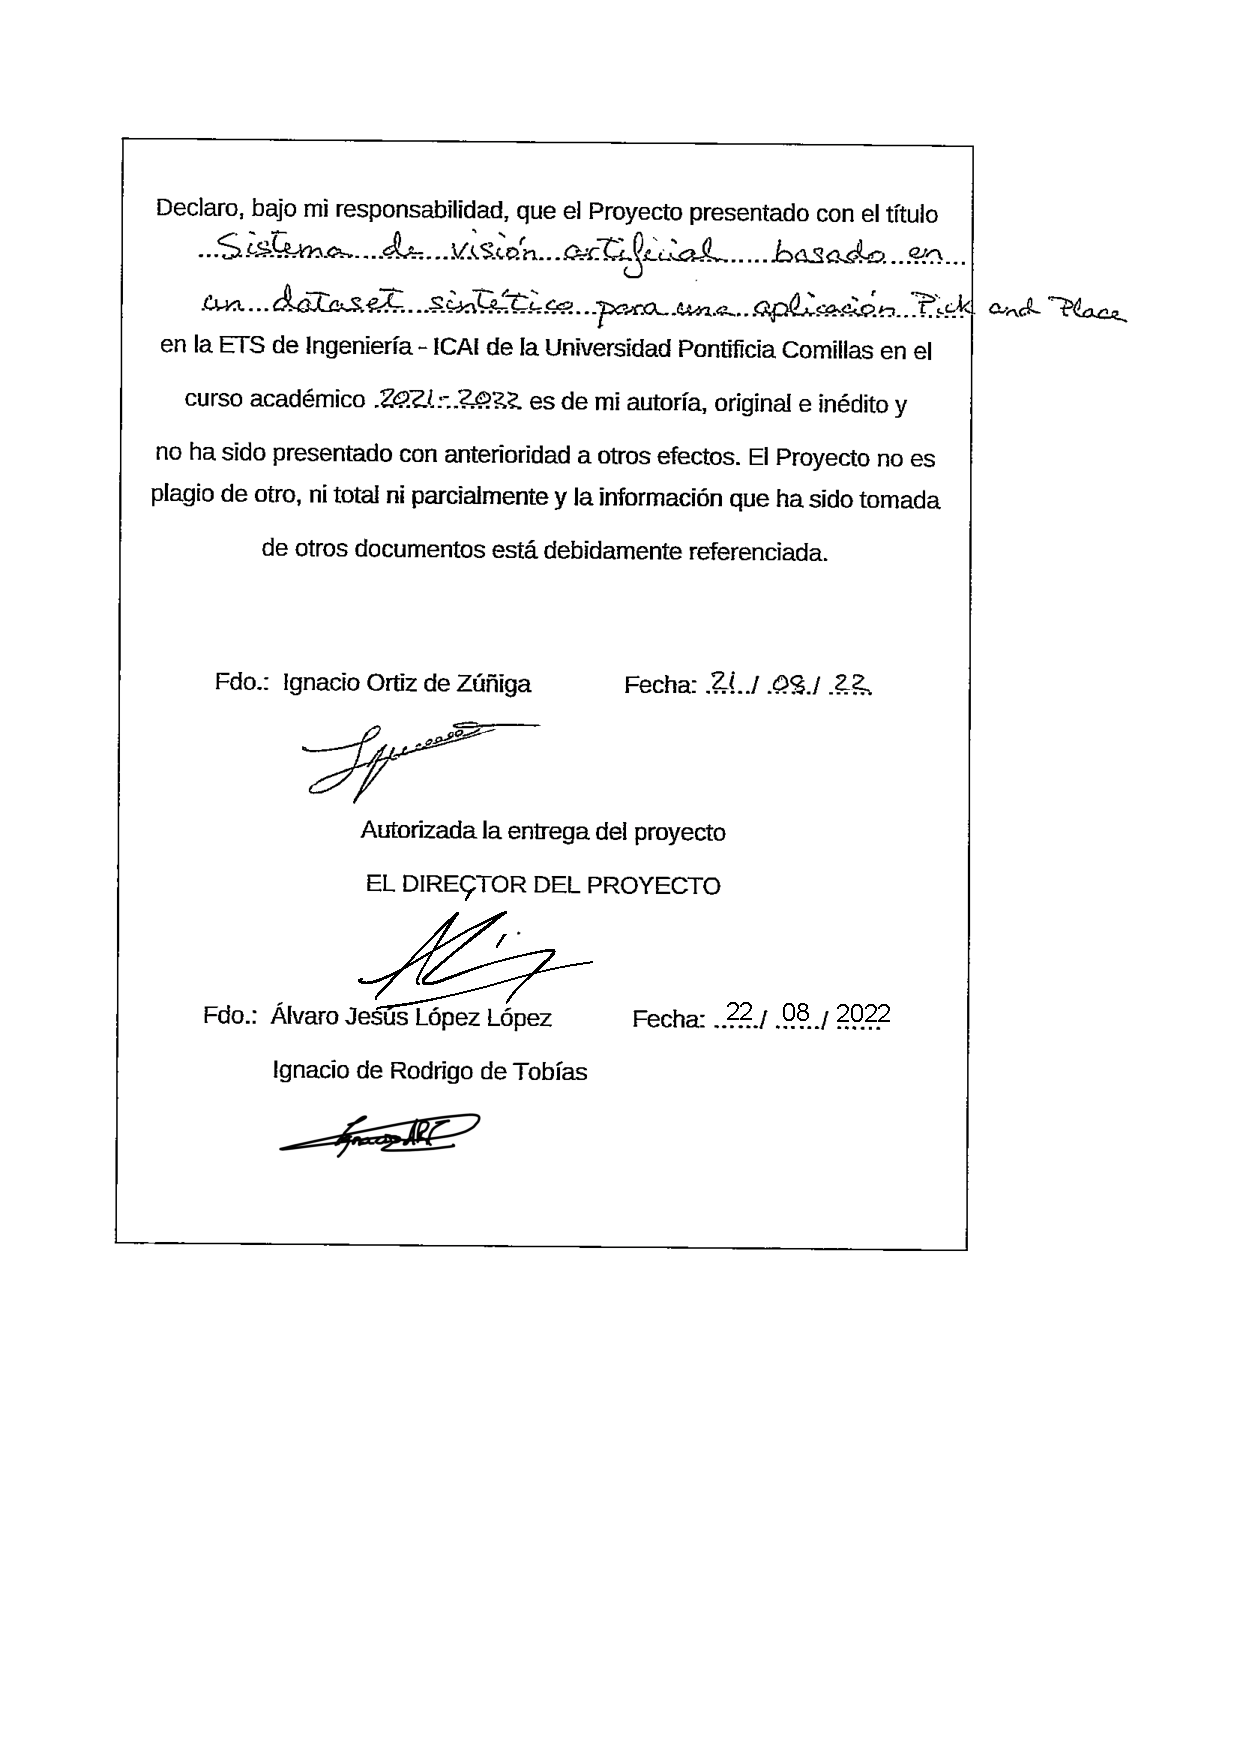
\includepdf{AnexoI.pdf}

\frontmatter
\Frontcover

\Dedication{Para todos los que me habéis soportado \\ durante estos largos años de carrera}
\FrontmatterChapterNoToC{Agradecimientos}
En desarrollo...

\TableOfContents
\ListOfFigures
\ListOfTables
%\ListOfAlgorithms
\Acronyms

% Resumen del proyecto
\FrontmatterChapter{Resumen}
{\setlength{\parindent}{0pt}
\begin{Large}
\textbf{OPTIMIZACIÓN DEL SISTEMA DE VISIÓN ARTIFICIAL DE UN ROBOT INDUSTRIAL PARA UNA APLICACIÓN DE PICK AND PLACE}
\end{Large}

\textbf{Autor: Ortiz de Zúñiga Mingot, Ignacio.} \\
Directores: Boal Martín-Larrauri, Jaime y Rodríguez Mondéjar, José Antonio. \\
Entidad colaboradora: ICAI – Universidad Pontificia Comillas \\

\section*{Resumen del proyecto}
En la última década se ha producido revolución industrial conocida como industria 4.0 gracias a los numerosos avances en el sector de la robótica. Este cambio se ha visto producido gracias a que con el desarrollo de los robots se ha conseguido dotar a estos de capacidades para completar tareas previamente imposibles para el ser humano y con un rendimiento y rapidez superior. Es por ello que se decidió implantar dichos sistemas en un robot industrial de Comillas ICAI con el fin de que este sea capaz de recolectar piezas de LEGO dispuestas de forma aleatoria sobre una mesa de trabajo. En este proyecto se parte de este sistema basado en la segmentación clásica y se mejora y actualiza con el desarrollo de sistemas basados en redes neuronales y aprendizaje profundo. Se han desarrollado múltiples redes de diferentes tamaños basadas en R-CNN, Faster R-CNN y YOLO y se camparan entre si y frente al sistema de segmentación clásico. \\
\textbf{Palabras clave:} Visión artificial, Redes neuronales, AlexNet, VGG-16, R-CNN, Faster R-CNN, YOLO, Robótica, LEGO

\section*{1. Introducción}
Durante los últimos dos años se ha desarrollado un sistema que dote de visión artificial y autonomía a los robots de Comillas ICAI. La tarea escogida para llevar a cabo con estos robots es la recolección de piezas de LEGO dispuesta de forma aleatoria en una zona de trabajo. Este proyecto surge como la evolución de estos sistemas con el fin de mejorar el subsistema de visión artificial mejorando así las capacidades del robot. Para ello primero se ha mejorado el sistema presente con el desarrollo de nuevos análisis más detallados y precisos. Este sistema se basa en el filtrado con máscaras de color, la detección de bordes y la transformada de Hough. Además, se han desarrollado nuevos sistemas para el cálculo de la profundidad y el cálculo de la orientación de la pieza. Sin embargo, a pesar de estas mejoras se ha observado que este sistema no puede competir con los sistemas más modernos ya implantados en la industria. Es por ello que se han desarrollado nuevos sistemas basados en redes neuronales convolucionales. Tal y como su nombre indica estos se basan en el principio de la convolución y el aprendizaje profundo. Con la ayuda de una base de datos son capaces de extraer las características de un objeto y aprender a identificarlo. Es por ello que se a optado por dotar de esta tecnología a los sistemas previos para mejorarlos y así perfeccionar los.

\section*{2. Metodología}
El sistema de visión artificial implantado en el brazo robótico esta constituido por tres elementos que deben de cooperar entre si y comunicarse a través de conexiones USB y TCP/IP. La captura de imágenes se realiza con una cámara Intel Realsense D435 que cuenta con sensores RGB y de profundidad y ha sido conectada a través de una conexión USB. El procesado de las imágenes RGB y de profundidad es llevado a cabo por un ordenador con la ayuda de MATLAB. Y por último,se mandarán las instrucciones conteniendo la posición, altura y orientación de cada pieza a través de una conexión TCP/IP al brazo robótico IRB 120. Esta estructura se puede ver en la \autoref{fig:resm1}

%\begin{figure}[ht]
%	\centering
%	\includegraphics[width=0.9\textwidth]{Introduccion/Esquema_arquitectura.pdf}
%	\caption{Esquema de la arquitectura del sistema}
%	\label{fig:resm1}
%	\vspace{-5pt}
%\end{figure}

El primer paso en el desarrollo de este proyecto ha sido la mejora el sistema actual basado en filtros con máscaras de color, la detección de bordes y la transformada de Hough. Se han revisado los filtros de color reduciendo así los falsos positivos y se ha perfeccionado el análisis por detección de bordes de las piezas. Se ha rediseñado y calibrado la cámara para permitir una captura más rápida y eliminar las distorsiones presentes en la imagen de profundidad. También se ha rediseñado el sistema de cálculo de la orientación con el desarrollo de un análisis más exhaustivo de todas las caras de las piezas de LEGO mediante la transformada de Hough.

Una vez este sistema ha sido mejorado y perfeccionado, se ha desarrollado desde cero nuevos detectores de objetos basados en redes neuronales convolucionales. Con el fin de poder realizar un análisis riguroso de estas redes y poder seleccionar un buen método o combinación de métodos a emplear, se han desarrollado múltiples redes de diferentes tamaños y basadas en diferentes tecnologías. Las redes desarrolladas son del tipo: tipo R-CNN, Faster R-CNN y YOLO. Y para cada tipo de tecnología se han creado dos redes basadas en clasificadores reentrenados basados en AlexNet y VGG-16.

Para poder llevar esto a cabo es necesario primero rediseñar y reentrenar los clasificadores antes de poder crear los detectores de objetos. El motivo por el que se ha llevado a cabo este paso es que es común y altamente recomendable a la hora de desarrollar un detector de objetos, que este sea basado en un clasificador. Este proceso es conocido como aprendizaje por transferencia y ayuda a reducir el tiempo de entrenamiento y el número de datos necesarios a la vez que mejora los resultados. Es por ello que en este proyecto se ha decidido emplear el aprendizaje por transferencia partiendo de dos clasificadores diferentes. Los clasificadores empleados son AlexNet y VGG-16, sin embargo, estos clasificadores no han sido entrenados para la identificación de piezas de LEGO. Es por ello que primero serán reentrenados para la identificación de dichas piezas. Y a continuación, se partirá de estos dos nuevos clasificadores bautizados como LEGONet y LEGO16 para el desarrollo de los detectores de objetos mencionados previamente. Es decir, dos redes del tipo R-CNN, dos del tipo Faster R-CNN y dos del tipo YOLO.

R-CNN surgió como evolución de los primeros detectores de objetos basados en ventanas flotantes. Esta red primero analiza la imagen y determina aproximadamente 2000 regiones de interés para que estas sean analizadas de forma independiente por un clasificador. Con este sistema se redujo los tiempos de ejecución frente a los previos sistemas, pero sigue siendo un sistema lento ya que debe de analizar cada sección por separado. A cambio de un mal rendimiento, se caracteriza por ser uno de los sistemas más precisos y capaces. Durante el desarrollo de este proyecto se han desarrollado dos redes tipo R-CNN basadas en LEGONet y LEGO16. Estas redes han sido entrenadas con una base de datos desarrollada por nosotros y se han realizado múltiples pruebas con el fin de determinar las mejores opciones de entrenamiento.

Faster R-CNN surge tres años después de R-CNN como una evolución del mismo. Al igual que R-CNN se basa en la propuesta de regiones pero este proceso es llevado a cabo por una red RPN, una red neuronal convolucional cuya salida son las regiones de interés. Esta red se basa en la información extraída por las primeras capas del clasificador. El análisis de las regiones de interés también se lleva a cabo con el resto del clasificador y de forma independiente. En este sistema no se tiene que analizar la imagen original tantas veces como regiones propuestas sino que solo se analizan las regiones de interés extraídas de las capas de convolución iniciales. Y es por ello que se consigue reducir los tiempos de ejecución. Durante el desarrollo de este proyecto se han desarrollado dos redes tipo Faster R-CNN basadas en LEGONet y LEGO16. Estas redes han sido entrenadas con una base de datos desarrollada por nosotros y se han realizado múltiples pruebas con el fin de determinar las mejores opciones de entrenamiento.

YOLO es uno de los sistemas más modernos y actuales empleados para la detección de objetos. Se caracteriza por su rapidez de entrenamiento y de ejecución. Esto se debe a que tal y como su nombre indica, \textit{You Only Look Once}, es un tipo de red en la que la imagen solo se analiza una vez. Y mediante el uso de de un sistema de predicción de \textit{bounding boxes} determina los objetos presentes en la imagen. Este sistema se caracteriza porque a diferencia de los sistemas mencionados anteriormente, es capaz de ver toda la imagen a la vez y por ello puede establecer relaciones entre \textit{bounding boxes}.. Durante el desarrollo de este proyecto se han desarrollado dos redes tipo YOLO basadas en LEGONet y LEGO16. Estas redes han sido entrenadas con una base de datos desarrollada por nosotros y se han realizado múltiples pruebas con el fin de determinar las mejores opciones de entrenamiento.

Una vez identificadas todas las piezas mediante el uso de los detectores de objetos, es necesario calcular su orientación y altura. Este proceso ya ha sido perfeccionado al principio del proyecto. La información obtenida con todos estos análisis es mandada al brazo robótico y las piezas detectadas son recolectadas.

Como desarrollo adicional del proyecto, se ha decidido crear dos modelos de regresión basados en LEGONet y LEGO16 con el fin de estimar la orientación de una pieza de LEGO. Para el desarrollo de estas redes se ha preparado una nueva base de datos desarrollada por nosotros y constituida por miles de imágenes de piezas de LEGO rotadas diferentes ángulos. Para el entrenamiento también se han llevado a cabo múltiples pruebas con el objetivo de encontrar las mejores opciones de entrenamiento.

\section*{3. Resultados}
\subsection*{Detectores de objetos}
Tras desarrollar y entrenar todos los sistemas para la detección de objetos, se ha llevado a cabo una comparativa enfrentado los entre sí y frente a la versión mejorada del sistema clásico. Para la evaluación se han analizado un total de 380 piezas de LEGO de diferentes colores y en diferentes escenas. Con la evaluación se han llevado a cabo múltiples mediadas para evaluar el comportamiento de cada sistema.

\subsubsection*{Precisión, Exhaustividad, Tasa de fallos y FPPI}
Como se ha mencionado anteriormente, se han medido diferentes parámetros para evaluar el comportamiento de cada sistema. La precisión indica el nivel de similitud entre la detección de cada método y la verdadera región en la que se encuentra la pieza. La exhaustividad determina la relación entre los verdaderos positivos y los falsos negativos. La tasa de fallos determina la probabilidad de no detectar una de las piezas de LEGO. Y FPPI representa el número de falsos positivos por imagen detectadas. Tras evaluar todos los sistemas desarrollados, se puede observar la clara superioridad de las redes neuronales. Los nuevos sistemas son capaces de detectar piezas de LEGO bajo diferentes escenarios y condiciones lumínicas. Además, han reducido notablemente el número de falsos positivos y la tasa de fallo. Y entre ellos destaca R-CNN por su precisión y YOLO. Este último destaca más si se tiene en cuenta su menor tiempo de ejecución. A continuación, se muestran los resultado al evaluar las piezas LEGO de color rojo en la \autoref{fig:resm2}.

%\begin{figure}[ht]  %Estudio Azul
%\vspace{-10pt}
%  \subfloat{
%	\begin{minipage}[c][1\width]{0.49\textwidth}
%	   \centering
%	   \includegraphics[width=1\textwidth]{Resultados/precision red.png}
%	\end{minipage}}
%  \hfill	
%  \subfloat{
%	\begin{minipage}[c][1\width]{0.49\textwidth}
%	   \centering
%	   \includegraphics[width=1\textwidth]{Resultados/miss blue.png}
%	\end{minipage}}
%\caption{Comparativa de los métodos de segmentación al detectar piezas rojas}
%\label{fig:resm2}
%\end{figure}

\subsubsection*{Velocidad}
Otro factor importante de considerar a la hora de implantar un sistema es el tiempo de ejecución. Por ello durante la evaluación también se han medido los tiempos de ejecución de cada sistema. Con el fin de reflejar las diferencias en ejecución de cada sistema, las medidas han sida transformadas de décimas de segundo a imágenes por segundo. Como se puede observar, las nuevas redes neuronales no solo destacan por dar mejores resultados sino que también son más rápidas. A excepción de R-CNN cuyo rendimiento es similar al sistema clásico. Las redes que más destacan son las basadas en YOLO ya que su rendimiento es claramente superior rompiendo siempre la barrera de las 30 imágenes por segundo e incluso rompiendo la de los 60 en el caso de YOLO basado en LEGONet.

%\begin{figure}[ht]  %Cajas velocidad
%\vspace{-10pt}
%	\centering
%	\includegraphics[width=1\textwidth]{Resultados/detectores cajas.png}
%	\caption{Diagrama de cajas: Comparación de la velocidad de diferentes métodos para la segmentación (más arriba es mejor)}
%	\label{fig:resm3}
%\end{figure}

\subsection*{Análisis de la orientación}
También se ha llevado a cabo una evaluación de los sistemas desarrollados para el cálculo de la orientación. Es decir, el sistema clásico basado en detección de bordes y la transformada de Hough y los dos modelos de regresión basados en LEGONet y LEGO16. En el caso de estos sistemas, en la evaluación se han medido los errores medios, el error máximo, la desviación típica y la velocidad de cada sistema. De nuevo, la velocidad se ha medido en piezas de LEGO por segundo ya que refleja mejor la capacidad de cada sistema.

%\begin{table}[ht] %tabla orientación precision
%  \centering
%    \begin{tabular}{|l|r|r|r|}
%    \cline{2-4} \multicolumn{1}{r|}{} & \multicolumn{1}{l|}{Transformada de Hough} & \multicolumn{1}{l|}{LEGONet} & \multicolumn{1}{l|}{LEGO16}\\	
%    \hline
%    Error medio & 0.98$^{\circ}$  & 0.33$^{\circ}$ & 0.71$^{\circ}$ \\
%    \hline
%    Error máximo & 26$^{\circ}$  & 1.3$^{\circ}$ & 16$^{\circ}$ \\
%    \hline
%    Precisión & 83.67\% & 97.67\% & 79.33\% \\
%    \hline
%    Desviación típica & 1.82$^{\circ}$ & 0.43$^{\circ}$ & 1.23$^{\circ}$ \\
%    \hline
%    Piezas por segundo	&	89.7	&	74.6	&	178.5	\\
%    \hline
%    \end{tabular}%
%  \label{tab:resm4}%
%  \caption{Comparación del error medio, error máximo, precisión, desviación típica y velocidad de diferentes métodos para el cálculo de la orientación}
%\end{table}

%\begin{figure}[ht]  %Cajas orientación precision
%	\centering
%	\includegraphics[width=0.95\textwidth]{Resultados/orientacion precision cajas.png}
%	\caption{Diagrama de cajas: Comparación de la precisión de diferentes métodos para el cálculo de la orientación (cuanto más centrado respecto al cero y menos disperso mejor)}
%	\label{fig:resm5}
%\end{figure}

\section*{4. Conclusiones}
El objetivo final de este proyecto es el perfeccionamiento del sistema previamente desarrollado por Ana Berjón Valles \citep{TFGAna} mejorando la capacidad de reconocimiento. Todos los objetivos planteados durante el desarrollo del proyecto se han podido llevar a cabo y se ha mejorado en su totalidad el sistema. A continuación, se va desarrollar más en detalle los objetivos cumplidos.

Uno de los principales objetivos consiste en subsidiar los problemas del sistema antiguo ante cambios de iluminación. Como el sistema clásico se basa puramente en filtros de color y detección de borde, se ve notablemente afectado por cambios en la iluminación. Falta comprobar el funcionamiento de los sistemas desarrollados durante este proyecto en el laboratorio, pero con los resultados obtenidos durante la evaluación de estos se considera que este problema ya ha sido solventado y mitigado. Dados los resultados se recomienda para futuros proyectos la implantación del sistema basado en YOLO con LEGO16 y el modelo de regresión basado en LEGONet. También es recomendable plantearse el uso de un sistema combinado con varias redes neuronales.

Otra gran limitación del sistema anterior era los fallos debidos al análisis de profundidad. Debido al tipo de tecnología empleada para detectar la profundidad, esta se ve bastante afectada por los reflejos de las luces del laboratorio sobre las piezas de LEGO. Este problema ha podido ser solventado mediante la modificación del sistema de análisis de profundidad. Se ha introducido la posibilidad de calibrar rápidamente la cámara para poder tomar referencias de alturas. Además, se ha repartido el área de trabajo en secciones y se ha calculado la profundidad de dichas secciones con la mediana y teniendo en cuenta el entorno a la sección. De esta forma se mitiga el efecto de los reflejos.

Generalización de los algoritmos empleados. Durante el desarrollo del proyecto se ha tenido en cuenta este objetivo y es por ello que todo el procesado de la imagen no depende de la cámara, del brazo ni del laboratorio. La cámara ha sido tratada como una clase y el proceso de segmentación ya no depende tanto del calibrado de color de la cámara empleada. Además, con el procesado de la imagen de profundidad se ha creado un sistema fácil de calibrar y reutilizar para diferentes circunstancias. Esto implica que este sistema puede ser reutilizado para el reconocimiento de diferentes piezas, con diferentes cámaras y diferentes puntos de trabajo. Todo proceso que involucre al brazo robótico es llevado a cabo en forma de funciones, por ello solo modificando estas se puede implantar el sistema en cualquier otro brazo robótico del laboratorio.

Analizando el proyecto de forma global, este nuevo sistema supone un gran avance frente al anterior sistema y una vez sea implantado supondrá una gran mejora en la tecnología y capacidades de los robots industriales de Comillas ICAI.
}
\selectlanguage{english}
\FrontmatterChapter{Abstract}
{\setlength{\parindent}{0pt}
\begin{Large}
\textbf{OPTIMIZATION OF AN ARTIFICIAL VISION SYSTEM OF AN INDUSTRIAL ROBOT FOR A PICK AND PLACE APPLICATION}
\end{Large}

\textbf{Author: Ortiz de Zúñiga Mingot, Ignacio.} \\
Supervisors: Boal Martín-Larrauri, Jaime y Rodríguez Mondéjar, José Antonio. \\
Collaborating Entity: ICAI – Universidad Pontificia Comillas \\

\section*{Abstract}
In the last decade an industrial revolution known as industry 4.0 has started. This change has been capable thanks to the development and growth of industrial robots. This robots are now capable of completing task previously impossible to humans and at a faster and more efficient rate. Because of this advances Comillas ICAI has decided to implant this new systems to it's industrial robots. This robots have to be capable of identifying and recollecting LEGO pieces randomly set at a work bench. To do so this project takes upon the previous work of Ana Berjón Valles to improve it. It will also create new systems base on convolutional neuronal networks and R-CNN, Faster R-CNN and YOLO.
\textbf{Keywords:} Artificial vision, Neuronal networks, AlexNet, VGG-16, R-CNN, Faster R-CNN, YOLO, Robotics, LEGO

\section*{1. Introduction}
In the past two years Comillas ICAI has been developing a system capable of endowing artificial vision and autonomy to it's robots. This robots have to be capable of identifying and recollecting LEGO pieces randomly set at a work bench. This project takes upon this previous work done by Ana Berjón Valles to improve it. To do so, we have first upgraded the current segmentation system base on colour masking, edge detection and the Hough transform. Also the systems designed to analyse the depth and rotation of the pieces has been redesigned and upgraded. However, despite this upgrades our system is still incapable to compete with the modern systems already well implanted in the industry. This new systems are based on convolutional neuronal networks. As it's name indicates this networks are based on the principles of convolution and deep learning. Because of it we have decided to upgrade the robots with this new technologies and improve it's capabilities.

\section*{2. Methodology}
The current artificial vision system implanted on the robot is composed by three elements that must cooperate and communicate with each other. The communications are done via USB and TCP/IP. The capture of images is done by the camera Intel Realsense D435. This camera contains RGB and Depth sensors and it is connected to the system with and USB connexion. The processing of both RGB and Depth images is done by a computer with the help of MATLAB. And lastly, the instructions containing the position, height and orientation of the pieces is send to the IRB120 robot with a TCP/IP connection. The architecture of the system can be seen on \autoref{fig:abs1}.

%\begin{figure}[ht]
%	\centering
%	\includegraphics[width=0.9\textwidth]{Introduccion/Esquema_arquitectura.pdf}
%	\caption{Architecture of the system}
%	\label{fig:abs1}
%	\vspace{-5pt}
%\end{figure}

The first step on the development of this project is to upgrade the current system based on colour masking, edge detection and the Hough transform. The colour filters have been revised and upgraded to reduce the number of false positives and the analysis based on edge detection has been perfected. The communication with the camera has been redone to allow for a faster capture and to eliminate the distortion of the depth image. The analysis and calculation of the orientation of each pieces has been redone and upgraded with a new an more sophisticated analysis method also based on the Hough transform. 

Once the current system has been upgraded and perfected, new object detectors based on convolutional neuronal networks have been develop from zero. In order to create a rigorous comparison between different neuronal networks multiple networks have been created. To evaluate different technologies we have created networks of the type R-CNN, Faster R-CNN and YOLO. Also to be able to evaluate the impact of the size of the network ours are based on two different classifiers. The selected classifiers are a retrained version of AlexNet and VGG-16. The retraining of these classifiers has also been done by us.

The use of classifiers as the base for an object detector is because it reduces the training time while also improving the results of the network. This process is known as transfer learning and is common step use on the creation of object detectors. That's the reason why we have decided to use AlexNet ang VGG-16. We have decided to use these network so that we could evaluate the impact of different networks size and to demonstrate the evolution of neuronal networks. AlexNet was created on 2012 while VGG-16 is from 2014 and currently is still a very modern and capable network. But because this networks where never created to identify LEGO pieces we had to first retrain them so that they could learn the characteristics of LEGOs. These new classifiers have been renamed LEGONet and LEGO16 respectively and will be used as the base for our object detectors. Two networks type R-CNN, two type Faster R-CNN and two type YOLO.

R-CNN emerged as the evolution of first object detectors based on Sliding windows. This networks firstly analyses the image and proposes approximately 2000 regions of interest to be analyse. Then a classifier analyses each of the regions independently to determine the existence of an object inside the regions. With this system the execution time was improve compared to the Sliding windows systems but it still is a slow process compared to newer systems. In exchange for it's poor performance this system is characterize for having good precision. During the development of this project two networks base on LEGONet and LEGO16 have been created. This networks type R-CNN have been trained with a dataset created by us and multiple testing has been conducted to determine the best training options.

Faster R-CNN was created three years after R-CNN and emerges as an evolution of this system. As R-CNN this new system is also based on regions proposal but this task is done by a RPN network. RPN is a convolutional neuronal network whose output are the proposed regions to analyse. The RPN network is located after the first convolutional networks and takes information from them and then the rest of the network analyses the regions proposed by the RPN. In this system the original image is not analyse as many times as regions proposed instead is the output from the convolutional layers that is analyse multiple times. Thanks to this the system has a better performance than R-CNN and it manages to reduce training and executing times. During the development of this project two networks type Faster R-CNN base on LEGONet and LEGO16 have been created. This networks have been trained with a dataset created by us and multiple testing has been conducted to determine the best training options.

YOLO is one of the newest and modern systems for object detection. It is characterize for it's performance and speed both in training and execution. This is because as it's name indicates, You Only Look Once, it only analyses the image one time. And system designed to predict the bounding boxes predicts them. Compare to the previously mentioned systems, YOLo is characterize for it's ability to see the whole image. This allows it to create connexions between different elements of the image and it helps it to reduce the number of false positives. During the development of this project two networks type YOLO base on LEGONet and LEGO16 have been created. This networks have been trained with a dataset created by us and multiple testing has been conducted to determine the best training options.

Once the pieces have been identified with the use of the object detector it's time to calculate their orientation and height. This process has already been perfected at the beginning of the project. The information extracted from all this systems is then process and send to the robot to relocate the pieces.

As an additional development of the project we have decided to create to regression models based on LEGONet and LEGO16 to estimate the orientation of each LEGO piece. For the development of this networks a new dataset has been created by us composed by thousand of images of LEGOs rotated with different angles. For the training of the networks multiple testing has been done to determine the best training options.

\section*{3. Results}
\subsection*{Object detectors}
A comparative of all the object detectors has been done. This includes the classic system based of colour masking, edge detection and th Hough transform. The evaluation has been done by analyzing a total of 380 LEGO pieces of different colours and in different scenes. With these evaluation multiple measures have been taken to evaluate the behaviour of each object detector.

\subsubsection*{Precision, Recall, Failure rate and FPPI}
As mentioned before, multiple measures have been taken from different parameters to evaluate the behaviour of each system. The precision indicates the level of similarity between the region proposed by the detector and true region of the piece. The recall determines the relationship between the number of true positives and the number of false negatives. The failure rate indicates the probability of not detecting a piece on an image. And the FPPI represents the number of False Positives Per Image detected. Analyzing the results of all the object detectors on the evaluation we can observe the clear superiority of neuronal networks. The new detectors are capable of detecting the pieces under different illumination and scenes. While also reducing the number of false positives and the failure rate. 

%\begin{figure}[ht]  %Estudio Azul
%\vspace{-10pt}
%  \subfloat{
%	\begin{minipage}[c][1\width]{0.49\textwidth}
%	   \centering
%	   \includegraphics[width=1\textwidth]{Resultados/precision red.png}
%	\end{minipage}}
%  \hfill	
%  \subfloat{
%	\begin{minipage}[c][1\width]{0.49\textwidth}
%	   \centering
%	   \includegraphics[width=1\textwidth]{Resultados/miss blue.png}
%	\end{minipage}}
%\caption{Comparison of the different segmentation methods to detect red LEGO pieces}
%\label{fig:abs2}
%\end{figure}

\subsubsection*{Speed}
Another important factor to consider when analyzing all the object detectors is the execution time. Because of it we have measure the time taken by each detector to analyse all the images from the evaluation. This measures on tenths of a second have been transform to images per second to help understand the capabilities of each detector. We can see that all the new systems are faster than the previous classical system. With the exception of R-CNN whose performance is similar to the classical system. The networks taht stand out the most are the ones based on YOLO. Their performance is clearly superior always achieving to break the 30 fps barrier and in the case of YOLo based on LEGONet also the 60 fps barrier.

%\begin{figure}[ht]  %Cajas velocidad
%\vspace{-10pt}
%	\centering
%	\includegraphics[width=1\textwidth]{Resultados/detectores cajas.png}
%	\caption{Box diagrams: comparison of the speed of different object detectors (Higher is better)}
%	\label{fig:abs3}
%\end{figure}

\subsection*{Analysis of the orientation}
An evaluation of the methods designed to calculate the orientation of each piece has also been done. We have compare all three systems. The classical system based on edge detection and the Hough transform and the two networks based on LEGONet and LEGO16. The evaluation has measured different parameters of these systems. The mean error, the maximum error, the typical deviation and the speed of each method. In this evaluation the execution time of each system has also been transform into pieces per second to help understand the capabilities of each method.

\begin{table}[ht] %tabla orientación precision
  \centering
    \begin{tabular}{|l|r|r|r|}
    \cline{2-4} \multicolumn{1}{r|}{} & \multicolumn{1}{l|}{Hough transform} & \multicolumn{1}{l|}{LEGONet} & \multicolumn{1}{l|}{LEGO16}\\	
    \hline
    Mean error & 0.98$^{\circ}$  & 0.33$^{\circ}$ & 0.71$^{\circ}$ \\
    \hline
    Maximum error & 26$^{\circ}$  & 1.3$^{\circ}$ & 16$^{\circ}$ \\
    \hline
    Precision & 83.67\% & 97.67\% & 79.33\% \\
    \hline
    Typical deviation & 1.82$^{\circ}$ & 0.43$^{\circ}$ & 1.23$^{\circ}$ \\
    \hline
    Pieces per second	&	89.7	&	74.6	&	178.5	\\
    \hline
    \end{tabular}%
  \label{tab:abs4}%
  \caption{Comparative of the mean error, the maximum error, precision, the typical deviation and speed of each method for calculating the orientation of pieces}
\end{table}

%\begin{figure}[ht]  %Cajas orientación precision
%	\centering
%	\includegraphics[width=0.95\textwidth]{Resultados/orientacion precision cajas.png}
%	\caption{Box diagram: Comparison of the precision of different methods for calculating the orientation of pieces (the closer to the zero the better)}
%	\label{fig:abs5}
%\end{figure}

\section*{4. Conclusions}
The objective of this project is the perfection of a previous system developed by Ana Berjón Valles \citep{TFGAna}. All the objectives set during the development of this project have been successfully completed. Bellow we will develop in more detail all these objectives.

One of the principal task was to subsidize the problems of the old system with the changes of illumination. The classic system is based on colour filtering and because of it a change on the illumination could easily affect it's capacity to detect a piece. The new systems based on neuronal networks are more robust and their performance does not variate as much with changes in illumination. More testing needs to be done to evaluate this results on the laboratory but considering the results of the evaluation we consider that this problem has been solved and mitigated. Considering the results we recommend to future projects to implement a system with YOLO based on LEGO16 and the regression model based on LEGONet. Or a combination of multiple neuronal networks.

Another limitation of the previous system was the failures due to a bad analysis of the depth image. Due to the type of technology used to obtain the depth image, the camera is really sensible to reflexes. This problem has been solved with the modification of the analysis of depth. The work bench is divided of sections and the height of each section is estimated with a median. Thanks to the inclusion of these steps and the capability to recalibrate de system we have mitigated the effect of the reflexes

Generalization of the algorithms. During the development of this project we have consider the possibility to implement these system for different applications or robots. Because of it the process of both RGB and Depth images doesn't depend of the camera, the position or the robot. The analyse of the depth image can be easily calibrated to work under different circumstances and positions with the help of the calibration function created. The images process can also be retrain to detect different pieces. And all the processed related with the robot has been done separate from the image processing so it can easily modify to be use on another robot.

Globally analyzing the project we can conclude that the new systems suppose a bid upgrade compare to the previous systems. Once it is implanted it will suppose a big upgrade on the technologies and capabilities of the industrial robot of Comillas ICAI.
}
\selectlanguage{spanish}


\mainmatter
  \chapter{Introducción}
\label{chap:Introducción}
\Quote{Es siempre sabio mirar adelante, pero difícil mirar más allá de lo que puedes.}{Winston Churchill (1874--1965)} 

\Abstract{Este primer capítulo introduce a la visión artificial y demuestra el gran interés otorgado por la comunidad científica en este área. También se muestra la motivación de este proyecto, así como sus objetivos y se desarrolla la estructura del mismo.}

Los orígenes de la visión artificial surgieron en 1960 como sistemas para el reconocimiento de patrones y centrados en su posible implantación en el sector industrial debido a la gran cantidad de tareas repetitivas fácilmente automatizables \citep{50years}. A pesar de la carencia de los recursos en su momento, pero debido al gran interés del mercado estos siguieron siendo desarrollados y poco a poco implantados. Una de las primeras empresas en implantar estos sistemas fue Hitachi Labs en 1964 en Japón \cite{50years}.

Desgraciadamente estos primeros desarrollos carecían de precisión y tenían una tasa de acierto del 95\% (no se consideró suficiente para su implementación en una línea de producción). Pero esto se vería resuelto en los años venideros de forma que en la década de los 70 estos sistemas pasaron a formar parte de un gran porcentaje del sector industrial. Un claro ejemplo fue la automatización de la producción de transistores con semiconductores en 1974 por Hitachi ya que, debido a su complejidad, esta tarea no podía ser llevada a cabo por humanos de forma segura \cite{hitachi}.

En la actualidad se pueden distinguir dos tipos de visión artificial en función de sus capacidades de adaptación. En primer lugar, se encuentran los sistemas  desarrollados a partir 1960 que se caracterizan por ser programas para cumplir un único objetivo bajo unas circunstancias dadas. Estos son los menos potentes ya que no se adaptan y no saben reaccionar ante un cambio, pero son los más fáciles de desarrollar. Estos sistemas se basan en características diferenciadoras del objeto de trabajo como puede ser la forma, color, un patrón... Además, en espacios controlados pueden llegar a dar mejores resultados que sistemas más complejos y avanzados \cite{ABB}. Pero es debido a su falta de flexibilidad y a las limitaciones de características diferenciadoras de las piezas de trabajo que están siendo sustituidos.

Por otro lado, con el desarrollo de las redes neuronales y de inteligencias artificiales, se están desarrollando sistemas capaces de aprender y adaptarse a la situación a base de prueba y error. Se trata de sistemas muy modernos todavía en desarrollo que prometen traer avances como la conducción autónoma, detección de emociones en humanos, etc. Estos sistemas necesitan de grandes cantidades de bases de datos de las que aprender. Y sobre las que generar sus propias conclusiones y reglas de conducta. Su nivel de adaptabilidad y flexibilidad se ve definido por las capacidades de aprendizaje del sistema (neuronas y estructura de estas) así como de la riqueza de la base de datos. Pero gracias a los últimos avanzes, han conseguido superar la barrera de tecnología en desarrollo y se han empezado a implantar en sistemas reales.

El fin de este proyecto es la generación de un nuevo sistema de visión artificial para el reconocimiento de piezas de uso industrial. Este sistema se implantará dentro de una cadena de suministro del Grupo Antolín\textsuperscript{\textregistered} que a su vez alimentará a una linea de montaje y ensamblaje. El sistema deberá de poder identificar múltiples piezas y determinar el punto de agarre óptimo de cada pieza. Este se ve definido por sus coordenadas así como el vector normal a la superficie. De esta forma un brazo robótico con un sistema de agarre por aspiración, ventosa o \textit{soft-robotics} (varía en función de la pieza a coger) podrá recolectarlas. La multitud de herramientas de agarre así como de la necesidad de un sistema de determinación de puntos de agarre se debe a la gran variedad de piezas existentes con formas y tamaños de gran variedad (1-30 cm). El proceso completo se puede dividir en varias etapas:

\begin{enumerate}
\item Generación del pedido: en función de la demanda y de los requisitos del cliente se debe de generar una lista con todos los componentes necesarios para cada pedido.
\item Estructuración del pedido: Las piezas necesarias se encuentran distribuidas en diferentes secciones y es por ello que se debe de crear un  que determine el orden de recolección de piezas optimo que reduzca el tiempo recolección.
\item Recolección de piezas: Se trata de un proceso iterativo que se debe de realizar para cada una de las piezas que constituyen el pedido.
\begin{enumerate}[label*=\arabic*.]
\item Desplazamiento hasta la pieza. Dependiendo de la configuración del robot este sistema variará, pero el objetivo siempre será el mismo. Trasladar el robot hasta la región donde se encuentra la pieza a recolectar con el fin de poder capturarla y situarla dentro de la región de alcance.
\item Detección de la pieza: aplicando algoritmos de detección se identificará la pieza que se desea recolectar. Dentro de una misma zona se detectarán numerosas instancias de una misma pieza. Se debe de escoger la pieza/piezas mejor ubicadas y con más probabilidad de éxito.
\item Punto de agarre: tras detectar la pieza se debe de determinar como se debe de agarrar la pieza. Para ello se debe de determinar el punto de agarre óptimo y el vector normal a dicho.
\item Recolección de la pieza: se transfiere la información necesaria al robot para que este pueda recolectar la pieza a través del punto de agarre definido. El sistema de agarre a emplear dependerá del tpo de pieza.
\item Deposición y control de calidad: por último se debe de depositar la pieza dentro de la cesta que constituye el pedido. Y mediante el sistema de visión artificial se debe de comprobar que la pieza deseada ha sido correctamente depositada en la cesta.
\end{enumerate}
\item Control de calidad y trazabilidad: antes de dar por finalizado en pedido se analiza por última vez para comprobar que todas las piezas necesarias se encuentran dentro de la cesta. Se registra en el sistema el pedido y toda la información necesaria para futura trazabilidad.
\item Traslado del pedido: una vez se da por finalizado el pedido este se debe de trasladar hasta la zona de ensamblaje para comenzar el proceso de montado.
\end{enumerate}

En este proyecto nos centraremos unicamente en el desarrollo de una herramienta/sistema de visión artificial que permitirá la detección de la pieza así como la definición del punto de agarre y el vector normal a este. Este sistema se implantará para llevar a cabo la etapa 3.2 así como 3.3. El sistema también puede ser usado en las etapas 3.5 y 4 para llevar acabo las tareas de control de calidad y trazabilidad.

Una vez desarrollado el contexto de este proyecto se puede introducir la solución desarrollada. Debido a la complejidad de la salida deseada (detección más puntos de agarre) ha sido necesario desarrollar un sistema complejo compuesto por tres redes neuronales:

\begin{itemize}
\item \textit{YOLO}: se trata de la primera red neuronal empleada y desarrollada. Se encargará de detectar las piezas dentro de la zona de trabajo y se empleará como base para decidir que pieza se debe de recolectar. Es la única capa común a todas las piezas.

\item \textit{Tiny YOLO}: una red neuronal menor y menos potente pero con una mayor especialización. Esta red se encargará de determinar regiones con posibles puntos de agarre dentro de las piezas (previamente identificadas por \textit{YOLO}). Esta segunda capa es especifica para cada pieza y solo se aplicará a aquellas piezas de elevado volumen.

\item Regresor: se trata de la última capa del sistema de visión artificial. Se basa en la salida del \textit{Tiny YOLO} y determina para cada una de las posibles regiones de interés el punto de agarre óptimo y su vector normal. Esta última capa es especifica para cada pieza y solo se aplicará a aquellas piezas de elevado volumen.
\end{itemize}

Como se ha mencionado anteriormente, las capacidades de una red neuronal se ven limitadas tanto por la estructura de la red como por la riqueza de la base de datos. Y para esta aplicación concreta la obtención de dicha base de datos presenta un gran desafío debido a la gran cantidad de información que se requiere de cada imagen (identificación de las piezas, posibles puntos de agarre de cada pieza y el vector normal a dichos puntos). Es por lo que se ha optado por desarrollar a su vez una base de datos sintética que permita generar todas las imágenes e información necesarias. De esta forma se podrá automatizar el proceso de aprendizaje de la red para la introducción de nuevas piezas.
  \chapter{Estado de la cuestión}
\label{chap:Estado de la cuestion}
\Abstract{En este capítulo se desarrollará la evolución de la visión artificial hasta llegar a la situación actual. También se introducirá la componente robótica del proyecto así como otras aplicaciones \textit{Pick and Place}.}

Como ya se ha indicado en la \autoref{chap:Metodología sec:Arquitectura}, este proyecto está claramente definido por dos elementos que deben de cooperar entre sí para poder cumplir el objetivo de identificar y recolectar las piezas. Se necesita de un buen sistema de reconocimiento de objetos a través de imágenes, así como de un brazo robótico para poder interactuar con el entorno. Por ello, se van a analizar cada uno de estos elementos por separado y después se desarrollará la interacción entre estos mismos. Primero se analizará la situación actual del procesado de imágenes, después se analizará los brazos robóticos y por último, se hablará de los sistemas \textit{Pick and Place}.

\section{Procesado de la imagen}
\label{chap:Estado de la cuestion sec:Procesado de la imagen}
Como ya se ha explicado en la introducción, los primeros sistemas de visión artificial surgieron en la década de los sesenta y desde entonces han avanzo notablemente hasta el nivel de convertirse en uno de los pilares fundamentales de la industria moderna. Actualmente los nuevos sistemas se han desviado drásticamente de los primeros intentos y emplean complejos sistemas neuronales y \textit{machine learning} para obtener mejores resultados y mejores respuestas. En este proyecto se va a perfeccionar el actual sistema basado en filtros de color y detección de borde y también se va a desarrollar una alternativa basada en redes neuronales.

\subsection{Filtros, detección de borde y detección de formas}
\label{chap:Estado de la cuestion sec:Procesado de la imagen subsec:Filtros, detección de borde y detección de formas}
La identificación de objetos no es un proceso directo, sino que está compuesto por varias etapas y dentro de estas existen multitud de herramientas. En esta sección se va a intentar segmentar este proceso y explicar de forma independiente cada proceso, así como las diferentes herramientas que se pueden usar.

\subsubsection*{Filtros}
Los filtros son diseñados con el objetivo de modificar la imagen para facilitar la extracción de características. Estos se pueden dividir en dos grandes categorías:

\begin{itemize}
\item \textbf{Filtros lineales:} Consisten en aplicar a cada píxel un filtro con sus píxeles vecinos. Dependiendo de los pesos que se den a los píxeles vecinos se pueden obtener diferentes efectos \cite{convolucion}. Se muestra la expresión matemática \ref{chap:Estado de la cuestion eq:CONV} que rige este proceso.

\begin{equation}\label{chap:Estado de la cuestion eq:CONV}
	g(i,j) =  \sum_{k,l}^{} f(i+k,j+l)*h(k,l)
\end{equation}
	
Se trata de un proceso por convolución en el que dependiendo de la matriz a usar y el peso de sus componentes se pueden obtener diferentes resultados \cite{convolucion}. Se puede ver su aplicación en la figura \ref{chap:Estado de la cuestion fig:CONV}.

\begin{figure}[ht]
	\centering
	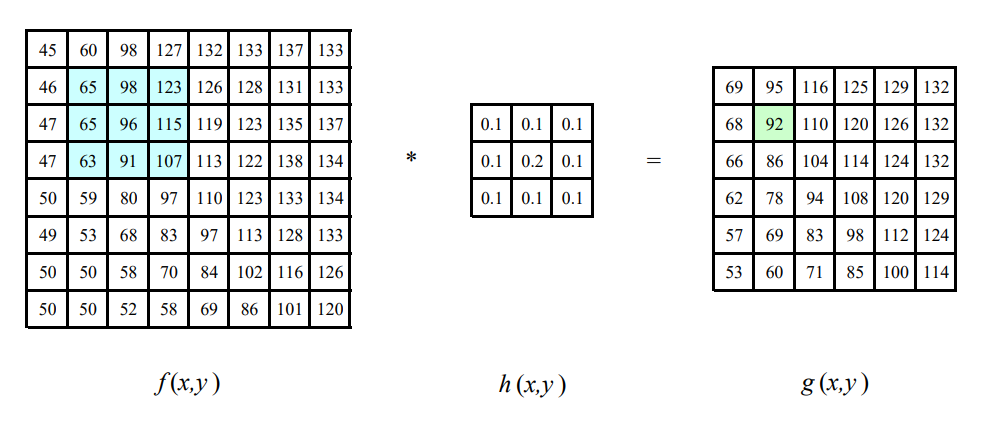
\includegraphics[width=0.8\textwidth]{EstadoDelArte/convolucion.png}
	\caption[Proceso de convolución en matrices]{Ejemplo de un proceso de convolución aplicado a una matriz (Fuente: Computer Vision: Algorithms and Applications, Richard Szeliski figure 3.10 \cite{szeliski})}
	\label{chap:Estado de la cuestion fig:CONV}
	\vspace{-5pt}
\end{figure}

Un claro ejemplo de este tipo de filtros es el suavizado. Permite suavizar la imagen y hacerla más homogénea al combinar cada pixel con sus vecinos. Este filtro permite reducir los valores atípicos reduciendo así el efecto del ruido. Pero también se puede dar el caso contrario en el que nos interese resaltar los pequeños detalles. Este filtro es conocido como \textit{Sharpening} y se basa en un filtro lineal de suavizado. A la imagen original se le resta las diferencias producidas por el suavizado y de esta forma se resaltan más los pequeños detalles de la imagen. Este proceso es conocido como \textit{unsharp masking} \cite{szeliski}.

\item \textbf{Filtros no lineales:} A pesar de que muchos de los filtros usados se pueden obtener de forma lineal, en muchas ocasiones se consigue un mejor rendimiento aplicando filtros no lineales. Tal y como su nombre indica, esta categoría engloba todos aquellos filtros que no se puedan expresar como una suma de diferentes argumentos. 

El beneficio de los filtros no lineales se puede ver al aplicar transformaciones que usen por ejemplo la mediana. El cálculo de la mediana puede suponer una alta carga computacional frente al resto de filtros. Por eso se han desarrollado alternativas para mejorar su cálculo. Tales como \textit{$\alpha$-trimmed mean} \cite{alfa}.

Un buen ejemplo de filtro no lineal que emplee la mediana es la transformación a escala de grises. Se suele usar la mediana ya que es más robusta ante variaciones atípicas. En el reconocimiento de objetos es muy recomendable usar la escala de grises ya que se consigue una mejor detección de borde \cite{greyscale} y reduce la carga computacional al trabajar con una sola matriz (\textit{Black}) en lugar de tres (RGB). Existen múltiples algoritmos para transformar a escala de grises, aunque uno de los más empleados y que mejores resultados da para el reconocimiento de borde es \textit{Lightness color-to-greyscale conversión algorithm} \cite{greyscale}. Sin embargo, gracias a los avances en redes neuronales y a la mejoras computacionales los sistemas actuales no se ven tan limitados y por ello son capaces de trabajar con imágenes de alta resolución y los tres canales RGB.
\end{itemize}


\subsubsection*{Detección de bordes}
Los bordes son el pilar fundamental de la visión artificial. Representan la separación entre diferentes objetos y definen sus formas. En una imagen, un borde se define como un salto de la intensidad de los pixeles.

En la práctica, estos cambios no son tan bruscos, sino que se producen gradualmente a lo largo de varios pixeles. Por ello no son tan fáciles de detectar y suelen aparecer bordes residuales producidos por ruido y errores en la imagen. En la detección de borde existen dos claras vertientes, aquellos métodos que se basan en el gradiente y los que emplean el laplaciano.

\begin{itemize}
\item \textbf{Operadores basados en gradientes:} El gradiente de una función es la colección de todas las derivadas parciales en forma de vector. La dirección del vector es la de máximo crecimiento y su módulo es el valor de la pendiente \cite{khan}. Al aplicar este concepto a imágenes, podemos obtener para cada píxel un vector que indique la dirección en la que aumenta la intensidad y su módulo. Analizando los gradientes obtenidos con la ayuda de máscaras, podemos encontrar los bordes ya que se producen por un cambio brusco de intensidad.

Existen varios algoritmos basados en el gradiente, aunque algunos de los más conocidos son el de Robert, Prewitt y el de Sobel. La diferencia entre estos son las máscaras a aplicar. Robert es un operador diferencial discreto con una matriz de 2x2, mientras que Prewitt y Sobel emplean dos matrices de 3x3. Se puede ver una comparativa de estos en la Figura \ref{chap:Estado de la cuestion fig:EDGE}.

El principal inconveniente de estos operadores es su forma de representar los bordes ya que están definidas por una franja de pixeles y además se ven bastante afectados por el ruido. Por ello existen algoritmos basados en la segunda derivada (laplaciano) para delimitar más la región de borde y obtener una mayor precisión.
\end{itemize}

\begin{figure}[ht]
	\centering
	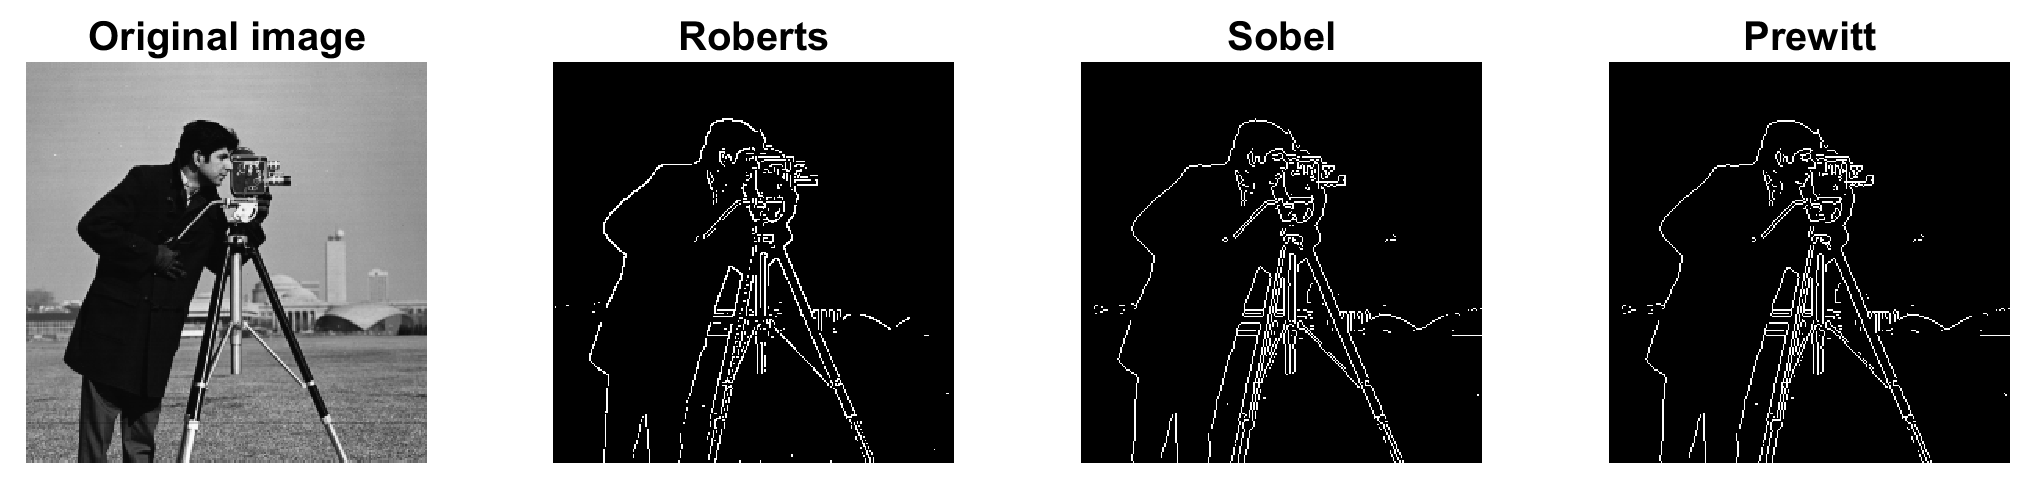
\includegraphics[width=0.9\textwidth]{EstadoDelArte/edge_detection_comparative.png}
	\caption[Comparativa de algoritmos de detección de borde]{Comparativa de algoritmos de detección de borde (Fuente: Ejemplo 		de MATLAB con imágenes de stock)}
	\label{chap:Estado de la cuestion fig:EDGE}
	\vspace{-5pt}
\end{figure}

\begin{itemize}
\item \textbf{Operadores basados en laplacianos:} Emplean la segunda derivada para obtener una mejor representación del borde y mayor robustez frente al ruido. Pero a cambio, requieren de una mayor carga computacional \cite{edgecomp}.

Existen múltiples algoritmos basados en el laplaciano, pero el más importante y usado es Canny. Esto es debido a su alto nivel de precisión y eficiencia. Asimismo, debido a su popularidad, han surgido múltiples variantes del algoritmo de Canny para perfeccionar la detección de borde.

El algoritmo de Canny se realiza en tres etapas. El primer paso es aplicar un filtro gaussiano para suavizar la imagen y evitar falsos bordes producidos por ruido en la imagen. A continuación, se calcula el gradiente de cada punto con su dirección y módulo. En este paso se intenta encontrar todos los bordes posibles de la imagen, pero con una diferencia respecto a los algoritmos anteriores, en este caso solo se queda con los máximos locales, convirtiendo así los bordes en líneas más nítidas y sin el efecto rampa. Por último, se hace un filtrado para eliminar los bordes innecesarios. Para ello se aplica un doble umbral sobre los gradientes y seguido por un rastreo de histéresis. Este elimina todos aquellos posibles puntos que no estén conectados a un borde. Se pueden observar los resultados en la Figura \ref{chap:Estado de la cuestion fig:EDGE2}.
\end{itemize}

\begin{figure}[ht]
	\centering
	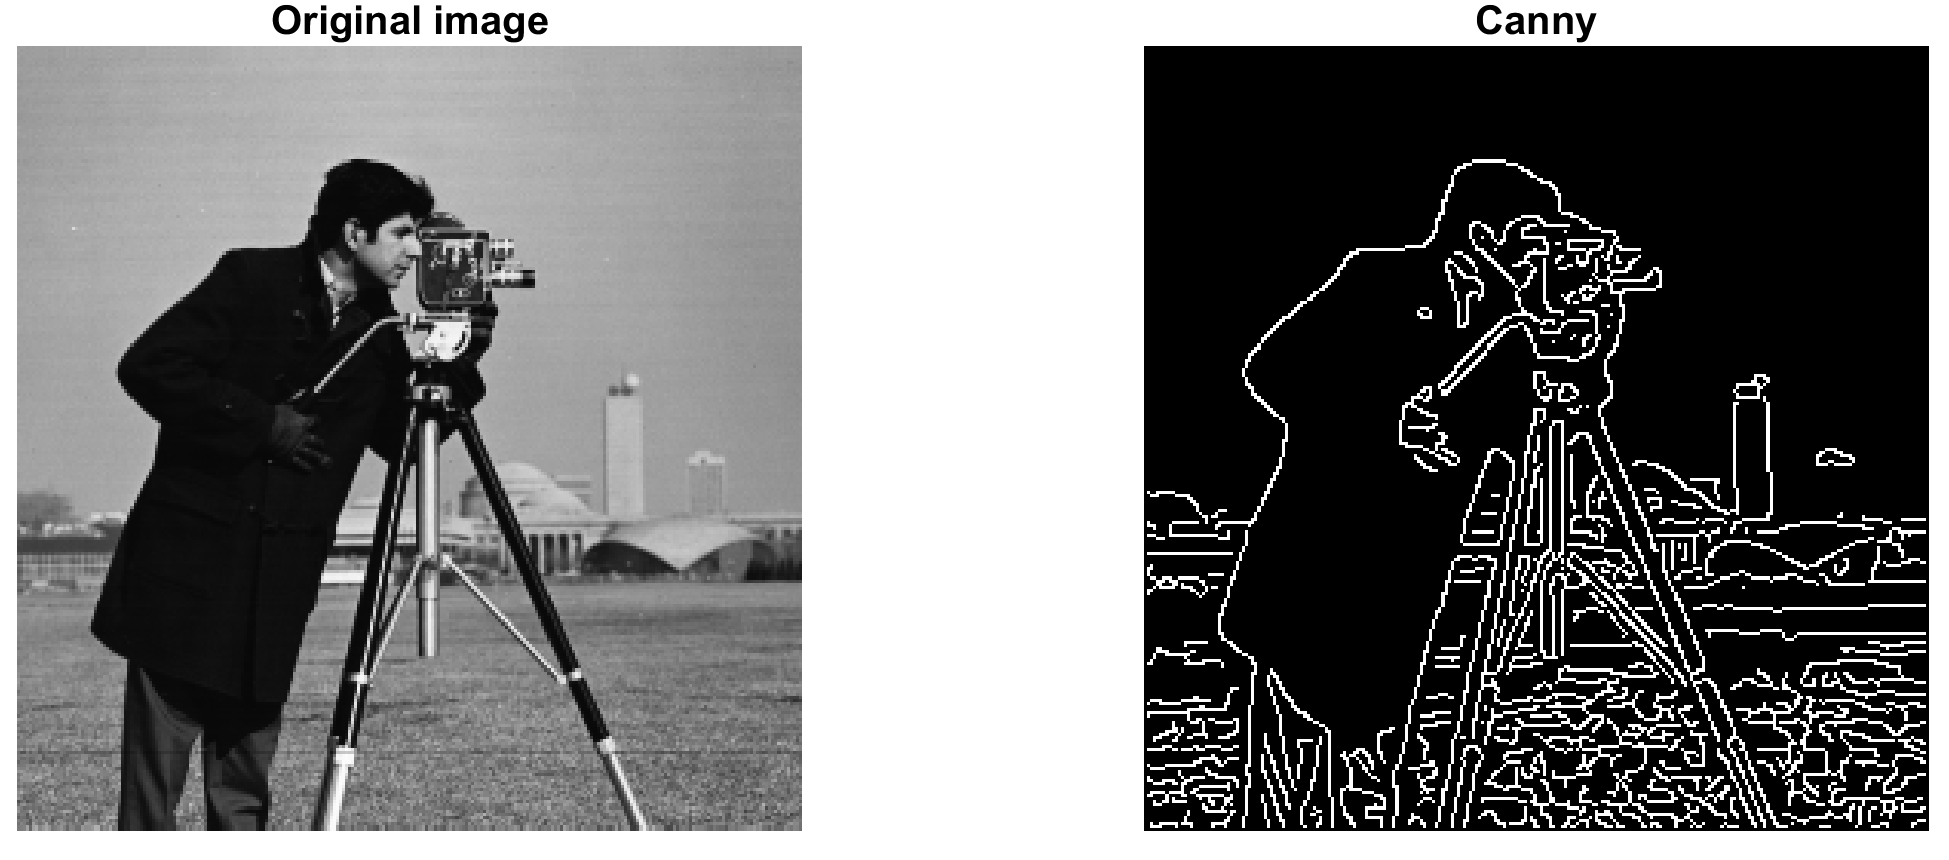
\includegraphics[width=0.8\textwidth]{EstadoDelArte/edge_detection_canny.png}
	\caption[Detección de borde por algoritmo de Canny]{Detección de borde por algoritmo de Canny (Fuente: Ejemplo de MATLAB con imágenes de stock)}
	\label{chap:Estado de la cuestion fig:EDGE2}
	\vspace{-5pt}
\end{figure}
	
\subsubsection*{Detección de formas}
Tras procesar la imagen y aplicar los algoritmos de detección de borde, se puede comenzar a analizar la escena. El objetivo de esta etapa es reconocer líneas y formas para poder detectar la posición y orientación del objeto. De nuevo, existen múltiples algoritmos para solventar el problema de localización y determinación a partir de imágenes. En este documento solo se van a analizar dos, la transformada de Hough y \acs{ransac} ya que en múltiples ocasiones han demostrado su robustez y son dos de los algoritmos más extendidos.

\begin{itemize}
\item \textbf{Transformada de Hough:} Este algoritmo fue diseñado en 1972 por Richard Duda y Peter Hart \cite{hough} y se ha postulado como una de las mejores alternativas para el reconocimiento de formas geométricas primitivas. Entendiéndose estas como una curva o superficie que pueda ser expresada matemáticamente con tres parámetros \cite{hough}. Por ejemplo, una línea, circulo, elipse, etc.

Para poder identificar curvas o superficies, el algoritmo analiza cada punto de la imagen y hace pasar por este todos los patrones posibles. Para cada punto se almacena $\rho$, que representa la distancia mínima entre la recta a analizar y el origen de coordenadas, esta viene dada por una perpendicular a la recta. Y $\theta$ que es el ángulo del vector director de esa recta \cite{hough2}. Esto se puede ver gráficamente en la Figura \ref{chap:Estado de la cuestion fig:Hough}.

La transformada de Hough ha demostrado numerosas veces su gran robustez para detectar patrones y líneas, pero a pesar de ello, presente un gran inconveniente que impide que sea usada tan extensamente. Requiere de una alta carga computacional ya que debe analizar cada punto de la imagen y almacenar todas las posibles rectas/formas. Por ello, se han desarrollado multitud de variantes del algoritmo original con el fin de o mejorarlo o reducir su carga. Algunas de las variantes más notables son:

\begin{itemize}
\item \textit{\ac{rht}}: Se basa en el algoritmo original, pero con la peculiaridad de que no necesita analizar todos los puntos de la imagen. El algoritmo intenta seleccionar de forma aleatoria puntos que puedan formar parte de una posible curva. De esta forma, se reduce bastante la carga computacional.
	
\item \textit{\ac{pht}}: Parte del esquema de acumulación del algoritmo original, pero difiere en el método de selección del siguiente punto a analizar. Selecciona un subconjunto a analizar en el que se ha incluido puntos previamente detectados como borde. De esta forma se reduce notablemente la carga computacional.
		
\item \textit{\ac{ppht}}: Partiendo de la imagen original, se seleccionan puntos de forma aleatoria y se analizan antes de pasar al siguiente. Para cada punto se observa si puede formar parte de una línea o no y se decide en base a los resultados obtenidos por los anteriores puntos. La principal ventaja de este algoritmo es la capacidad de poder ser interrumpido en cualquier momento y aun así dar buenos resultados. Pero es bastante susceptible a dar falsos positivos producidos por ruido en la imagen.
\end{itemize}

\end{itemize}

\begin{figure}[ht]
	\centering
	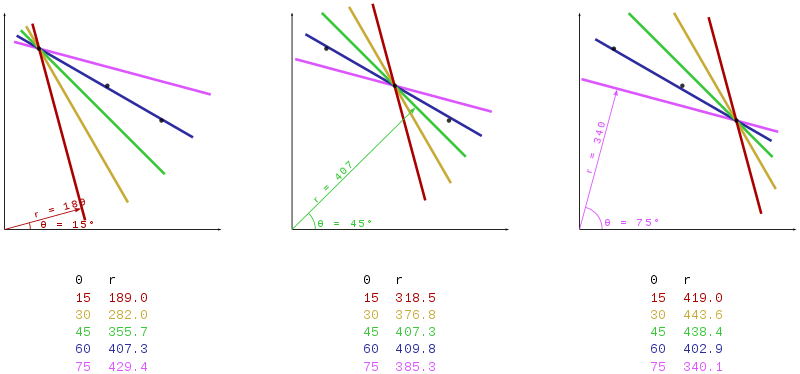
\includegraphics[width=0.7\textwidth]{EstadoDelArte/Hough_transform_diagram.png}
	\caption[Representación de la transforma de Hough]{Representación de la transforma de Hough (Fuente: \url{https://en.wikipedia.org/wiki/Hough_transform})}
	\label{chap:Estado de la cuestion fig:Hough}
	\vspace{-5pt}
\end{figure}

\begin{itemize}
\item \textbf{\textit{\acl{ransac}}:} También conocido como \acs{ransac}, se trata de un método matemático iterativo para encontrar los parámetros de un modelo matemático dentro de unos datos. Fue publicado por primera vez en 1981 por Fischler y Bolles y desde entonces se ha convertido en uno de los pilares de la visión artificial \cite{Fischler1981RandomSC}.

El método iterativo se puede separar en varias etapas que se repiten consecutivamente, tantas veces como se desee. Al aumentar el número de iteraciones, aumenta la probabilidad de detectar el objeto. Las etapas de cada iteración son:

\begin{itemize}
\item Selección de un subconjunto aleatorio sobre el que trabajar. Se conocen como \textit{inliers hipotéticos}.
\item  Basándose en el subconjunto, se monta un modelo sobre este.
\item Se comprueba la robustez del modelo contrastando contra el resto de los datos.
\item Si suficientes puntos se han clasificado como parte del modelo, este es válido.
\end{itemize}

En la siguiente iteración se partirá de este modelo y se intentará mejorar la detección de este.

Este algoritmo a pesar de ser muy preciso presenta una gran desventaja. Solo es capaz de contrastar la imagen frente a un modelo dado, por ello solo es capaz de detectar un tipo de objeto. Por ello se han desarrollado alternativas como \ac{r-ransac}.
\end{itemize}

\subsection{Redes neuronales convolucionales}
\label{chap:Estado de la cuestion sec:Procesado de la imagen subsec:Redes neuronales convolucionales}
La idea del aprendizaje automatizado/aprendizaje profundo/inteligencia artificial  no es novedosa, ya en 1955 IBM formó un grupo centrado en el reconocimiento de patrones supervisado por Nathaniel Rochester. Para ello, decidieron simular el funcionamiento de las neuronas con un ordenador IBM 704 \cite{Rochester}. Y aunque estos conceptos no suenan novedosos, es importante repasar los conceptos principales para poder entender las técnicas de aprendizaje automatizado \citep{alom2018history}.

En función del tipo de aprendizaje que se vaya a realizar, los tipos de inteligencias artificiales se pueden separar en 4 categorías:

\begin{itemize}
\item Aprendizaje supervisado: la información de la que se va a aprender ha sido preparada y etiquetada. Es un trabajo largo y tedioso, pero le permite a la inteligencia saber qué es lo que debe aprenderse.
\item Aprendizaje semi-supervisado: Tal y como su nombre indica, en este caso no toda la información ha sido preparada y etiquetada. 
\item Aprendizaje no supervisado: La información no ha sido preparada de ninguna forma y es el trabajo de la inteligencia el de entender la información y distinguir qué es lo que se desea aprender.
\item Aprendizaje por refuerzo: es un área del aprendizaje automático inspirada en la psicología conductista. La inteligencia debe de decidir que acciones tomar en un entorno y en función de sus decisiones recibirá una recompensa.
\end{itemize}

Qué tipo de aprendizaje usar depende del tipo de problema que se intente aprender. En este proyecto se va a emplear el aprendizaje supervisado. Para ello se emplearán imágenes previamente etiquetadas para que una red neuronal pueda aprender de ellas.

Desde la década de los cincuenta han surgido múltiples algoritmos para intentar simular el comportamiento de las neuronas y así poder alcanzar el objetivo de aprendizaje automatizado/profundo. Pero no fue hasta 1989 que surgió el concepto de Red Neuronal Convolucional impulsado por Yann LeCun. Yann desarrolló una de las primeras redes capaces del auto aprendizaje diseñada para reconocer la escritura a mano \cite{LeCun}. LeCun destacó por el uso de la convolución y fue uno de los primeros en obtener unos resultados positivos con este método.

En 2012 un grupo de investigadores dirigido por Alex Krizhevsky consiguieron obtener el menor error de clasificación visto hasta la fecha sobre las 1.2 millones de fotos de ImageNet con 1000 clases diferentes \cite{AlexNet}. Fue gracias a esta hazaña que empezó a crecer un gran interés por las redes neuronales convolucionales frente al resto de alternativas. Estas nuevas redes se basan en el principio de convolución, el cual ha sido explicado en la \autoref{chap:Estado de la cuestion sec:Procesado de la imagen subsec:Filtros, detección de borde y detección de formas}. La convolución se caracteriza por ser un proceso completamente lineal, esto es lo que ha permitido el desarrollo de estas redes y que puedan aprender tan fácilmente. En la actualidad este tipo de redes son las más comunes para el análisis de imágenes y su uso está ampliamente extendido.

Dentro del procesado de imágenes por aprendizaje profundo se distinguen dos categorías de redes en función de su objetivo:

\begin{itemize}
\item Clasificadores: son capaces de identificar un objeto en una imagen. Pueden ser entrenados para identificar una gran cantidad de objetos, pero tienen la desventaja de que solo pueden detectar un objeto por imagen. Además, solo indican su presencia, no su posición. Uno de los clasificadores más conocidos es AlexNet, la red neuronal diseñada por Alex Krizhevsky y mencionada anteriormente. Se muestra su estructura en \autoref{chap:Estado de la cuestion fig:AlexNet}.

\begin{figure}[ht]
	\centering
	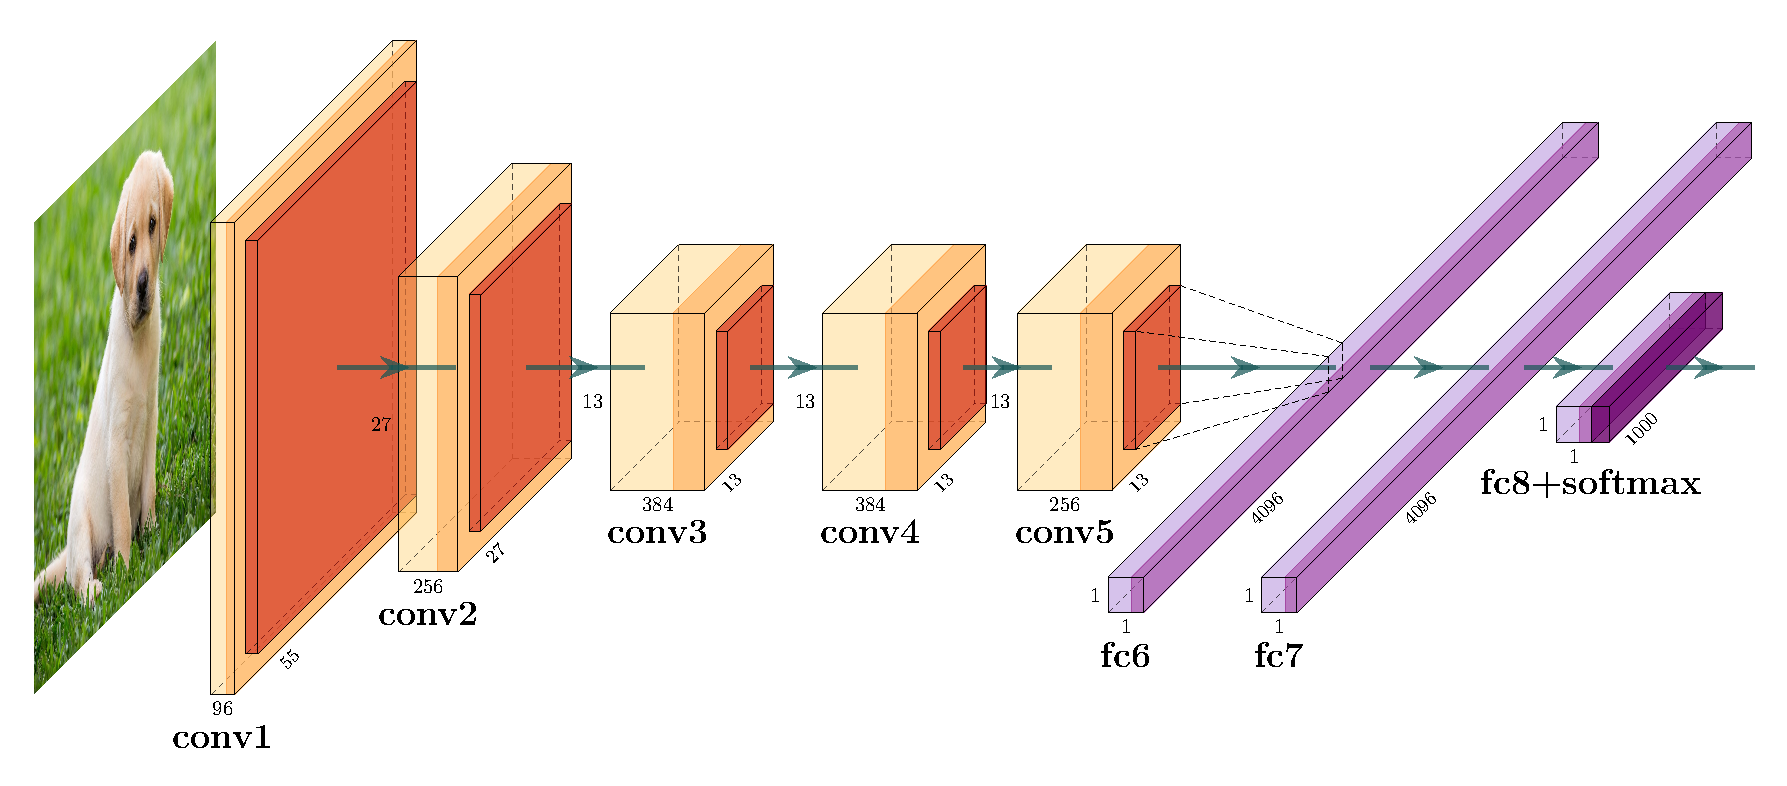
\includegraphics[width=0.9\textwidth]{EstadoDelArte/AlexNet.pdf}
	\caption[Estructura de AlexNet]{Representación de la estructura de AlexNet \cite{AlexNet}}
	\label{chap:Estado de la cuestion fig:AlexNet}
	\vspace{-5pt}
\end{figure}

En los últimos años los clasificadores han vivido una gran evolución y desarrollo y en parte esto es debido a la competición de ImageNet. Todos los años, investigadores de todo el mundo compiten por intentar obtener el mejor resultado al intentar clasificar millones de imágenes y mil clases. En la actualidad ImageNet cuenta con más de 14 millones de imágenes de alta resolución para ser clasificadas en mil clases. A continuación, se muestra en la \autoref{chap:Estado de la cuestion fig:ImageNet} el avance de las redes en este área analizando el error cometido por estas en ImageNet. Como referencia también se ha añadido el error medio cometido por los humanos. Se puede observar que algunas de las redes más modernas ya son capaces de superar al ojo humano en estas pruebas.

\begin{figure}[ht]
	\centering
	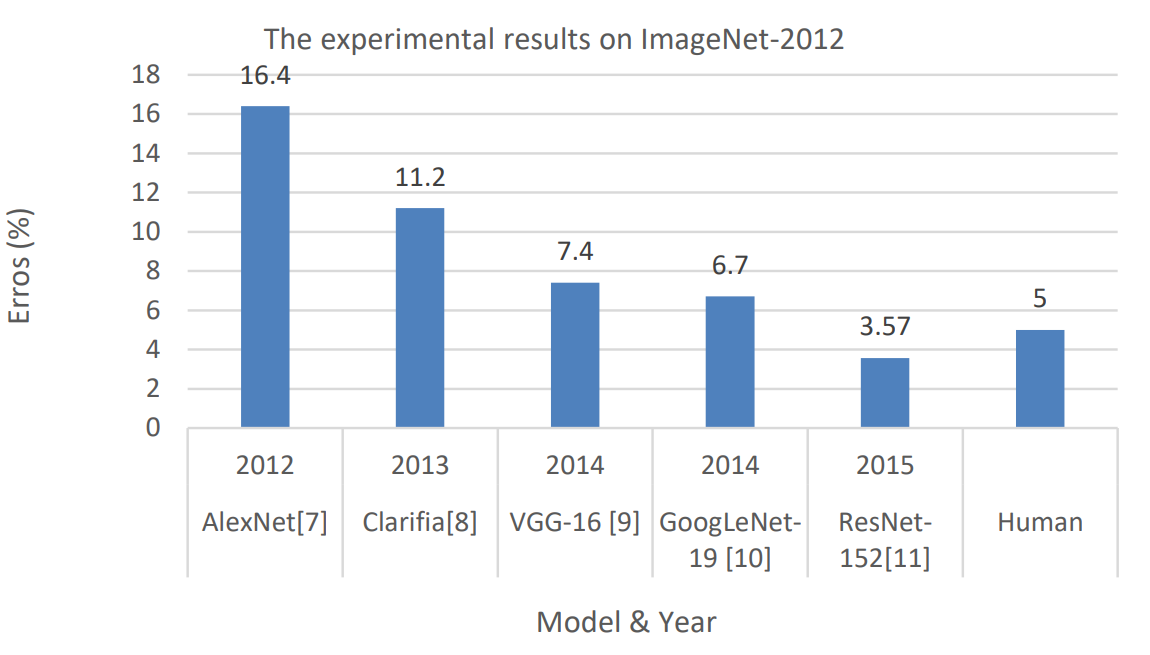
\includegraphics[width=0.7\textwidth]{EstadoDelArte/ImageNet.png}
	\caption[Errores cometidos en ImageNet en los últimos años]{Errores cometidos en ImageNet en los últimos años (Fuente: The History Began from AlexNet: A Comprehensive Survey on Deep Learning Approaches \cite{alom2018history}}
	\label{chap:Estado de la cuestion fig:ImageNet}
	\vspace{-5pt}
\end{figure}


\item Detectores de objetos: se basan en los principios de los clasificadores pero por medio de diferentes herramientas son también capaces de localizar el objeto en la imagen. Además, pueden identificar y detectar múltiples objetos en una misma imagen. En la actualidad existe una gran variedad de estructura y métodos para la detección de objetos, pero en este proyecto solo se van a analizar y emplear algunos de los más populares:

\begin{itemize}
\item \textit{\ac{r-cnn}}:Se basan en el principio de propuesta de regiones frente a sistemas empleados previamente conocidos como ventana flotante. Este sistema consiste en correr un clasificador barriendo todas las posibles secciones de una imagen y con diferentes tamaños. Como este proceso es muy costoso a nivel computacional y lento, \acs{r-cnn} propone usar un sistema que proponga un máximo de 2000 regiones a estudiar basándose en colores y formas fácilmente reconocibles. De esta forma se reduce bastante la carga, pero manteniendo un buen nivel de confianza y precisión.

\item \textit{\ac{faster-r-cnn}}: Al igual que \acs{r-cnn} se basan en el principio de propuesta de regiones pero difiere de este en el método para proponer dichas regiones de interés. En este método, la propia red neuronal se encarga de analizar la escena y decidir qué regiones debe considerar de interés. Esto resulta en una red bastante más rápida, aunque puede ser menos precisa que \acs{r-cnn}.

\item \textit{\ac{yolo}}: Es una de las técnicas más actuales y prósperas. Como su nombre indica, se caracteriza porque la imagen solo se pasa una vez por el clasificador y una capa convolucional se encarga de predecir la clase de objeto detectado y su posición. Este tipo de redes se caracterizan por ser extremadamente rápidas, aunque son incapaces de igualar la precisión de \acs{r-cnn}.
\end{itemize}
\end{itemize}


\section{Robótica industrial}
\label{chap:Estado de la cuestion sec:Robótica industrial}
El término robot se remonta hasta 1921 donde por primera vez se introdujo en la obra de teatro R.U.R (Rossum’s Universal Robots) obra del novelista y autor checo Karel Čapek. La palabra deriva de \textit{robota} que en checo significa fuerza del trabajo o servidumbre \cite{robotica}. En la actualidad es un término aceptado y conocido por toda la sociedad, empleado para designar a cualquier “máquina o ingenio electrónico programable que es capaz de manipular objetos y realizar diversas operaciones” (definición de robot según la RAE).

Actualmente los robots representan una gran parte de la fuerza de trabajo industrial. Se presentan en una gran variedad de configuraciones diferentes para cumplir diferentes objetivos, aunque una de las configuraciones más destacadas son los brazos robóticos. Tal y como su nombre indica, se asemejan a brazos de forma que tienen múltiples articulaciones sobre las que rotar para poder moverse en todas las direcciones y orientaciones posibles. 

Estos robots se pueden clasificar en función de diversas categorías:
\begin{itemize}
\item Por su función. Para ello se han desarrollado diferentes efectores que les permiten realizar tareas tan simples como \textit{Pick and Place} hasta tareas más exigentes como soldar.
		
\item Por su forma. Esta muchas veces se ve determinada por la función que debe desarrollar el brazo, así como el entorno en el que debe trabajar. Aunque a grandes rasgos se pueden distinguir dos tipos, fijos y móviles. Como sus nombres indican, esto depende de la capacidad del robot para moverse libremente.
		
\item Por el sistema de control. Los robots se pueden controlar por control manual, a distancia, mediante programación o con un sistema de aprendizaje por refuerzo.
		
\item Por el modelo de control de la planta. Una planta industrial dotada de numerosos robots tiene dos formas de ser controlada. Se puede tener un sistema de control independiente para cada robot, esto simplifica la creación de la planta, pero dificulta su manejo. O puede contar con un complejo sistema de interconexión entre las diferentes etapas de la planta. Un buen ejemplo de este tipo de sistemas de control es SCADA (Supervisory Control And Data Acquisition) \cite{SCADA}.
\end{itemize}

\begin{figure}[h]
	\centering
	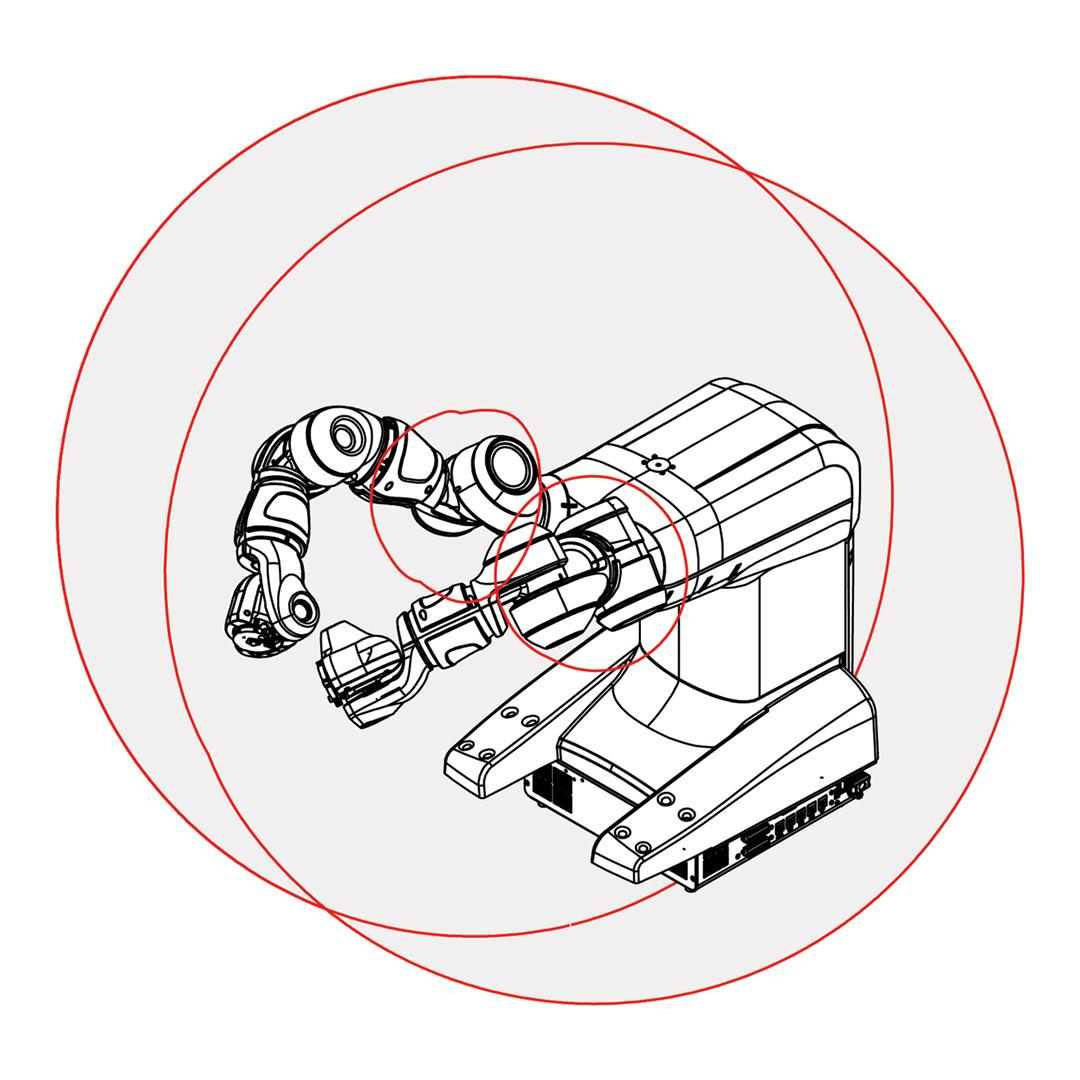
\includegraphics[width=0.6\textwidth]{EstadoDelArte/IRB1400.jpg}
	\caption[Brazo robótico IRB 1400 YuMi]{Brazo robótico IRB 1400 YuMi empleado en el proyecto con su rango de acción \cite{YuMi}}
	\label{chap:Estado de la cuestion fig:IRB1400}
	\vspace{-5pt}
\end{figure}

Como ya se ha explicado previamente, el objetivo de este proyecto es el desarrollo de un sistema capaz de localizar y capturar piezas para la preparación de un pedido. Este tipo de sistemas son conocidos como configuraciones \textit{Pick and Place} y son ampliamente usadas en la industria. Estos sistemas suelen estar constituidos por un brazo robot, una cámara y una unidad de procesamiento para analizar las imágenes. En función de los objetos que deben transportar, estos varían su forma de coger los objetos y sus cabezales.

Un buen ejemplo de la importancia de estos sistemas es \textit{Amazon Robotics Challenge}. Con el fin de mejorar los sistemas actuales y de buscar a los mejores en el sector, Amazon ha creado una competición entre alumnos universitarios para desarrollar el mejor sistema \textit{Pick and Place} \cite{amazon}. Estos sistemas se basan en redes neuronales muy avanzadas y desarrolladas tales como RefineNet \cite{amazon}.

  \chapter{Metodología de trabajo}
\label{chap:Metodologia de trabajo}
\Abstract{Para poder desarrollar w innovar es necesario primero definir una estructura base sobre la que edificar. Y se debe determinar un plan a seguir que sirva de guía.}

\section{Motivación}
\label{chap:Metodología sec:Motivación}
La industria avanza a un ritmo constante y cada día es más necesario la implantación de sistemas robóticos para poder llevar a cabo tareas que los humanos no podemos desarrollar o que presentan una elevada tasa de errores humanos o tienen un elevado nivel de peligrosidad. Al dotar a estos sistemas de inteligencia y un sistema de visión artificial, se consigue que se pueda adaptar mejor al entorno y se evite tener que re-programar los robots con cada cambio de las condiciones de operación. Avanzamos hacia una sociedad en la que los robots serán la principal mano de obra y para llegar a ese objetivo es necesario invertir y desarrollar más los sistemas actuales. Por ello se ha propuesto como proyecto la integración de un sistema de visión artificial en un robot industrial. Con este proyecto se podrá modernizar las instalaciones del Grupo Antolín\textsuperscript{\textregistered} y aumentar las capacidades de la línea de montaje y ensamblaje actual.

\section{Objetivos}
\label{chap:Metodología sec:Objetivos}
Este trabajo parte de un proyecto actualmente en desarrollo con un sistema de visión artificial ya desarrollado e implantado. Desgraciadamente la implantación actual presenta limitaciones así como una tasa de error superior a los requisitos planteados por el Grupo Antolín.

Para poder superar las limitaciones actuales se ha planteado el desarrollo de un nuevo sistema que debe de mejorar las capacidades de identificación y detección de las piezas así como poder determinar el punto de agarre óptimo. El sistema debe de ser modular de forma que se pueda adaptar fácilmente a nuevas piezas. Y con el fin de que el robot tenga la mayor posibilidad de coger la pieza, también se debe de determinar el vector normal al punto de agarre. Por último, se pide que sea independiente del resto del proyecto de forma que pueda ser fácilmente manejado, modificado y actualizado.

Con el fin de cumplir dichos requisitos se deben plantear unos objetivos de corto, medio y largo alcance a seguir durante todo el desarrollo del trabajo:

\begin{itemize}
	\item Desarrollo de una base de datos sintética:
	\begin{itemize}
		\item Investigación y prueba de diferentes sistemas/herramientas (bpi, zpi Zumo labs y Blenderproc).
		\item Obtención de primeras imágenes RGB y de profundidad.
		\item Obtención de imágenes de profundidad, mapa de normales, identificación de las piezas, mapas de segmentación, etc.
		\item Introducción de aleatoriedad y repetibilidad al sistema.
		\item Generación de un \textit{Pipeline} para la automatización del proceso.
		\item Introducción de ruido en las imágenes para mejorar la robustez.
	\end{itemize}
	\item Desarrollo de una base de datos real complementaria tanto para la fase de entrenamiento como evaluación del sistema.
	\item Desarrollo de las nuevas redes neuronales:
	\begin{itemize}
		\item Investigación y pruebas de diferentes sistemas/herramientas (YOLO, MobilNet, redes regresoras, etc).
		\item Planteamiento y definición de la estructura modular a desarrollar. Una primera red para la detección de piezas, seguida de una red para la detección de zonas de intereses con probabilidad de ser el punto de agarre óptimo. Y finalmente un una red neuronal del tipo regresor para la determinación del punto de agarre. 
		\item Primeros desarrollos independientes de las partes modulares del sistema
		\item Desarrollo y corroboración del conjunto modular
		\item Creación del sistema de evaluación tanto del conjunto como de las partes modulares del sistema
		\item Entrenamiento y evaluación de todo el sistema con diferentes configuraciones y bases de datos.
		\item Comparativa y determinación del sistema óptimo.
		\item Implantación del nuevo sistema de visión artificial
	\end{itemize}
\end{itemize}

\section{Arquitectura del sistema}
\label{chap:Metodología sec:Arquitectura}
El sistema se compone de tres elementos claves: un robot industrial para poder interactuar con las piezas, una cámara RGB-D para la captura de imágenes y Python para el procesamiento de las imágenes y la toma de decisiones. Es necesario que estos tres elementos funcionen correctamente y estén comunicados entre sí. La arquitectura básica se puede ver en \autoref{chap:Metodología fig:Arq1}

\begin{figure}[ht]
	\centering
	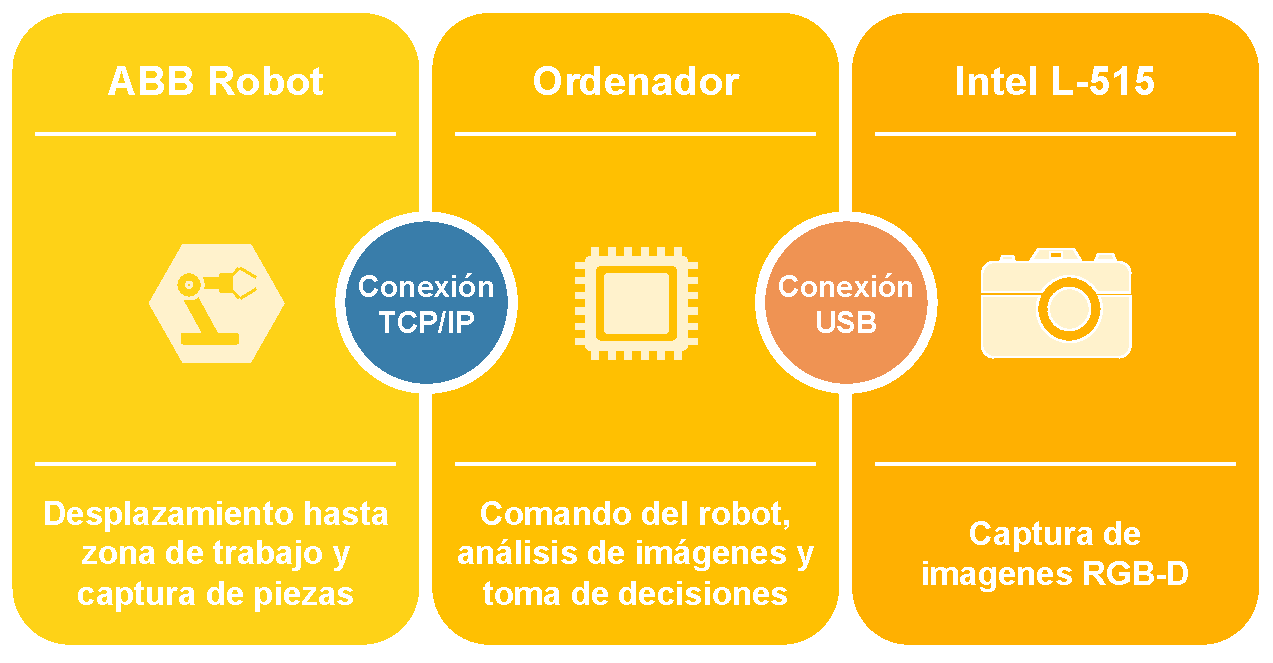
\includegraphics[width=0.9\textwidth]{Metodologia/Arquitectura.pdf}
	\caption{Esquema de la arquitectura del sistema}
	\label{chap:Metodología fig:Arq1}
	\vspace{-5pt}
\end{figure}

A continuación, se va a detallar todo el proceso desde el arranque del sistema hasta el final del mismo y se analizarán cada una de las etapas que constituyen el proceso. Este se puede ver gráficamente en \autoref{chap:Metodología fig:Arq2}. El sistema debe compenetrase con los sistemas actuales los cuales diseñan los pedidos que se deben de preparar y ensamblar. Estos pedidos se reciben y se procesan para establecer qué piezas se desean y en que orden deben de ser recogidas por medio de un proceso cíclico.

Una vez procesado el pedido y establecida la primera pieza a recoger se debe de desplazar el robot a la zona de trabajo y prepararse  para la captura de dicha pieza. Una vez reubicado el robot, un sistema de cámaras capturará la escena para determinar la posición de la pieza/piezas que se desean capturar frente a la posición del robot. Esta imagen es analizada por el sistema de visión artificial que se encargará de "en primera instancia" identificar las piezas para entre ellas poder centrarse solo en las que se desea capturar. A continuación, si se trata de una pieza de dimensiones grandes se analizará más en profundidad para determinar los posibles puntos de agarre. Y una vez determinados estos puntos de agarre un regresor determinará el centro exacto de dichos puntos de agarre así como el vector normal a dicho punto (dirección que debe emplear la muñeca del robot para capturar la pieza). Si por el contrario se trata de una pieza de dimensiones reducida se empleará el centro de la pieza como punto de agarre.

Esta información es transmitida al robot permitiéndole así poder capturar la pieza y depositarla en la cesta del pedido. Para ello este se deberá aproximar a la pieza seleccionada siguiendo en la medida de lo posible la trayectoria normal determinada. Al aproximarse a la pieza también deberá reducir la velocidad de operación para evitar colisionar.

\begin{figure}[ht]
	\centering
	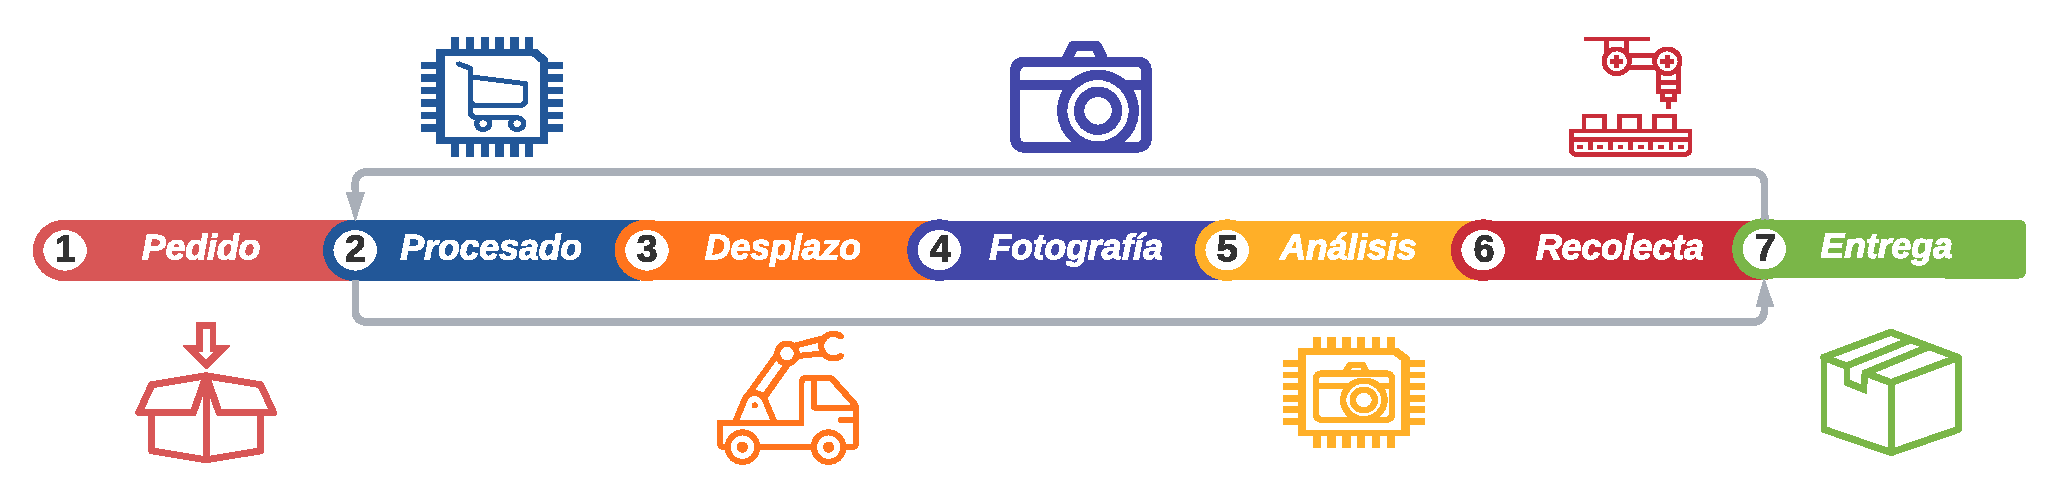
\includegraphics[width=1\textwidth]{Metodologia/Esquema arquitectura.pdf}
	\caption{Diagrama de las etapas del sistema}
	\label{chap:Metodología fig:Arq2}
	\vspace{-5pt}
\end{figure}

\section{Herramientas}
\label{chap:Metodología sec:Herramientas}
\begin{itemize}
	\item Cámara Intel RealSense L515 \cite{IntelL515} y Wrapper de Python para Intel Realsense \cite{SDK}.
	\item Ordenador con los siguientes SO/paquetes/programas:
		\begin{itemize}
			\item Ubuntu 20.04 LTS
			\item Blender 2.93.5
			\item BlenderProc 2.0 (Blender API)
			\item PyTorch 1.10.1
			\item Tensorflow 2.7.0
			\item CUDAToolkit
			\item Python 3.8 o superior
			\item Conda ó miniconda
		\end{itemize}
\end{itemize}

\section{Cronograma}
\label{chap:Metodología sec:Cronograma}
La planificación del proyecto permite establecer un orden a seguir. No solo da estructura al proyecto, también ayuda a los desarrolladores a estructurar sus ideas. Es por ello que es vital y necesario establecer guías, objetivos e hitos a seguir.

\begin{table}[htbp]
  \centering
  \caption{Cronograma del proyecto}
    \begin{tabular}{p{16.5em}cccc}
    \rowcolor[rgb]{ .251,  .251,  .251} \multicolumn{1}{c}{\textcolor[rgb]{ 1,  1,  1}{\textbf{Descripción del hito}}} & \multicolumn{1}{c}{\textcolor[rgb]{ 1,  1,  1}{\textbf{Categoría}}} & \multicolumn{1}{c}{\textcolor[rgb]{ 1,  1,  1}{\textbf{Progreso}}} & \multicolumn{1}{c}{\textcolor[rgb]{ 1,  1,  1}{\textbf{Inicio}}} & \multicolumn{1}{c}{\textcolor[rgb]{ 1,  1,  1}{\textbf{Días}}} \\
    \rowcolor[rgb]{ .949,  .949,  .949} \textbf{MVP} &       &       &       &  \\
    Estado de la Cuestión & Hito  & 100\% & 01/06/2021 & 14  \\
    \rowcolor[rgb]{ .949,  .949,  .949} Base de datos sintéticas v0.1 & Objetivo & 100\% & 15/06/2021 & 14  \\
    Detección puntos de agarre & Hito  & 100\% & 29/06/2021 & 7  \\
    \rowcolor[rgb]{ .949,  .949,  .949} Driver Intel RealSense v0.1 & Objetivo & 100\% & 06/07/2021 & 7  \\
    Regresor - Tensorflow v0.1 & Objetivo & 100\% & 13/07/2021 & 7  \\
    \rowcolor[rgb]{ .949,  .949,  .949} Evaluación regresor & Objetivo & 100\% & 20/07/2021 & 3  \\
    \textbf{Base de datos sintética v1.0} &       &       &       &  \\
    \rowcolor[rgb]{ .949,  .949,  .949} Introducción de Arucos & Objetivo & 100\% & 01/09/2021 & 21  \\
    Extracción y lectura de normales & Hito  & 100\% & 22/09/2021 & 7  \\
    \rowcolor[rgb]{ .949,  .949,  .949} Preparación de bases de datos & Objetivo & 100\% & 29/09/2021 & 21  \\
    Actualización a Blenderproc 2.0 & Hito  & 100\% & 20/10/2021 & 7  \\
    \rowcolor[rgb]{ .949,  .949,  .949} Replicabilidad & Objetivo & 100\% & 27/10/2021 & 7  \\
    Riqueza de escenarios& Hito  & 15\% & 03/11/2021 & 14  \\
    \rowcolor[rgb]{ .949,  .949,  .949} Generación de base de datos real & Objetivo & 0\% & 17/11/2021 & 7  \\
    \textbf{Visión artificial v1.0} &       &       &       &  \\
    \rowcolor[rgb]{ .949,  .949,  .949} Estado de la Cuestión & Hito  & 100\% & 01/12/2021 & 10  \\
    Arquitectura del sistema & Objetivo & 100\% & 11/12/2021 & 14  \\
    \rowcolor[rgb]{ .949,  .949,  .949} YOLO & Objetivo & 100\% & 25/12/2021 & 7  \\
    TINY YOLO & Objetivo & 100\% & 01/01/2022 & 7  \\
    \rowcolor[rgb]{ .949,  .949,  .949} Regresor & Objetivo & 15\% & 08/01/2022 & 30  \\
    \textbf{Evaluación} &       &       &       &  \\
    \rowcolor[rgb]{ .949,  .949,  .949} Tamaño del dataset sintético & Objetivo & 0\% & 14/02/2022 & 30  \\
    Comparativa con dataset real & Objetivo & 0\% & 16/03/2022 & 10  \\
    \rowcolor[rgb]{ .949,  .949,  .949} \textbf{Redacción} &       &       &       &  \\
    Anexo B & Objetivo & 100\% & 01/12/2021 & 20  \\
    \rowcolor[rgb]{ .949,  .949,  .949} Memoria & Objetivo & 15\% & 01/04/2022 & 50  \\
    \end{tabular}%
  \label{chap:Metodología tab:plan}%
\end{table}%

\begin{figure}[ht]
	\centering
	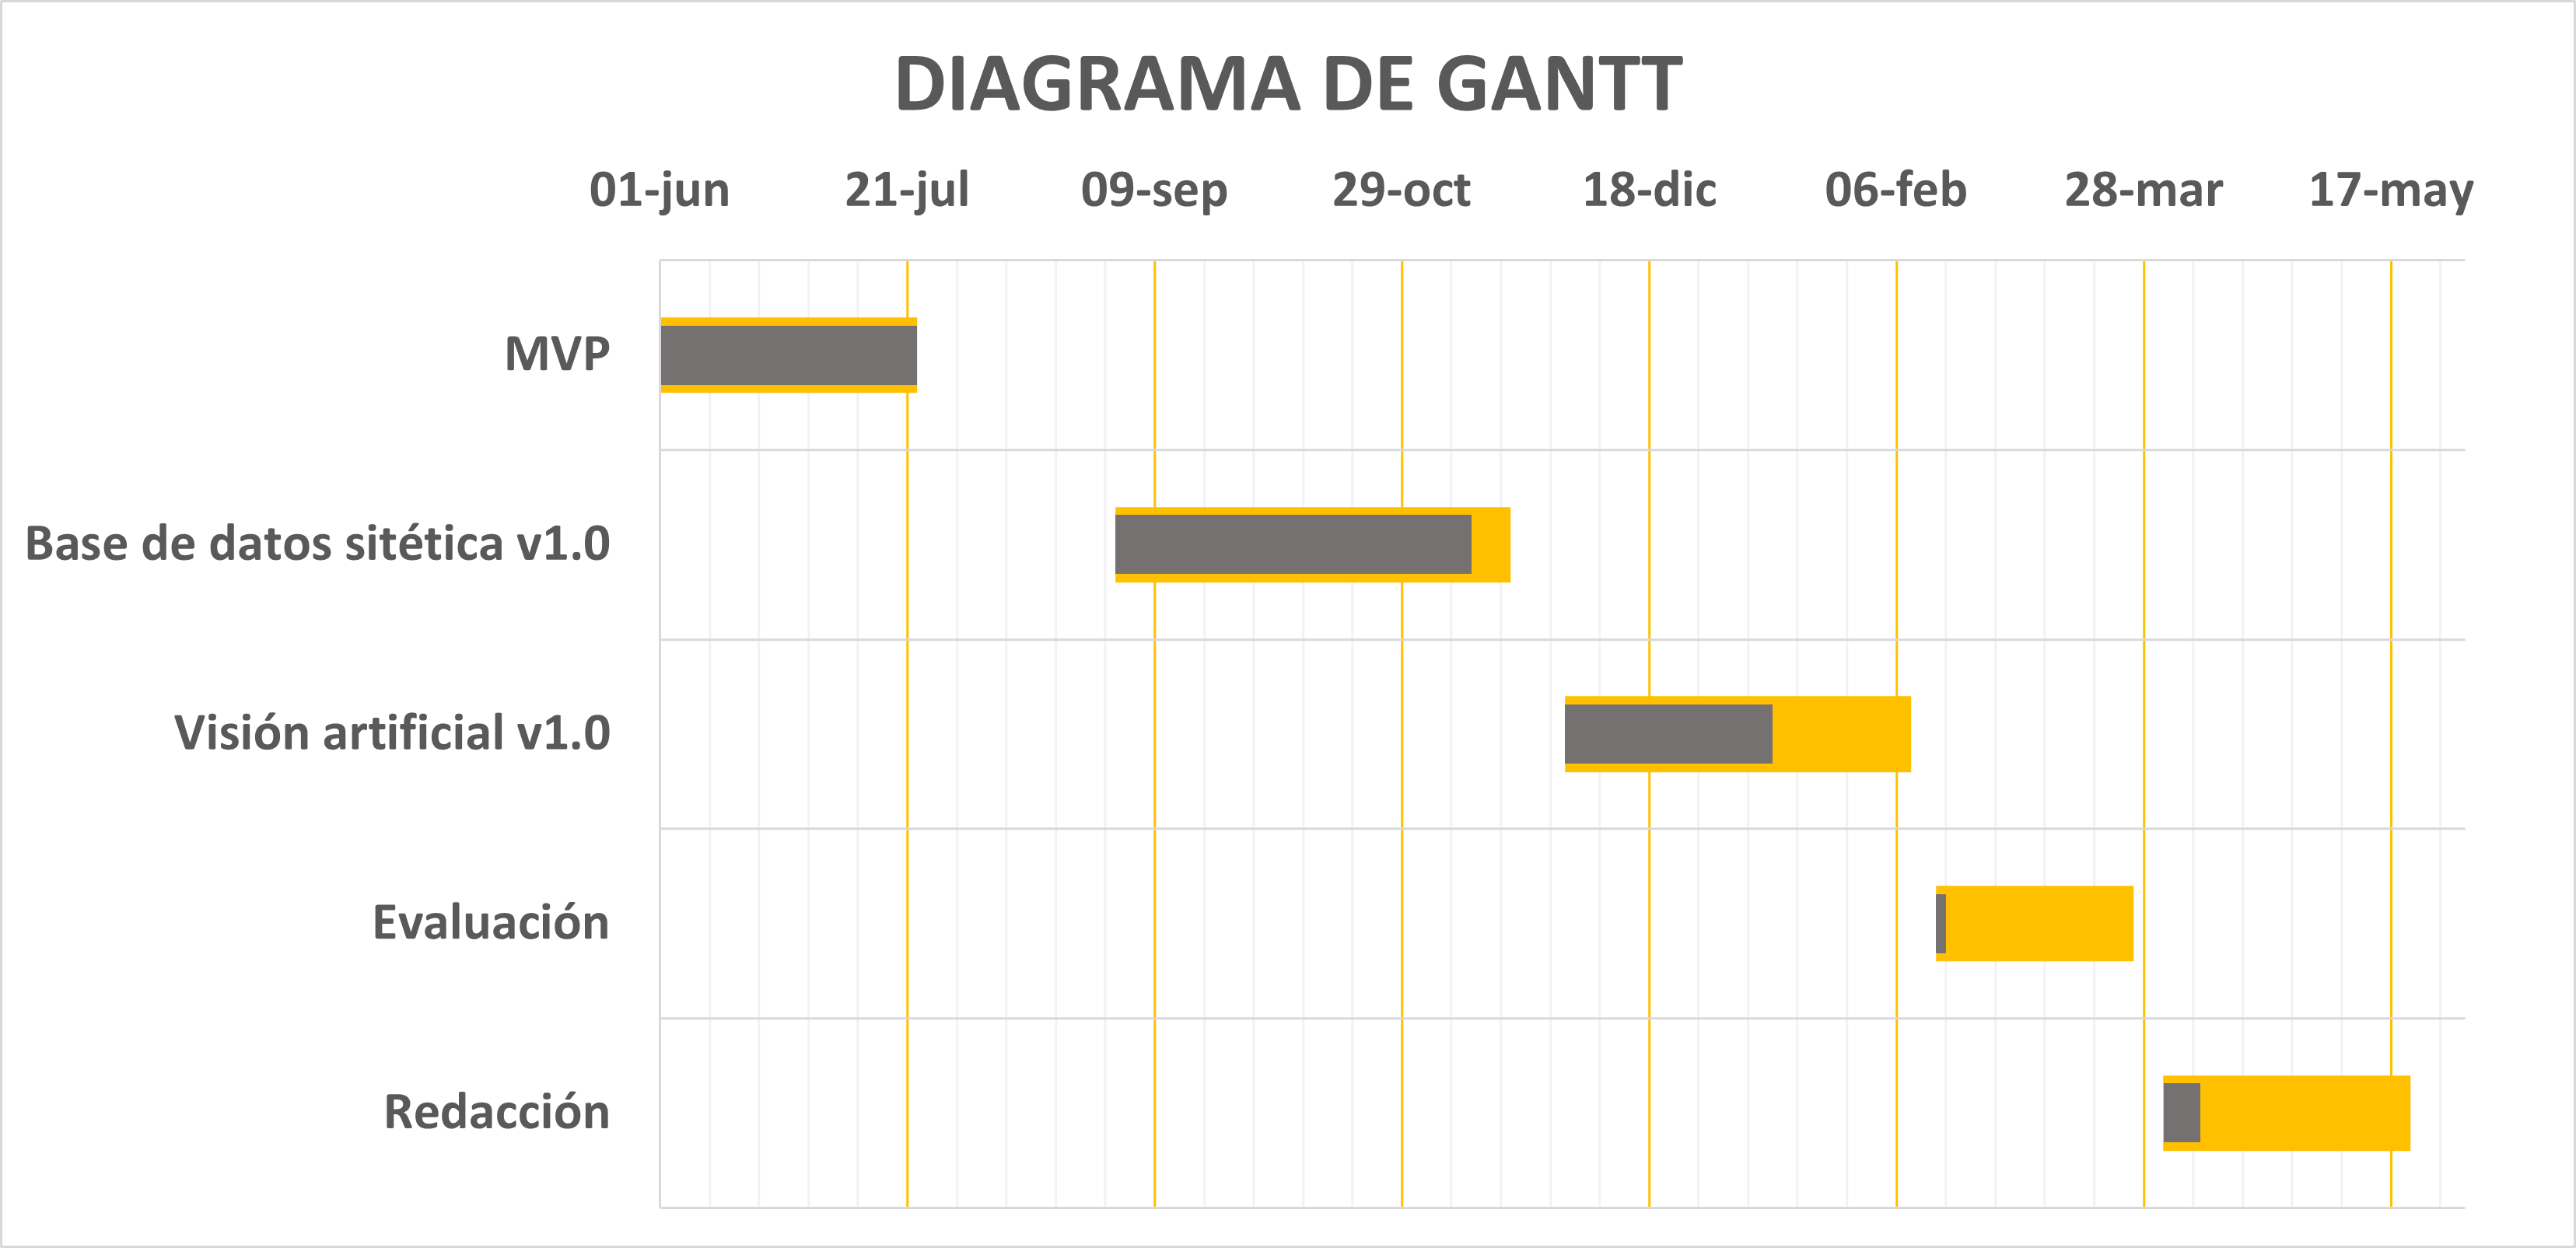
\includegraphics[width=1.0\textwidth]{Metodologia/Diagrama_de_gantt.png}
	\caption{Diagrama de gantt del proyecto}
	\label{chap:Metodología fig:Gantt}
	\vspace{-5pt}
\end{figure}
  \chapter{Generación de un dataset}
\label{chap:Generación de un dataset}
\Abstract{Un buen sistema de visión artificial requiere de un buen \textit{dataset}. En este capítulo se desarrollará y justificará la creación de un \textit{dataset} sintético que permita expandir las capacidades del sistema de visión artificial.}

Se entiende por \textit{dataset} a un conjunto de datos normalmente tabulados/organizados empleados en la ejecución de programas o algoritmos. El término \textit{dataset} es muy amplio y su funcionalidad y formato varía dependiendo del campo de desarrollo pero en este trabajo nos centraremos en una de las áreas donde mas se ha desarrollado el concepto, \textit{Machine Learning}. La capacidad de aprender de un modelo depende en primera instancia de la calidad del \textit{dataset}. Si este no tiene un formato correcto o no es capaz de asegurar la integridad de los datos entonces independientemente del modelo empleado el resultado sera desfavorable. Por lo tanto, la creación del \textit{dataset} es de vital importancia y debe de ser uno de los primeros pasos en el desarrollo de todo sistema basado en \textit{Machine Learning}.

Uno de los métodos mas comunes es la generación de forma manual del \textit{dataset}. Esto implica que un ser humano debe de categorizar, estructurar y definir el valor del dato. Se caracteriza por ser sencillo y rápido para \textit{datasets} pequeños pero presenta numerosos problemas cuando se requiere de datos complejos o de un tamaño elevado. Este proyecto entra dentro de esta categoría y es por ello que se ha creado un sistema de generación de datos que ha permitido automatizar y agilizar el proceso. A este tipo de \textit{datasets} creados por ordenador se les define como sintéticos. Sin embargo no se recomienda depender solo de \textit{datasets} sintéticos ya que estos no reflejan con total precisión la realidad. Es recomendable desarrollar un sistema que mezcle datos reales y sintéticos durante la fase de entrenamientos. Y emplear datos reales para la fase de validación ya que solo de esta forma se puede determinar la verdadera capacidad del modelo.

Pero antes de analizar los datos y las herramientas creadas para obtenerlos, es necesario entender que datos se desean obtener. Para ello se debe de entender el objetivo/problema del proyecto (\ref{chap:Metodología sec:Objetivos}), el agarre de piezas industriales de diferentes formas y tamaños. Este problema se puede dividir en etapas:

\begin{enumerate}
\item Generación del pedido: en función de la demanda y de los requisitos del cliente se debe de generar una lista con todos los componentes necesarios para cada pedido.
\item Estructuración del pedido: Las piezas necesarias se encuentran distribuidas en diferentes secciones y es por ello que se debe de crear un  que determine el orden de recolección de piezas optimo que reduzca el tiempo recolección.
\item Recolección de piezas: Se trata de un proceso iterativo que se debe de realizar para cada una de las piezas que constituyen el pedido.
\begin{itemize}
\item Desplazamiento hasta la pieza. Dependiendo de la configuración del robot este sistema variará, pero el objetivo siempre será el mismo. Trasladar el robot hasta la región donde se encuentra la pieza a recolectar con el fin de poder capturarla y situarla dentro de la región de alcance.
\item Detección de la pieza: aplicando algoritmos de detección se identificará la pieza que se desea recolectar. Dentro de una misma zona se detectarán numerosas instancias de una misma pieza. Se debe de escoger la pieza/piezas mejor ubicadas y con más probabilidad de éxito.
\item Punto de agarre: tras detectar la pieza se debe de determinar como se debe de agarrar la pieza. Para ello se debe de determinar el punto de agarre óptimo y el vector normal a dicho. Para las piezas pequeñas se puede emplear el centro de la pieza como punto de agarre. Sin embargo, para piezas más grandes este método no funciona ya que se trata de piezas irregulares que debido a su gran tamaño requieren de un buen agarre capaz de levantar el peso de la pieza. Por ello se debe de buscar zonas lisas sobre las que se pueda emplear una ventosa o superficies más complejas que permitan el uso de un cabezal \textit{soft-robotics}. Esto implica que la salida final del sistema debe de ser un punto de agarre y el vector normal a dicho punto que debe de seguir el brazo robótico.
\item Recolección de la pieza: se transfiere la información necesaria al robot para que este pueda recolectar la pieza a través del punto de agarre definido. El sistema de agarre a emplear dependerá del tpo de pieza.
\item Deposición y control de calidad: por último se debe de depositar la pieza dentro de la cesta que constituye el pedido. Y mediante el sistema de visión artificial se debe de comprobar que la pieza deseada ha sido correctamente depositada en la cesta.
\end{itemize}
\item Control de calidad y trazabilidad: antes de dar por finalizado en pedido se analiza por última vez para comprobar que todas las piezas necesarias se encuentran dentro de la cesta. Se registra en el sistema el pedido y toda la información necesaria para futura trazabilidad.
\item Traslado del pedido: una vez se da por finalizado el pedido este se debe de trasladar hasta la zona de ensamblaje para comenzar el proceso de montado.
\end{enumerate}

\section{Estructura del dataset}
\label{chap:Generación de un dataset sec:Estructura del dataset}
Una vez entendido el problema se puede determinar el tipo de datos que se necesitan y para este problema se puede observar que dependen en gran medida de la pieza. Por ello se debe de distinguir entre las piezas grandes y las piezas pequeñas. A continuación, se muestra la estructura estándar que deben de seguir las piezas pequeñas y grandes:

\noindent
\begin{itemize}[wide, nosep, labelindent = 0pt, topsep = 1ex]
\item[\textbf{Piezas pequeñas}]
\item Imagen en formato ".png" de toda la escena.
\item Archivo ".txt" para identificar y detectar las piezas presentes en la imagen. Se emplea una fila para cada pieza y en este se debe de mostrar:
\begin{itemize}
\item Categoría: identifica el tipo de pieza.
\item Centro x: coordenada horizontal en píxeles (normalizados) del centro del rectángulo que engloba la pieza en la imagen.
\item Centro y: coordenada vertical en píxeles (normalizados) del centro del rectángulo que engloba la pieza en la imagen.
\item Ancho: dimensiones en píxeles (normalizados) del ancho del rectángulo.
\item Largo: dimensiones en píxeles (normalizados) del largo del rectángulo.
\end{itemize}
\end{itemize}

\noindent
\begin{itemize}[wide, nosep, labelindent = 0pt, topsep = 1ex]
\item[\textbf{Piezas grandes}]
\item Imagen en formato ".png" de toda la escena.
\item Archivo ".txt" para identificar y detectar las piezas presentes en la imagen. Idéntico al archivo ".txt" de las piezas pequeñas.
\item Imágenes recortadas de cada una de las piezas presentes en la imagen global.
\item Archivo ".txt" para identificar y detectar en cada una las imágenes recortadas las regiones de interés donde hay presentes zonas de agarre. Idéntico al archivo ".txt" anterior pero en este caso en lugar de piezas, lo que se detecta son regiones. Y todas las dimensiones se referencian a la imagen recortada.
\item Archivo ".txt" para determina el punto de agarre de cada una de las regiones de  detectadas.
\begin{itemize}
\item Nombre: identifica el tipo de región.
\item Centro x: coordenada horizontal en píxeles (normalizados) del centro del punto de agarre respecto a la imagen recortada.
\item Centro y: coordenada vertical en píxeles (normalizados) del centro del punto de agarre respecto a la imagen recortada.
\item u: coordenada normalizada respecto al eje x del vector normal.
\item v: coordenada normalizada respecto al eje y del vector normal.
\item w: coordenada normalizada respecto al eje z del vector normal.
\end{itemize}
\end{itemize}

\section{Herramientas}
\label{chap:Generación de un dataset sec:Herramientas}
La generación sintética de imágenes es una tarea compleja que requiere de avanzados motores y simuladores que permitan representar un entorno realista. Actualmente se trata de un campo todavía en desarrollo y por lo tanto no se dispone de herramientas específicamente diseñadas para cumplir ese objetivo. Sin embargo, si que existen sistemas/\textit{plugins} que permiten adaptar sistemas/herramientas ya existentes para permitir la generación de \textit{datasets} sintéticos. Para el desarrollo de este proyecto se ha escogido un sistema de esta categoría, BlenderProc. Es una \textit{\ac{api}} que permite controlar el programa Blender para la generación de \textit{datasets}.

\subsection{Blender}
\label{chap:Generación de un dataset subsec:Blender}
Blender es una aplicación gratuita y \textit{open source} bajo una licencia GNU GLP que permite desarrollar proyectos 3D por completo. Cuenta con sistemas todos los sistemas necesarios para proyectos 3D: modelado, \textit{rigging}, animación, simulación, renderizado, composición, \textit{motion tracking}, edición de video y desarrollo de videojuegos. También permite un uso avanzado gracias a la existencia de una \acs{api} basada en Python llamada \textit{BPy}.

Es gracias a la existencia de esta API que la comunidad puede desarrollar extensiones para Blender y así expandir las capacidades de este. Esto es de vital importancia para el desarrollo de este proyecto ya que para el desarrollo del \textit{dataset} sintético se ha empleado un \textit{pipeline} que facilita y automatiza la creación de \textit{datasets}. 

\subsection{BlenderProc}
\label{chap:Generación de un dataset subsec:BlenderProc}
BlenderProc es un \textit{pipeline} desarrollado por \ac{dlr-rm} con el fin simplificar el proceso de generación de \textit{datasets} centrados en imágenes para entrenar redes convolucionales \citep{denninger2019blenderproc}. Se caracteriza por centrarse en la modularidad al dotar a blender de un sistema con las herramientas necesarias para generar imágenes foto realistas pero que manteniendo una estructura modular que permite adaptarse al problema.

Algunas de las utilidades de este \textit{pipeline} son: cargar, modificar, eliminar escenas y objetos, variar la iluminación, la composición de la escena, aplicar simuladores de físicas para obtener escenas realistas, renderizar imágenes de color, profundidad, distancia y normales. Y todo esto se realiza mediante \textit{scripts} que llaman a la \acs{api} de BlenderProc y esta se encarga de cargar y controlar Blender.

\subsection{Aruco}
\label{chap:Generación de un dataset subsec:Aruco}
Empleando Blender se puede renderizar imágenes foto realistas pero se sigue requiriendo del punto de agarre y del vector normal a dicho punto. Para ello se empleara un sistema de posprocesamiento basado en Aruco \citep{ArUco} que permite la extracción de la información restante. Aruco es una librearía basada en OpenCV diseñada para aplicaciones de realidad aumentada cuya principal ventaja y objetivo es la simplicidad. Permite detectar QR con un simple linea de código, el altamente eficiente y permite trabajar con múltiples diccionarios.

\section{Arquitectura del generador de datasets}	
\label{chap:Generación de un dataset sec:Arquitectura del generador de imágenes}
El objetivo del generador de imágenes es obtener un número elevado de muestras con las que poder entrenar varios modelos de redes neuronales. Y tal como se ha definido en la \autoref{chap:Generación de un dataset sec:Estructura del dataset}, las muestras deben de estar constituidas por varias imagen así como información respecta a la posición de las piezas en la imagen e información respectos a los puntos de agarre. Desgraciadamente, no se ha podido determinar un único sistema que soporte la generación de las múltiples imágenes así como la definición de los puntos de agarre y por ello se ha tenido que crear una capa de posprocesamiento que permita extraer la información adicional necesaria.

Este posprocesado requiere de la generación de una segunda imagen con una versión moficiada de las piezas. estas piezas presentan QR (Arucos) en las regiones de interés donde hay presente un punto de agarre. Gracias a la combinación de ambas imágenes se puede obtener todos los datos necesarios. El proceso se desarrolla en detalle en la \autoref{chap:Generación de un dataset sec:Posprocesado}

\begin{figure}[ht]
	\centering
	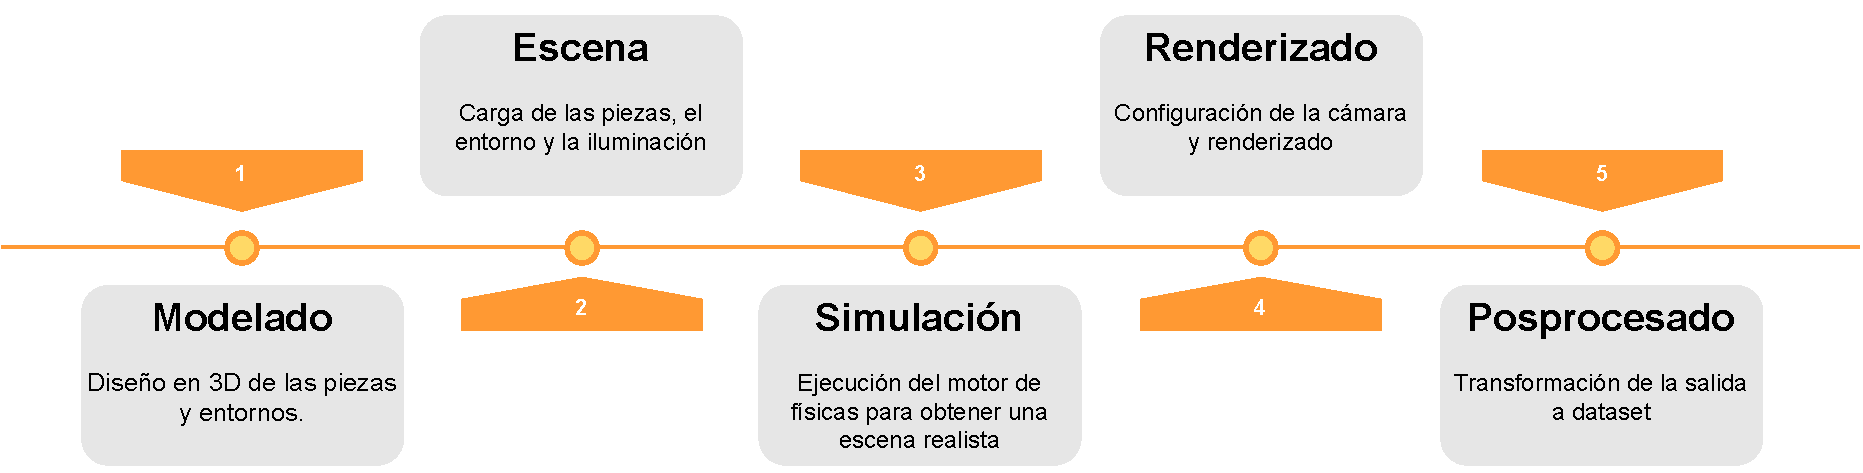
\includegraphics[width=0.9\textwidth]{Dataset/Arquitectura generador.pdf}
	\caption{Esquema de la arquitectura del sistema}
	\label{chap:Generación de un dataset fig:Arquitectura generador}
	\vspace{-5pt}
\end{figure}

Como se puede observar en la \autoref{chap:Generación de un dataset fig:Arquitectura generador}, se trata de un proceso iterativo constituido por varias etapas que se ejecutan en serie para la generación de cada nueva imagen. A excepción de la primera etapa que consiste en la generación de los modelos 3D, esta etapa no forma parte del generador pero este depende de la existencia de un modelo 3D con el que poder trabajar.

En esta etapa se han diseñado múltiples piezas de diferentes tamaños con la ayuda de Blender así como múltiples entornos sobre los que más adelante se dispondrán las piezas. Para las piezas se parte de un archivos .stl que contienen la información dimensional de las piezas. Estos han sido cargados en Blender donde se ha modificado el número de triángulos para mejorar el rendimiento y la suavidad de las piezas. Y se ha generado las texturas necesarias para las piezas las cuales incluyen defectos y patrones que deben de variar para cada instancia de estas añadiendo así aleatoriedad. Los entornos se han desarrollado por completo en Blender y se caracterizan por ser sencillos y planos. Su objetivo es contener a las piezas y no formar 0 confundirse con estas. Para los entornos se empleará una textura aleatoria para cada imagen de una librearía \textit{open source} CCTextures y constituida por más de mil seiscientas texturas de alta calidad.

Las piezas grandes requieren del uso de códigos QR que permitan en la etapa de posprocesado (\ref{chap:Generación de un dataset sec:Posprocesado}) extraer la información necesaria. Es por ello que en la etapa de modelado se debe de crear duplicados de las piezas grandes a los que se les insertará códigos QR en las zonas con posibles puntos de agarre.

Partiendo de los modelos y texturas necesarios, el sistema desarrollado puede empezar a generar imágenes:

\begin{enumerate}
\item Escena: Carga del entorno, de las piezas, la iluminación y la cámara
\begin{itemize}
\item Entorno: Se escoge de forma aleatoria uno de los entornos disponibles y se carga dentro de blender. A continuación, se escoge una de las texturas disponibles y se aplica en la totalidad del entorno. Por último, se centra el entorno y se deshabilita el cuerpo dentro del motor de físicas. De esta forma se fija la posición del entorno y este pasa a ser inalterable.

\item Piezas: Se escoge de forma aleatoria el número de piezas que estarán presentes en la escena (se establecen mínimos y máximos dependiendo del tamaño de la pieza) y se cargan dentro de blender. Por último, se define una propiedad \textit{category\_id} que más adelante será usada para identificar las distintas piezas.

\item Iluminación: Se parte de la base de que el entorno de trabajo real estará bien iluminado, por ello que se han definido unas condiciones de iluminación fijas y óptimas que permitan reducir las sombras. Se planteo emplear una iluminación aleatoria pero esta daba lugar a demasiadas sombras y dificultaba ver el contorno de las piezas oscuras.

\item Cámara: Para asemejarse a la realidad se ha fijado una cámara cenital a la escena y se ha implementado las parámetros intrínsecos de la cámara real que se va a emplear dentro de blender.
\end{itemize}

\item Simulación: activación de las piezas, posicionamiento de las piezas y simulación física.
\begin{itemize}
\item Activación de las piezas: se activa el motor de físicas para todas las piezas de forma que se vea afectadas por la gravedad y el entorno.
\item Posicionamiento de las piezas: con la ayuda de la \acs{api} de BlenderProc se posicionan todas las piezas de forma aleatoria dentro de un volumen de trabajo. El volumen de trabajo se fija en base a las dimensiones del entorno y la posición y orientación de la pieza se determina de forma aleatoria con el motor de aleatoriedad de numpy y BlenderProc.
\item Simulación física: se ejecuta una simulación física en la que se deja caer las piezas sobre el entorno/zona de trabajo. Se ejecuta el motor hasta que todas las piezas se vuelvan estáticas o se alcance el máximo tiempo de simulación de cuatro segundos.
\end{itemize}

\item Renderizado: configuración del motor de renderizado, renderizado y escritura de la salida de blender.
\begin{itemize}
\item Configuración: dependiendo del tamaño de la pieza se fija la configuración necesaria.
\begin{itemize}
\item Piezas grandes: resolución 3840x2160, 50 muestras y se activa el mapa de normales y de profundidad.
\item Piezas pequeñas: resolución 1920x1080, 25 muestras.
\end{itemize}
\item Renderizado: se activa el proceso o procesos de renderizado dependiendo del tamaño de la pieza.
\item Salida: se transfiere el resultado de los renderizados del archivo temporal de trabajo de blender al lugar de salida deseado.
\end{itemize}
\end{enumerate}

\begin{figure}[ht]
\centering
\begin{tabular}{cccc}
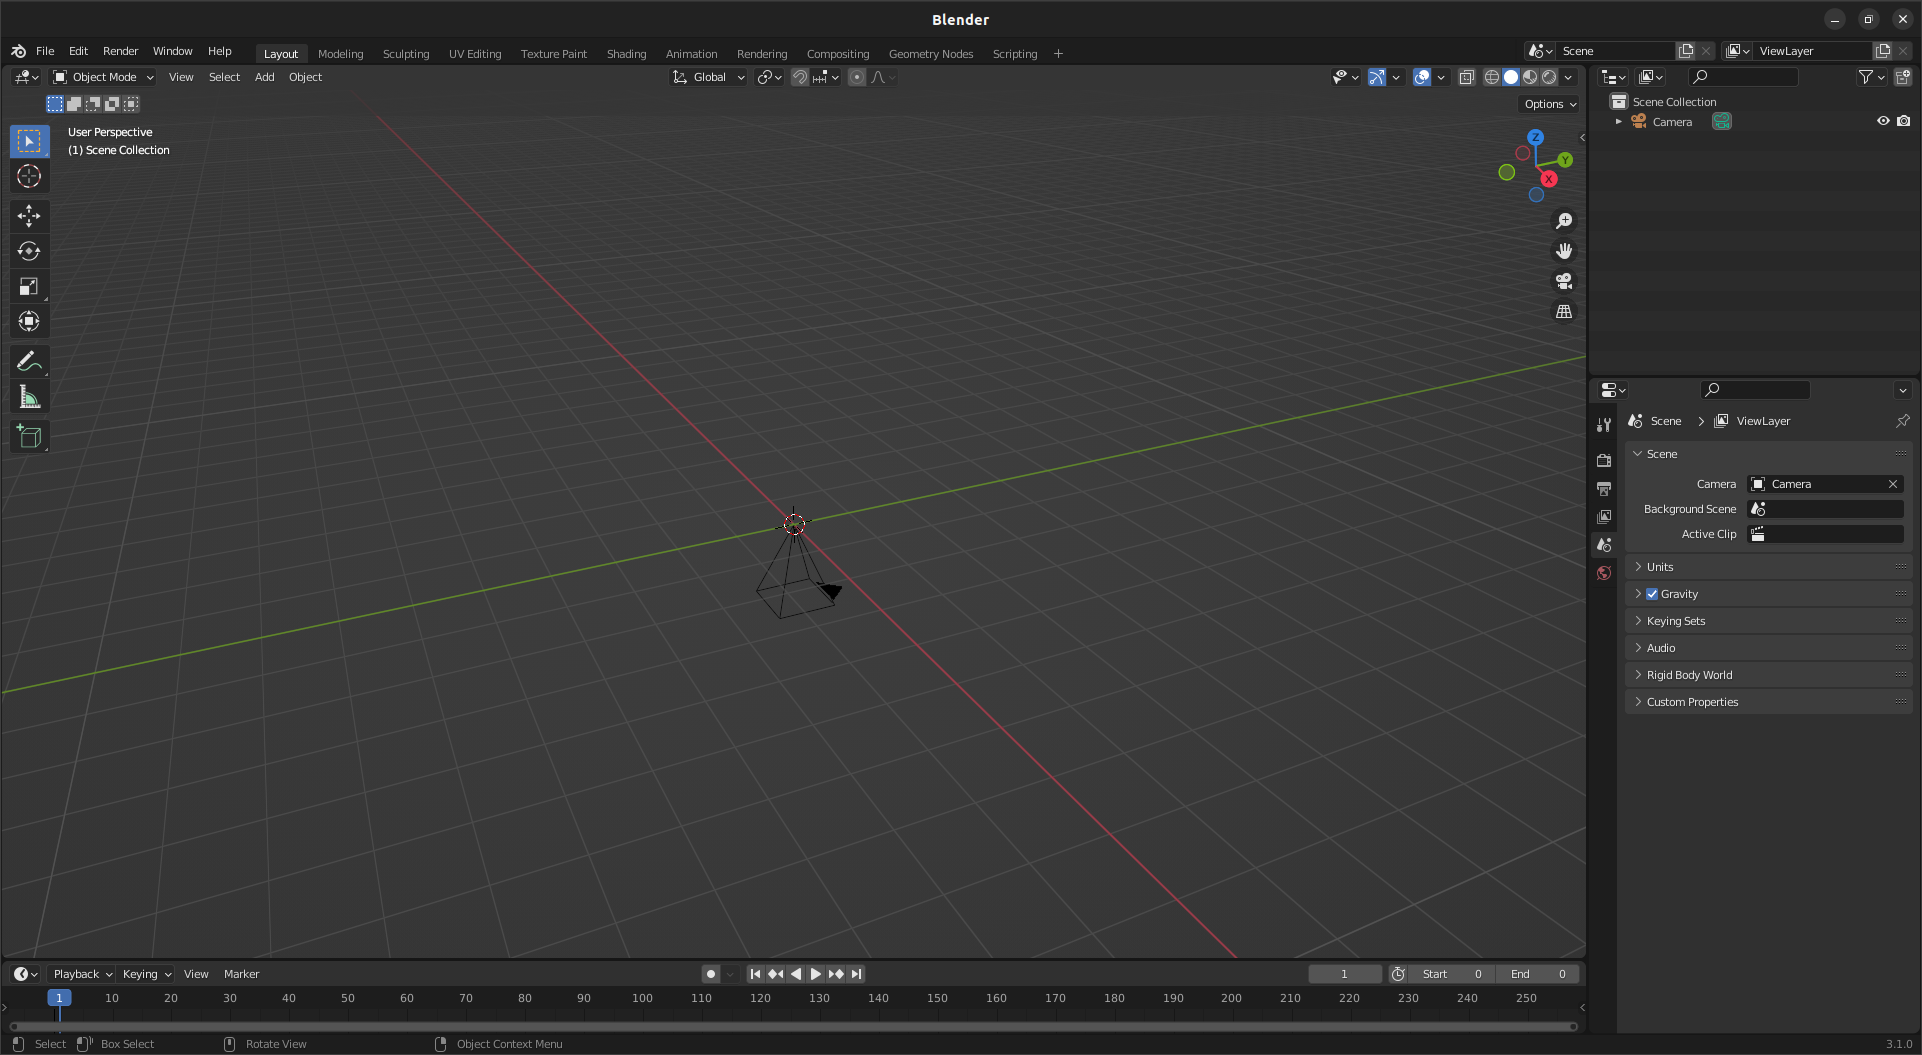
\includegraphics[width=0.3\textwidth]{Dataset/blender_normal_1.png} &
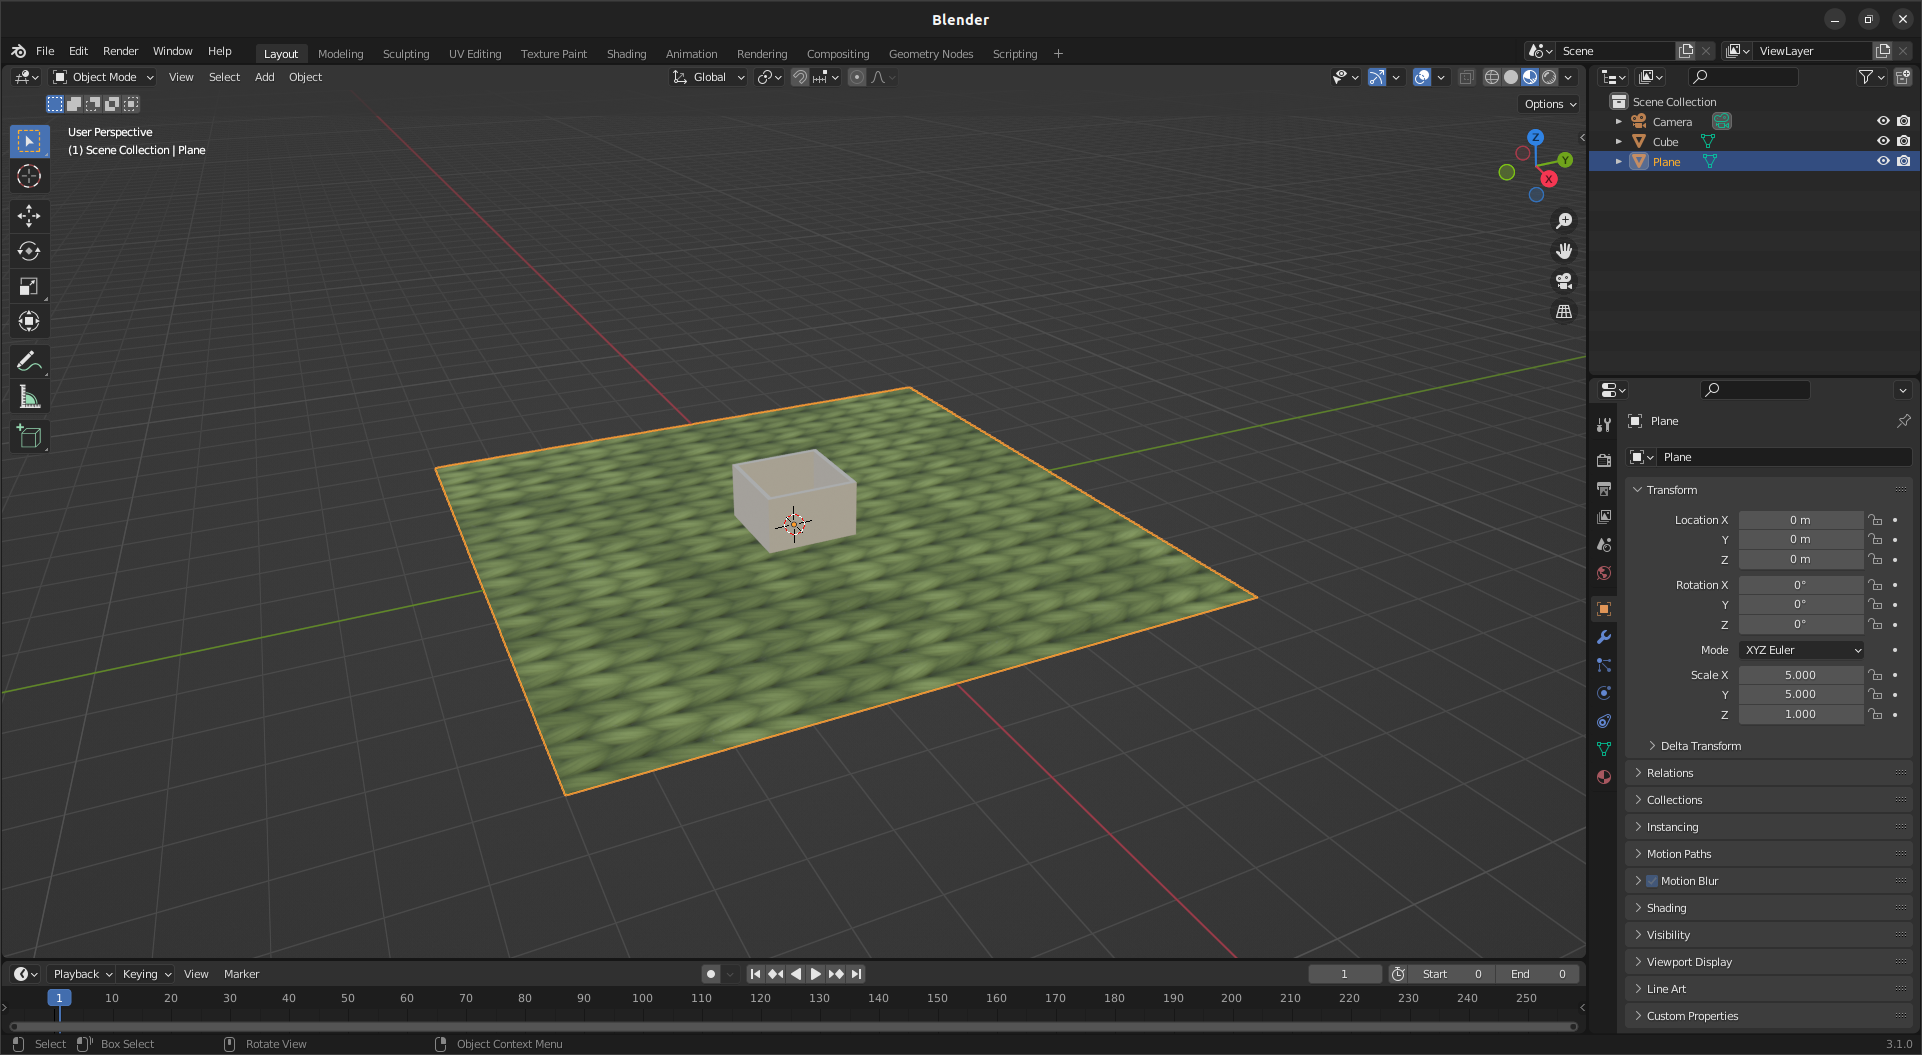
\includegraphics[width=0.3\textwidth]{Dataset/blender_normal_2.png} &
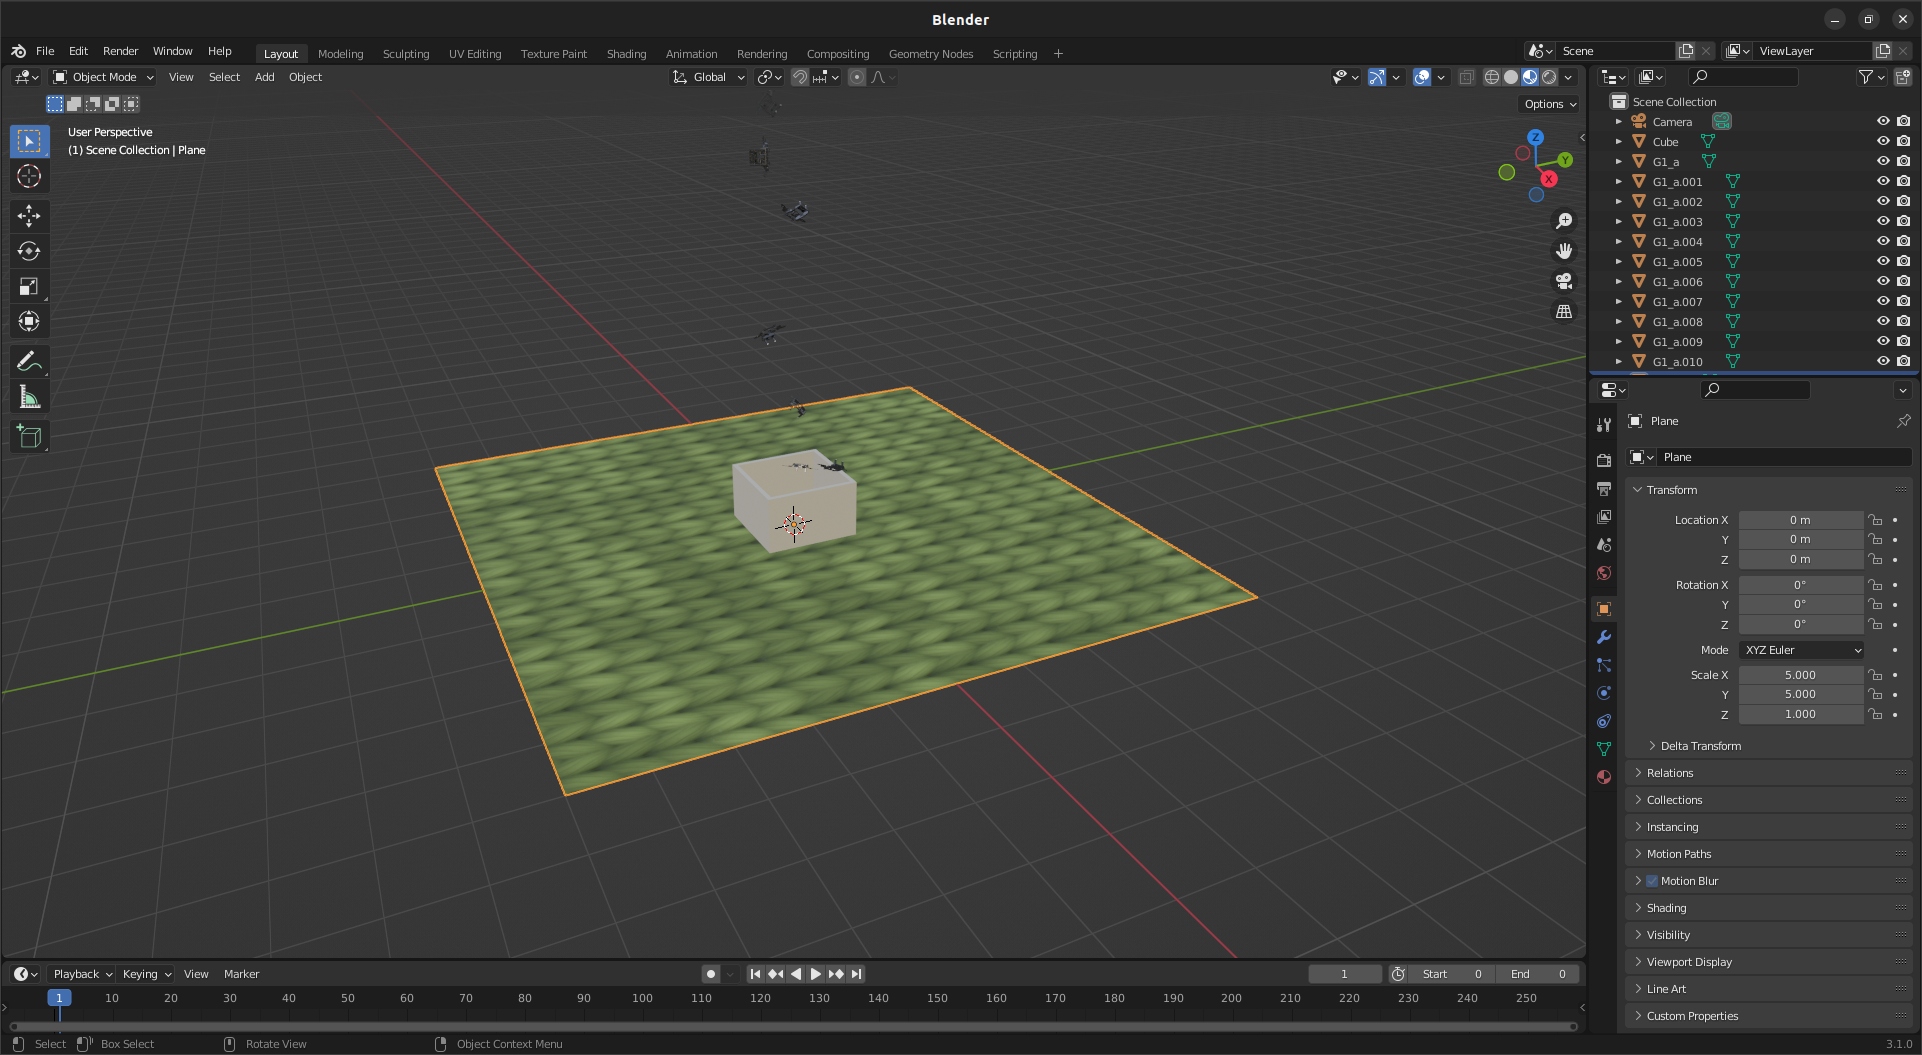
\includegraphics[width=0.3\textwidth]{Dataset/blender_normal_3.png} \\
Inicio  & Carga del escenario & Carga de piezas  \\[6pt]
\end{tabular}
\begin{tabular}{cccc}
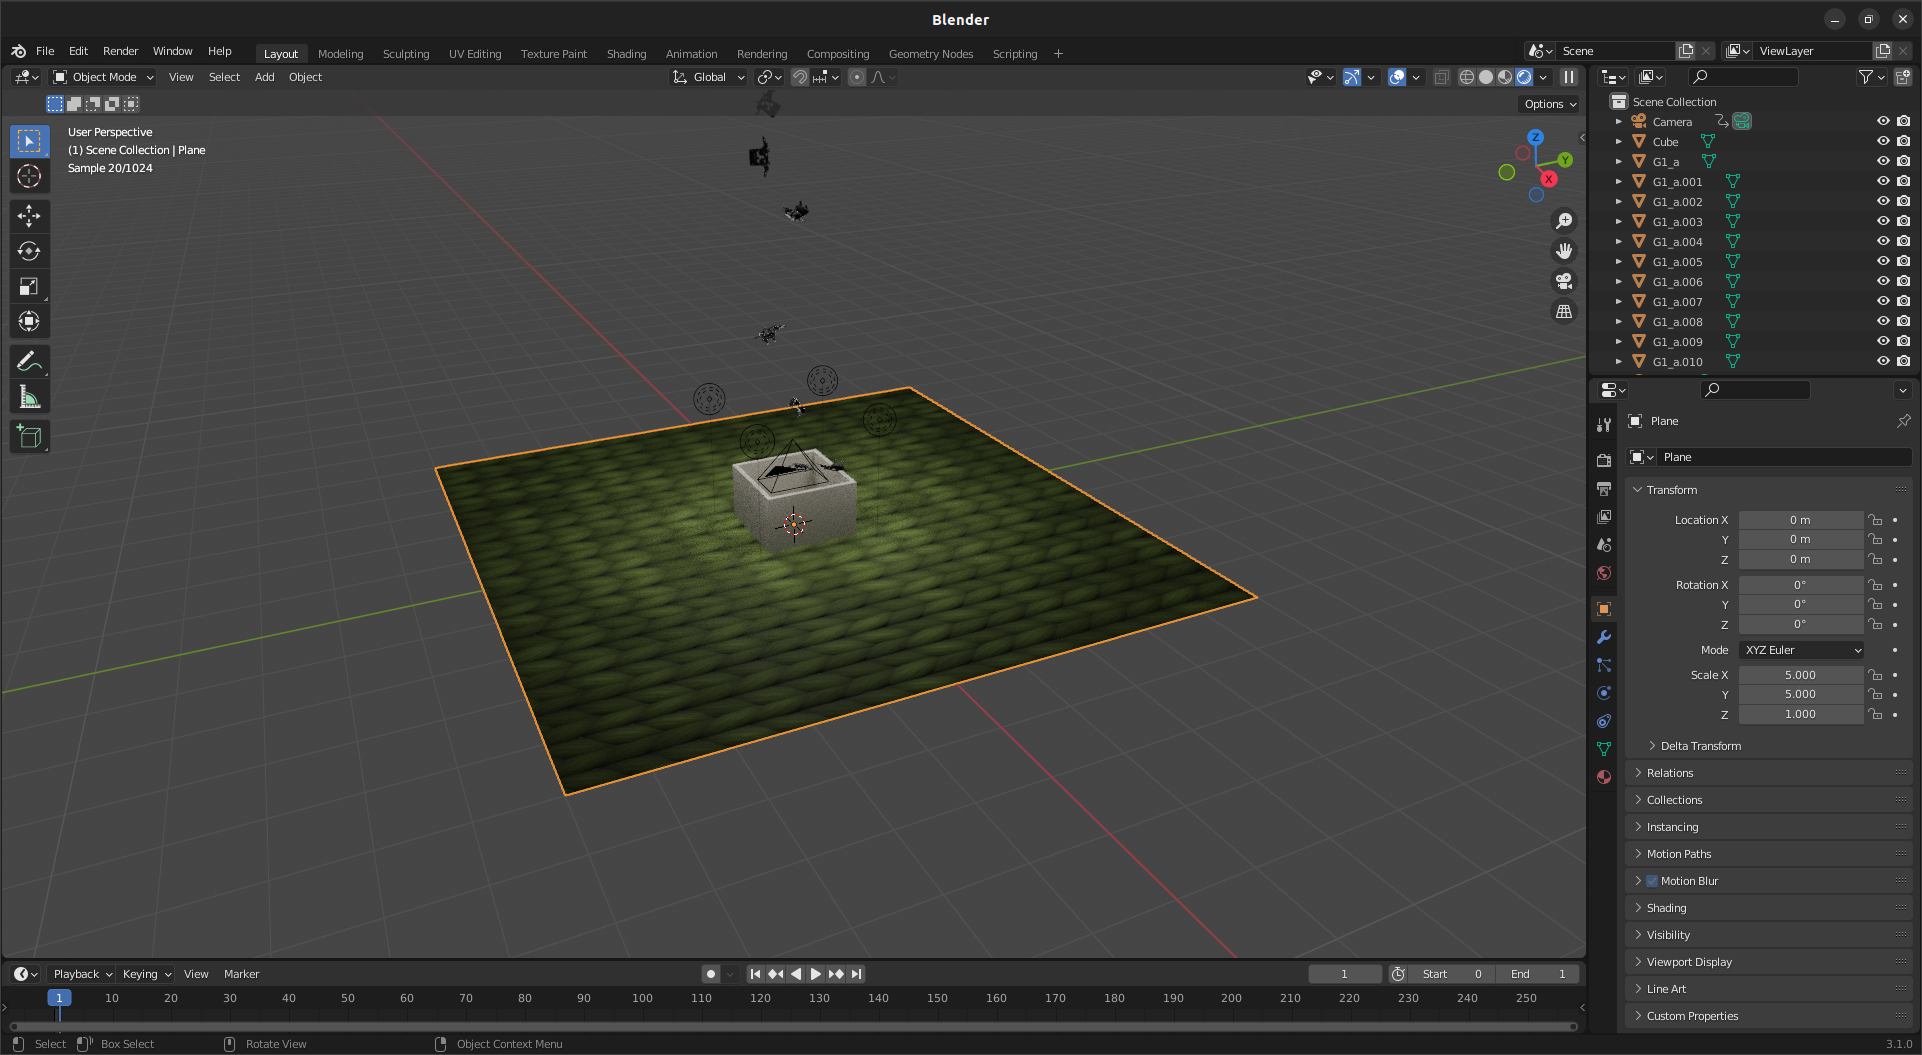
\includegraphics[width=0.3\textwidth]{Dataset/blender_normal_4.png} &
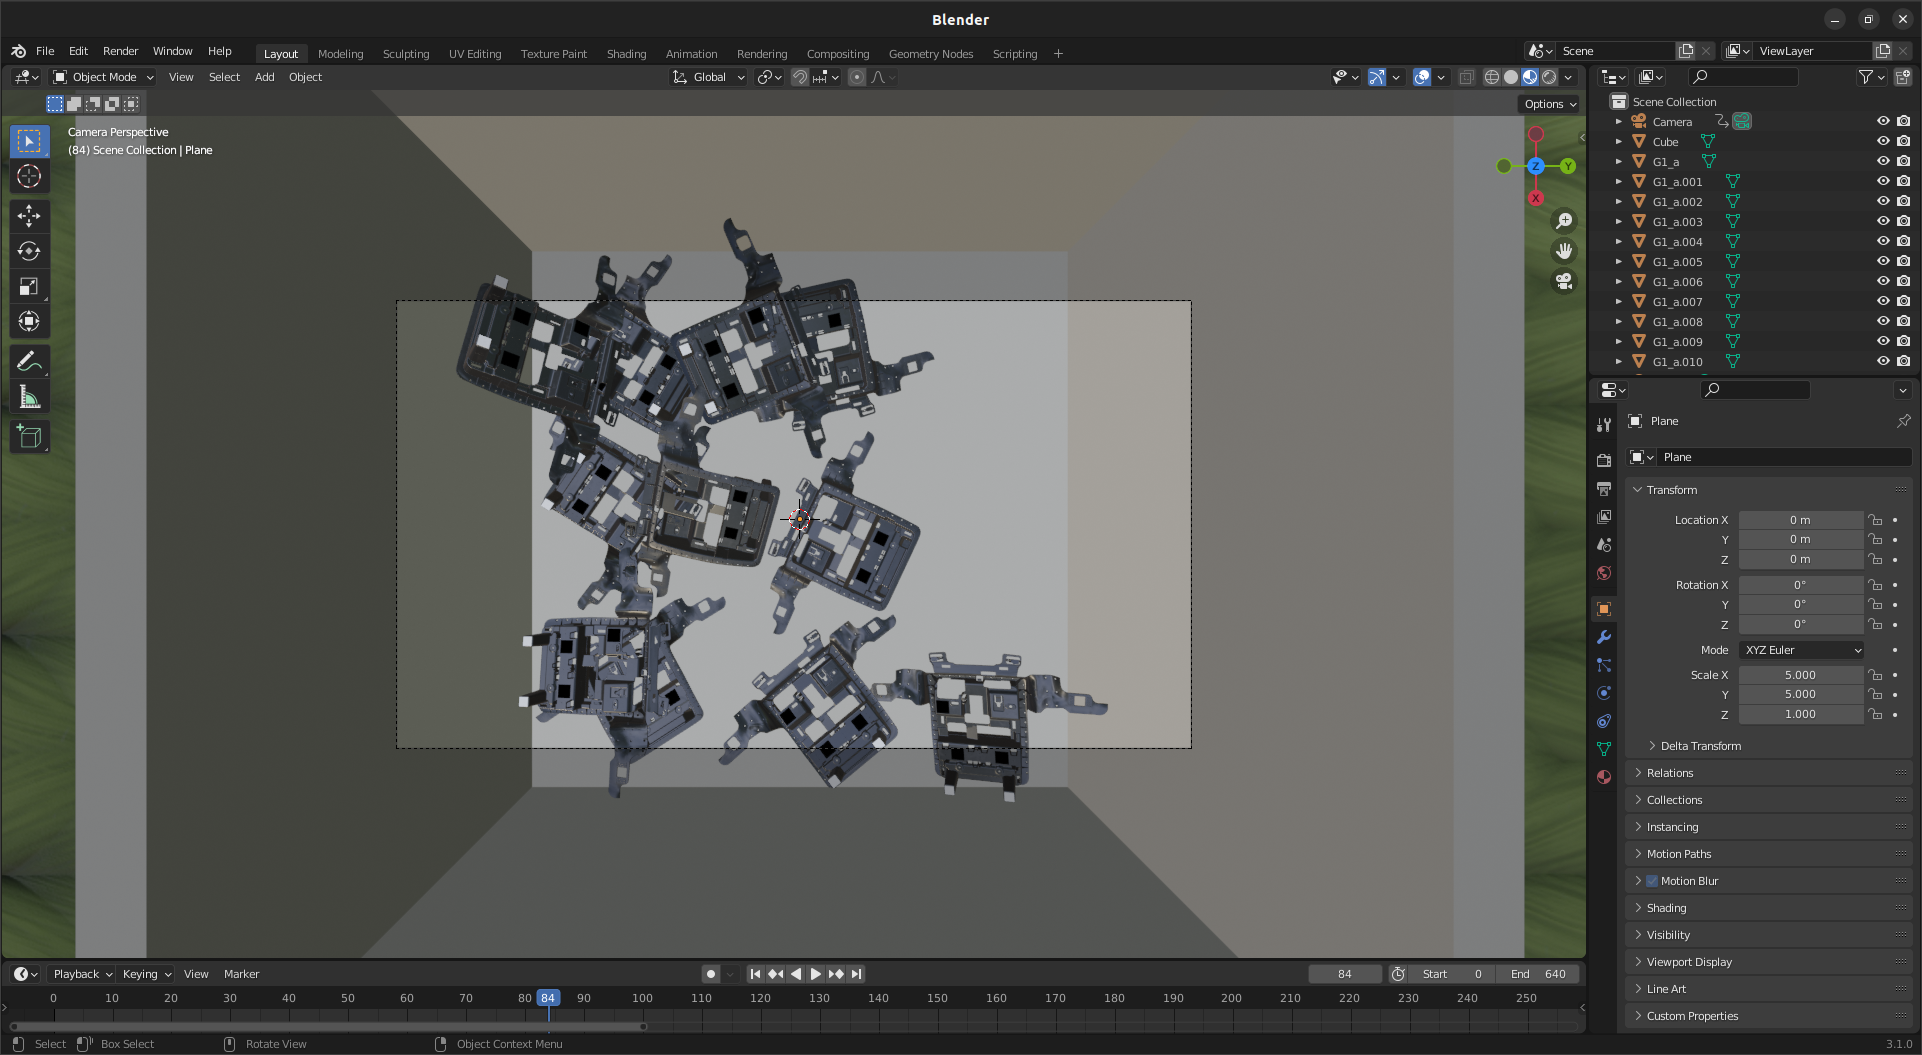
\includegraphics[width=0.3\textwidth]{Dataset/blender_normal_5.png} &
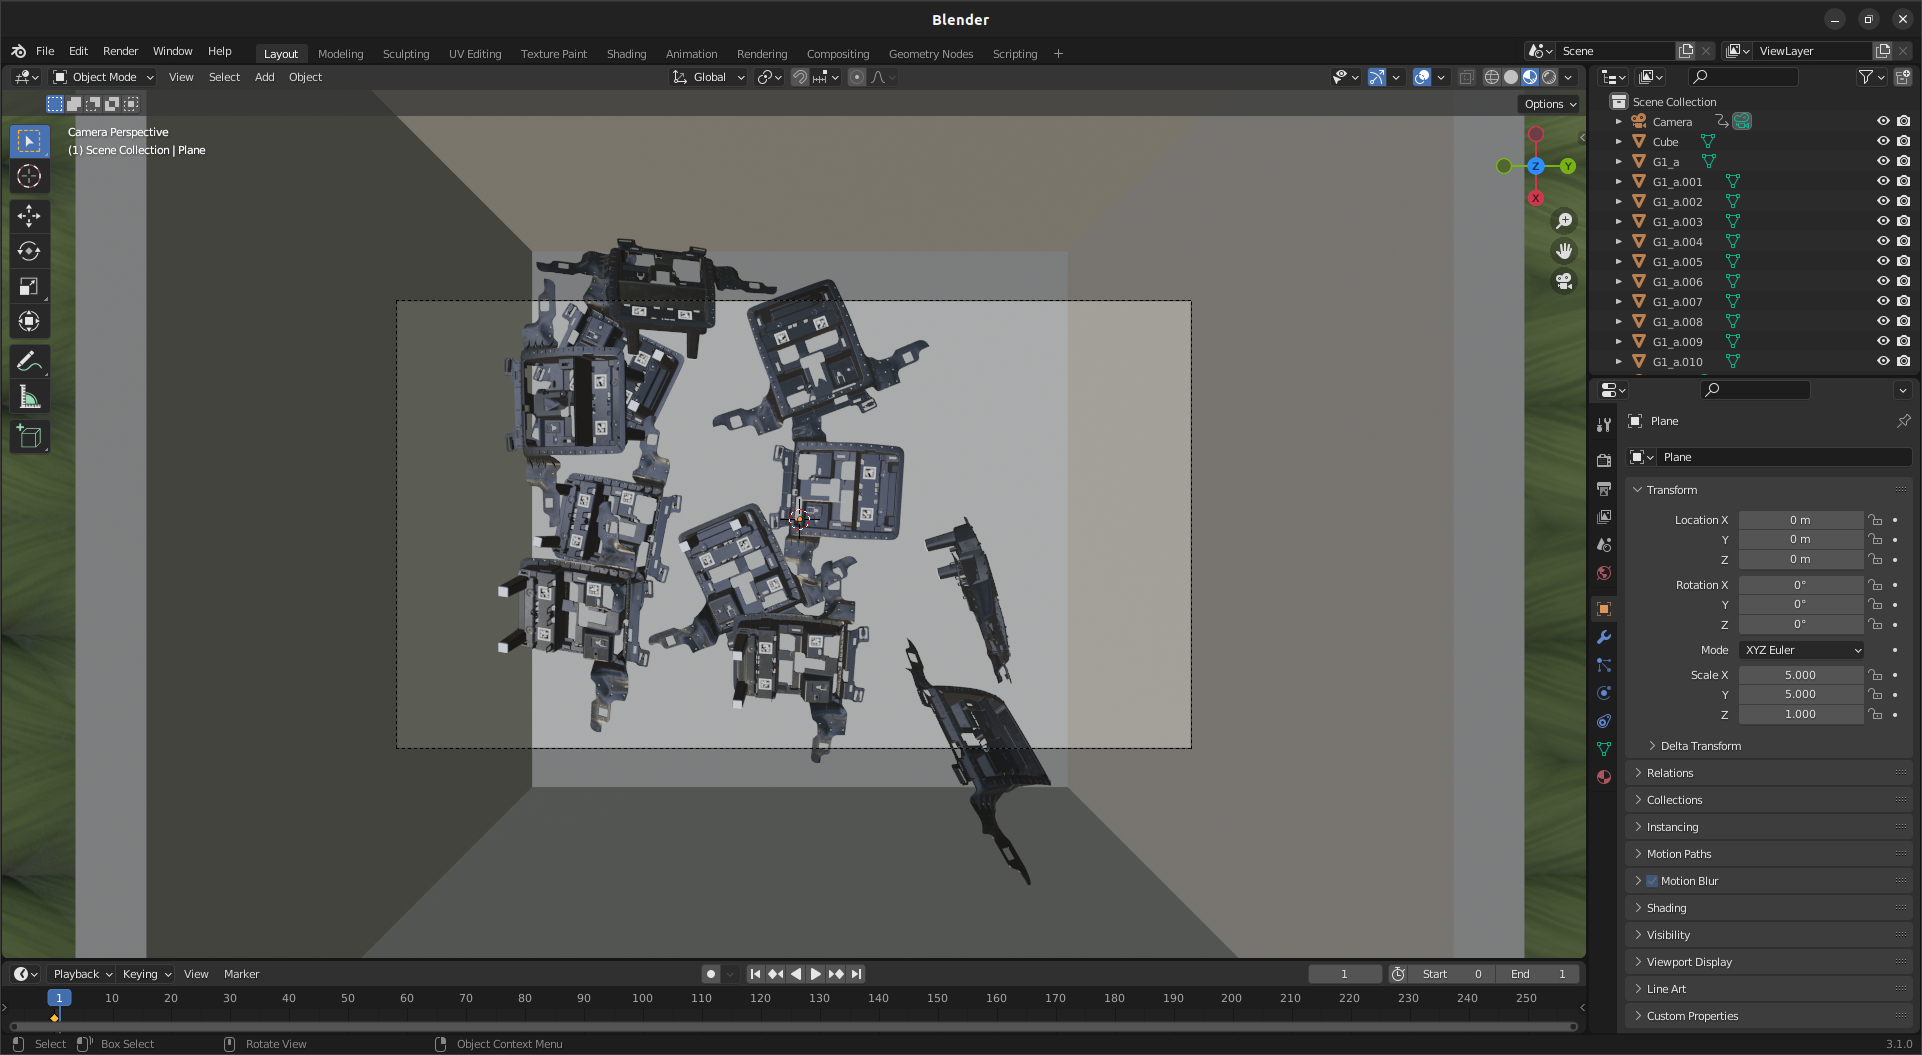
\includegraphics[width=0.3\textwidth]{Dataset/blender_aruco_1.png} \\
Iluminación y cámara  & Configuración normal & Configuración aruco  \\[6pt]
\end{tabular}
\begin{tabular}{cccc}
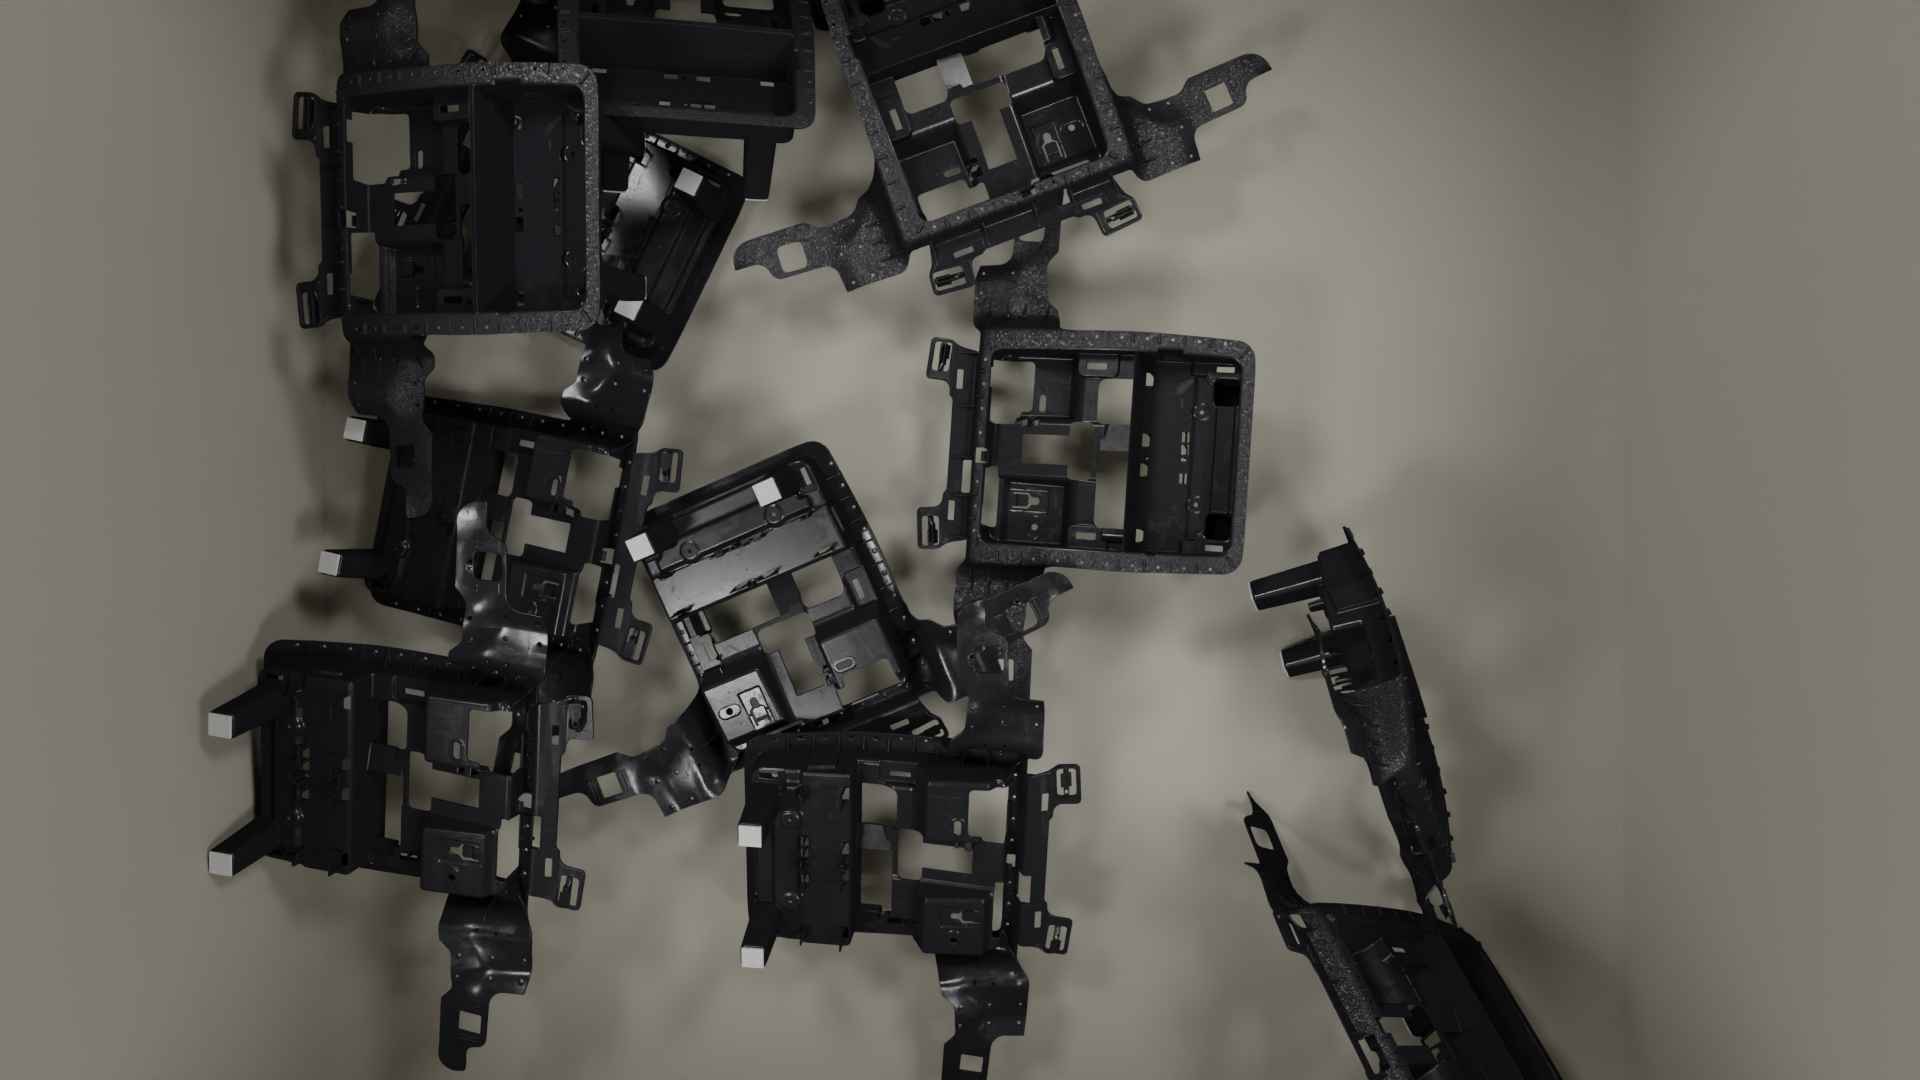
\includegraphics[width=0.3\textwidth]{Dataset/blender_normal_6.png} &
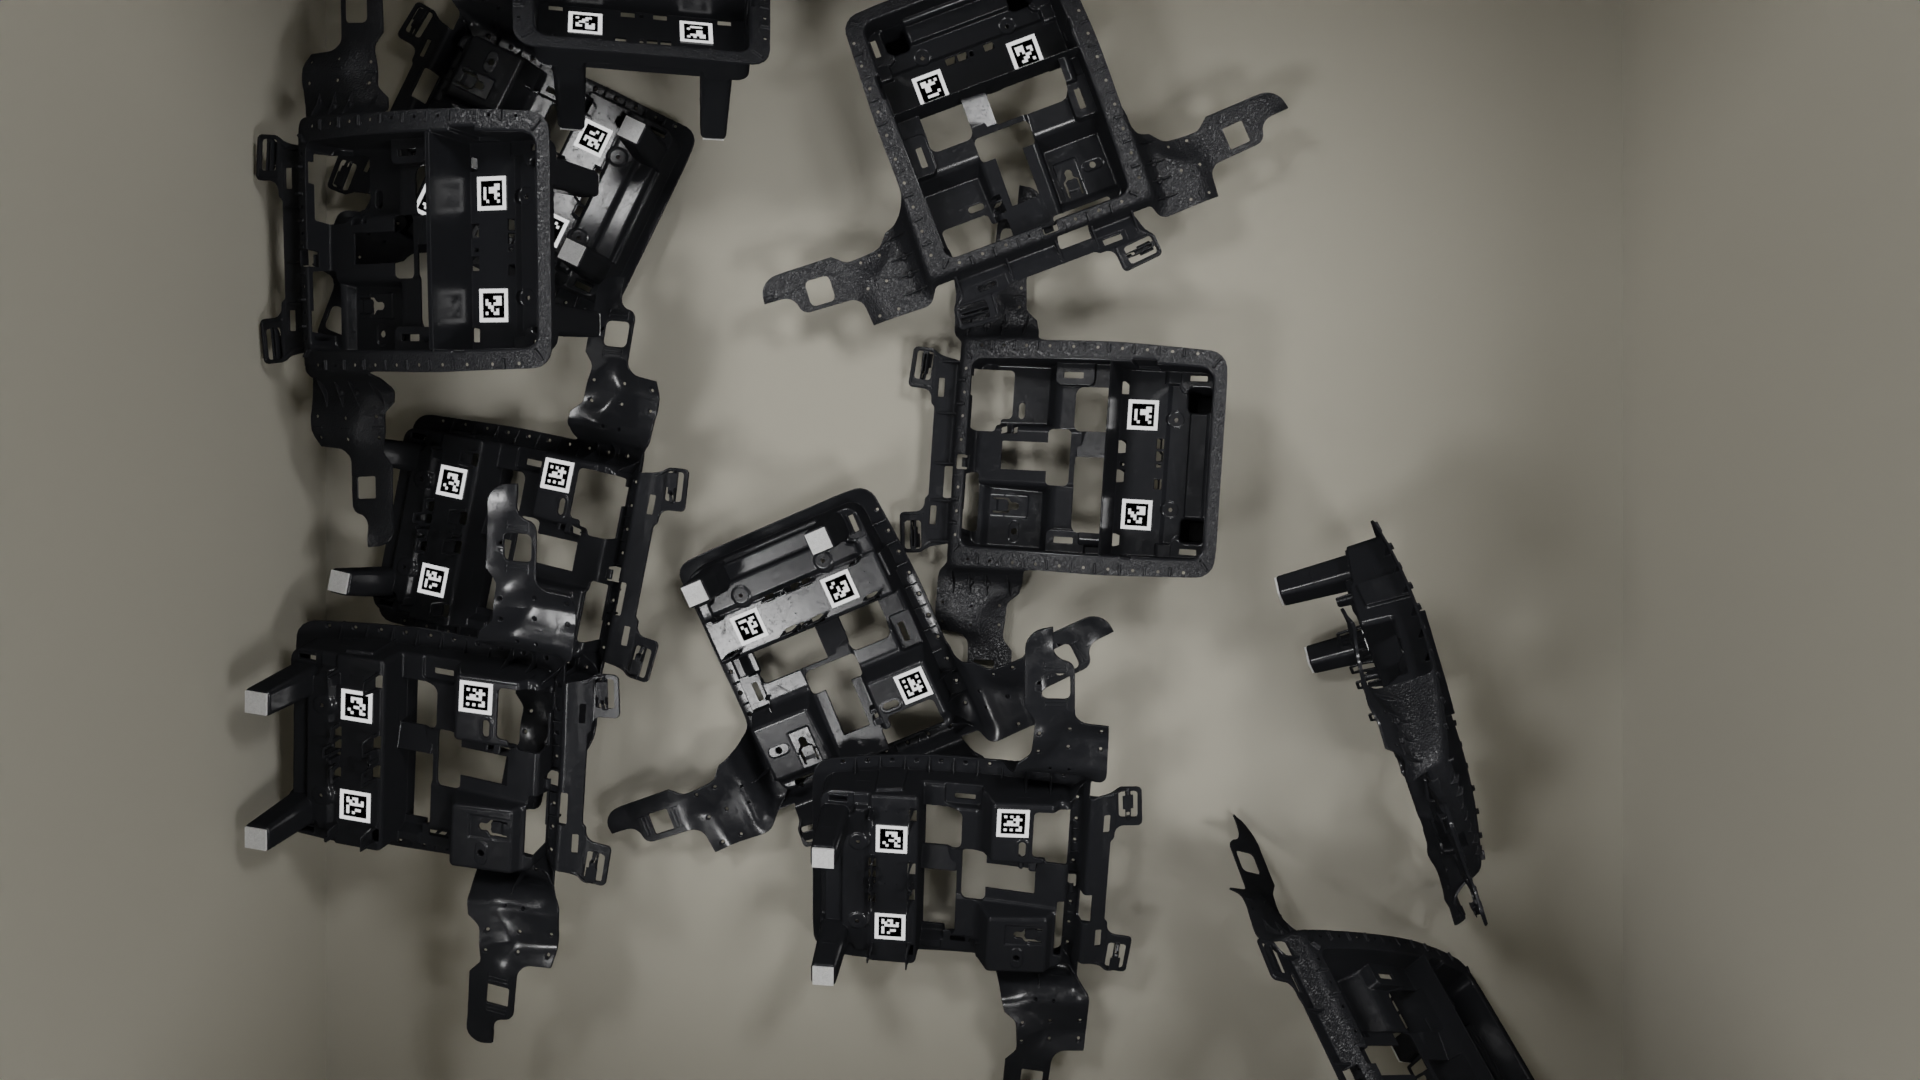
\includegraphics[width=0.3\textwidth]{Dataset/blender_aruco_2.png} \\
Render normal  & Render Aruco  \\[6pt]
\end{tabular}
\caption{Proceso de generación de imágenes}
\label{chap:Generación de un dataset fig:Proceso de generación}
\end{figure}


\section{Posprocesado}
\label{chap:Generación de un dataset sec:Posprocesado}
El \textit{dataset} deseado debe de contener para cada imagen una lista de todas las piezas presentes asi como su posición y los puntos de agarres disponibles. Esta información no se puede obtener de forma directo con Blender y BlenderProc, es por ello que se ha tenido que desarrollar varios sistemas de posprocesado específicos para cada uno de los componentes de la red neuronal.

\begin{itemize}
\item Posición (\textit{YOLO}): el primer procesado se caracteriza por ser una simple transformación de la información generada por Blender y BlenderProc a un formato que la red neuronal pueda entender. El generador de imágenes es capaz de crear un archivo de texto conteniendo la posición de las piezas en la imagen y el mapa de segmentación. Sin embargo, estas se encuentran en un formato distinto al empleado por la red neuronal. La transformación empleada consiste en un cambio de origen de la posición de las piezas y en la eliminación del resto de información que no es relevante. El proceso a seguir se muestra a continuación:
\vspace{5 mm}
\lstinputlisting[language=Python]{codigo/Prepare_Dataset_YOLO.py}
\vspace{5 mm}

\item Zonas de interés (\textit{Tiny YOLO}): el segundo procesado debe de determinar para cada piezas las posibles zonas de agarre. Para ello se debe de obtener para cada imagen un recorte de cada pieza presente en la imagen. Y la posición de las zonas de interés de cada recorte. Para llevar a cabo esta tarea se va a emplear la librearía Aruco que se caracteriza por poder detectar códigos QR con precisión, rapidez y eficiencia. El proceso a seguir se muestra a continuación:
\vspace{5 mm}
\lstinputlisting[language=Python]{codigo/Prepare_Dataset_TINY_YOLO.py}
\vspace{5 mm}

\item Vectores normales (Regresor): el objetivo es obtener los vectores normales y el punto de agarre para cada pieza. Por ello la salida en este caso será una imagen individual para cada pieza y un archivo de texto para cada punto de la pieza. En este archivo se almacenarán los centros de cada punto y las coordenadas de su vector normal. El proceso para la obtención de la imagen de cada pieza individual es idéntico al de las zonas de interés. Este posprocesado se caracteriza por el tratamiento de la imagen de normales y la generación de los archivos de texto con la información de cada punto de agarre. El proceso a seguir se muestra a continuación:
\vspace{5 mm}
\lstinputlisting[language=Python]{codigo/Prepare_Dataset_Regressor.py}
\vspace{5 mm}

\end{itemize}


\section{Aleatoriedad}
\label{chap:Generación de un dataset sec:Aleatoriedad}
Uno de los factores más importantes durante el desarrollo de este sistema es el sesgado. Se debe de evitar que el sistema genere un \textit{dataset} sesgado lo cual implica comprobar y asegurar la aleatoriedad de los resultados obtenidos. Para ello se empleará siempre que sea posible motores de aleatoriedad. Estos se caracterizan por ser capaces de obtener distribuciones uniformes (la mayor expresión de la aleatoriedad ya que todos los resultados son equitativamente probables). Con la excepción del generador de rotaciones aleatorias, ya que debido a la naturaleza de los ángulos de euler la distribución no puede ser uniforme. Durante el proceso de generación de imágenes se emplea un total de tres motores de aleatoriedad. Para asegurar la veracidad de estos tres motores, se ha realizado una serie de pruebas con diferentes semillas y múltiples muestras. A continuación, se muestras los resultados de todos los motores de aleatoriedad empleados.

El primer motor empleado se trata del generador de una distribución uniforme de numpy. Como su nombre indica, se encarga de generar un valor entre los máximos y mínimos establecidos de forma que todos los valores presenten la misma probabilidad. Este método es empleado para determinar el número de piezas que se deben de cargar así como su posición dentro de la zona de trabajo.

El segundo motor empleado es \textit{choice} del paquete \textit{random} de Python. Este se encarga de escoger de forma aleatoria un elemento de una lista. Se debe de asegurar de que todos los elementos presenten la misma probabilidad de ser escogidos. Este método es empleado para determinar que tipo de escenas, piezas y texturas se deben de emplear.

El último motor empleado es \textit{UniformSO3} de BlenderProc. Este se encarga de determinar una rotación aleatoria para las piezas. Esta rotación esta definida por ángulos de euler, es por ello que las distribuciones no deben de ser uniformes. Esto se debe a que una misma posición puede ser alcanzada por diferentes combinaciones de ángulos.

\begin{figure}[ht]
	\ContinuedFloat
	\centering
	\begin{subfigure}[b]{0.3\linewidth}
		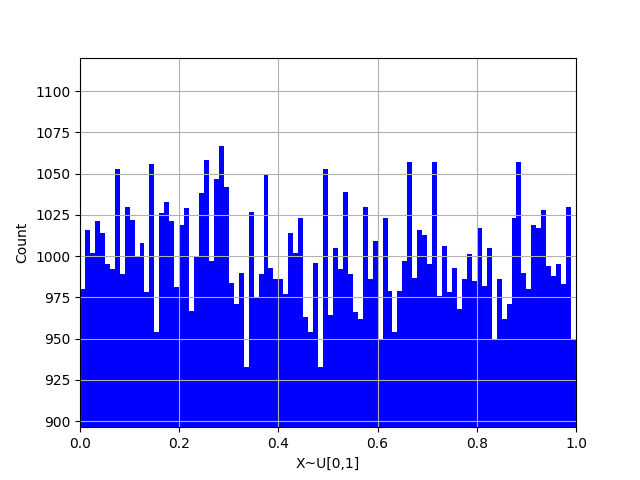
\includegraphics[width=\linewidth]{Dataset/numpy_uniform_histogram_10.png}
	\end{subfigure}
	\begin{subfigure}[b]{0.3\linewidth}
		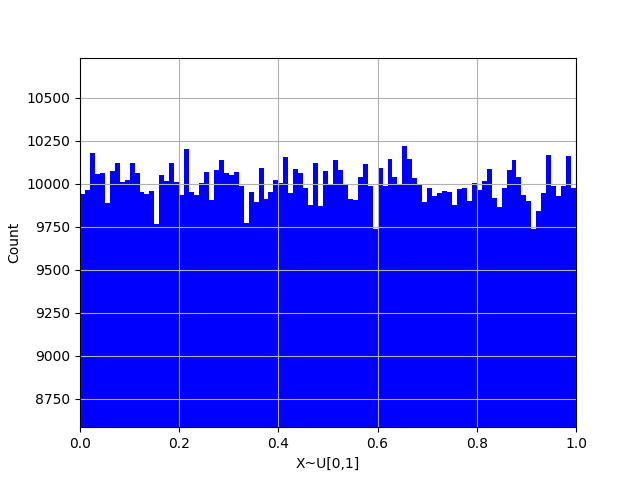
\includegraphics[width=\linewidth]{Dataset/numpy_uniform_histogram_100.png}
	\end{subfigure}
	\begin{subfigure}[b]{0.3\linewidth}
		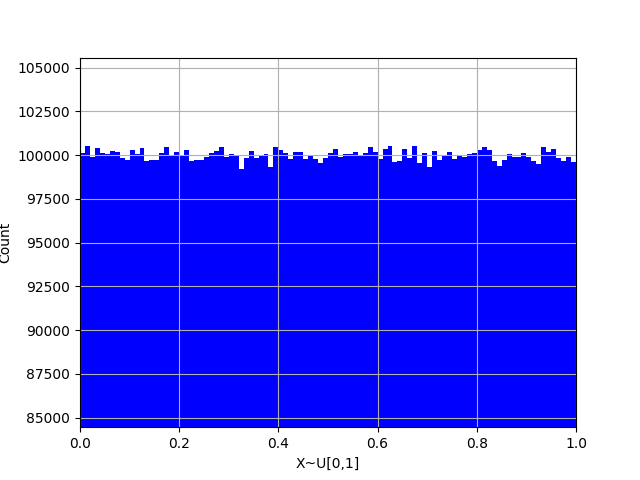
\includegraphics[width=\linewidth]{Dataset/numpy_uniform_histogram_1000.png}
	\end{subfigure}
	\caption{Aleatoriedad de una distribución uniforma generada por numpy}
	\label{chap:Generación de un dataset fig:numpy uniform}
	
	\begin{subfigure}[b]{0.3\linewidth}
		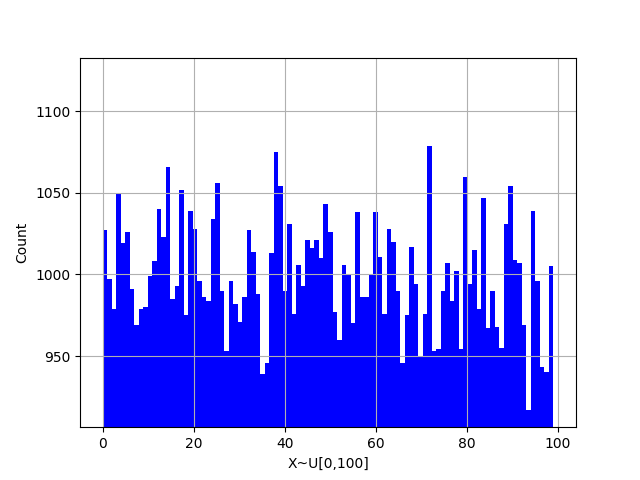
\includegraphics[width=\linewidth]{Dataset/random_choice_histogram_10.png}
	\end{subfigure}
	\begin{subfigure}[b]{0.3\linewidth}
		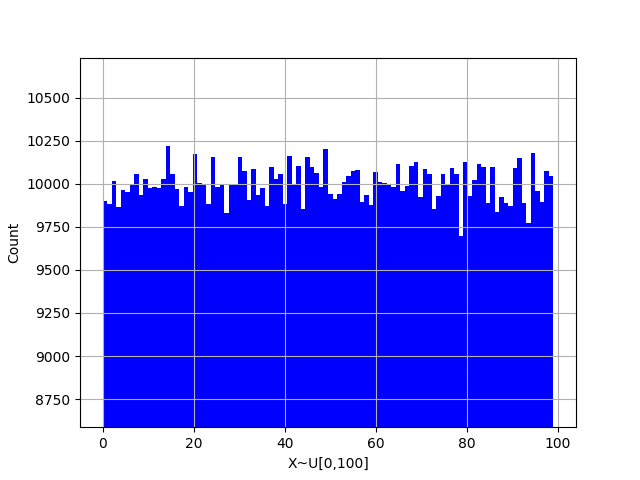
\includegraphics[width=\linewidth]{Dataset/random_choice_histogram_100.png}
	\end{subfigure}
	\begin{subfigure}[b]{0.3\linewidth}
		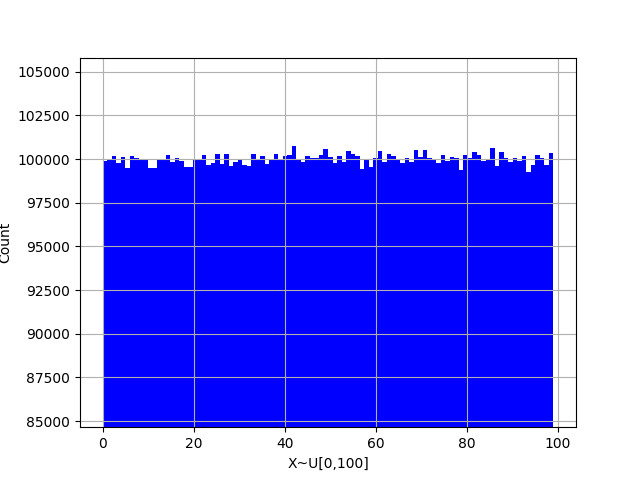
\includegraphics[width=\linewidth]{Dataset/random_choice_histogram_1000.png}
	\end{subfigure}
	\caption{Aleatoriedad del comando \textit{choice} del paquete \textit{random}}
	\label{chap:Generación de un dataset fig:random choice}
	
	\begin{subfigure}[b]{0.3\linewidth}
		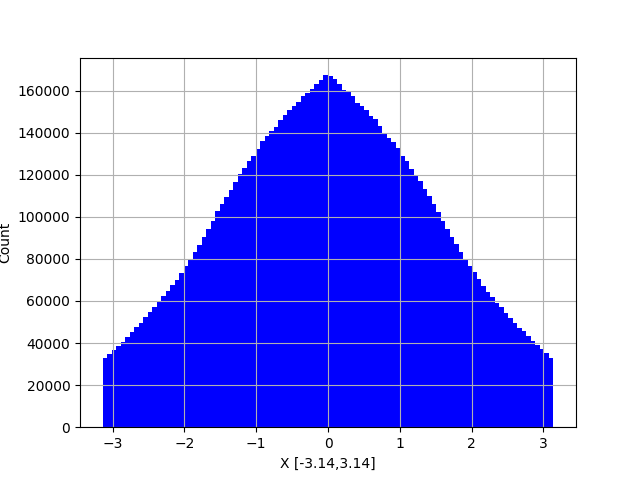
\includegraphics[width=\linewidth]{Dataset/blenderproc_uniformS03_histogram_1.png}
	\end{subfigure}
	\begin{subfigure}[b]{0.3\linewidth}
		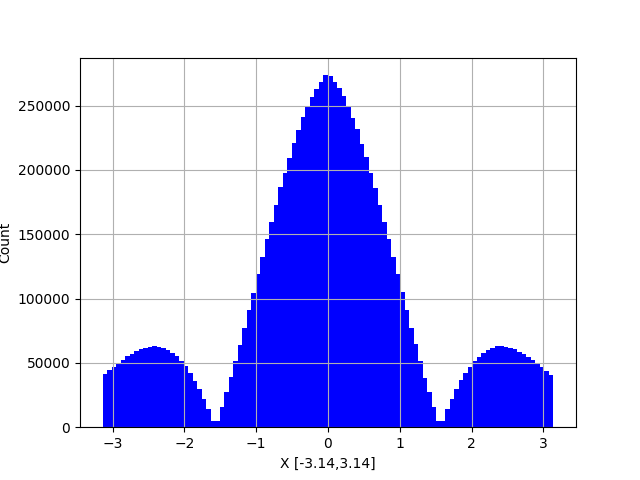
\includegraphics[width=\linewidth]{Dataset/blenderproc_uniformS03_histogram_2.png}
	\end{subfigure}
	\begin{subfigure}[b]{0.3\linewidth}
		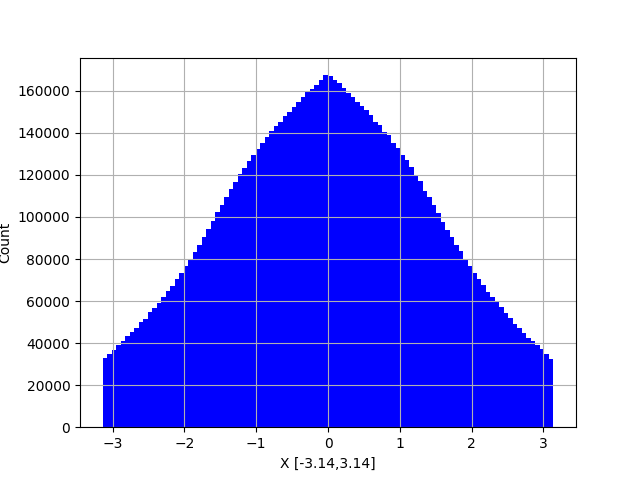
\includegraphics[width=\linewidth]{Dataset/blenderproc_uniformS03_histogram_3.png}
	\end{subfigure}
	\caption{Aleatoriedad de \textit{uniformSO3} del paquete BlenderProc}
	\label{chap:Generación de un dataset fig:uniformS03}
\end{figure}

\section{Resultados}
\label{chap:Generación de un dataset sec:Resultados}
Gracias a la implantación de un generador de imágenes se ha conseguido obtener un elevado número de instancias con las que poder entrenar la red neuronal que reflejan en gran medida la realidad. A continuación se muestran algunas de las imágenes obtenidas por es ambos sistemas.

\begin{figure}[ht]
	\ContinuedFloat
	\centering
	\begin{subfigure}[b]{0.3\linewidth}
		\includegraphics[width=\linewidth]{Dataset/Muestra_G1_a_sintetica.png}
	\end{subfigure}
	\begin{subfigure}[b]{0.3\linewidth}
		\includegraphics[width=\linewidth]{Dataset/Muestra_G3_sintetica.png}
	\end{subfigure}
	\begin{subfigure}[b]{0.3\linewidth}
		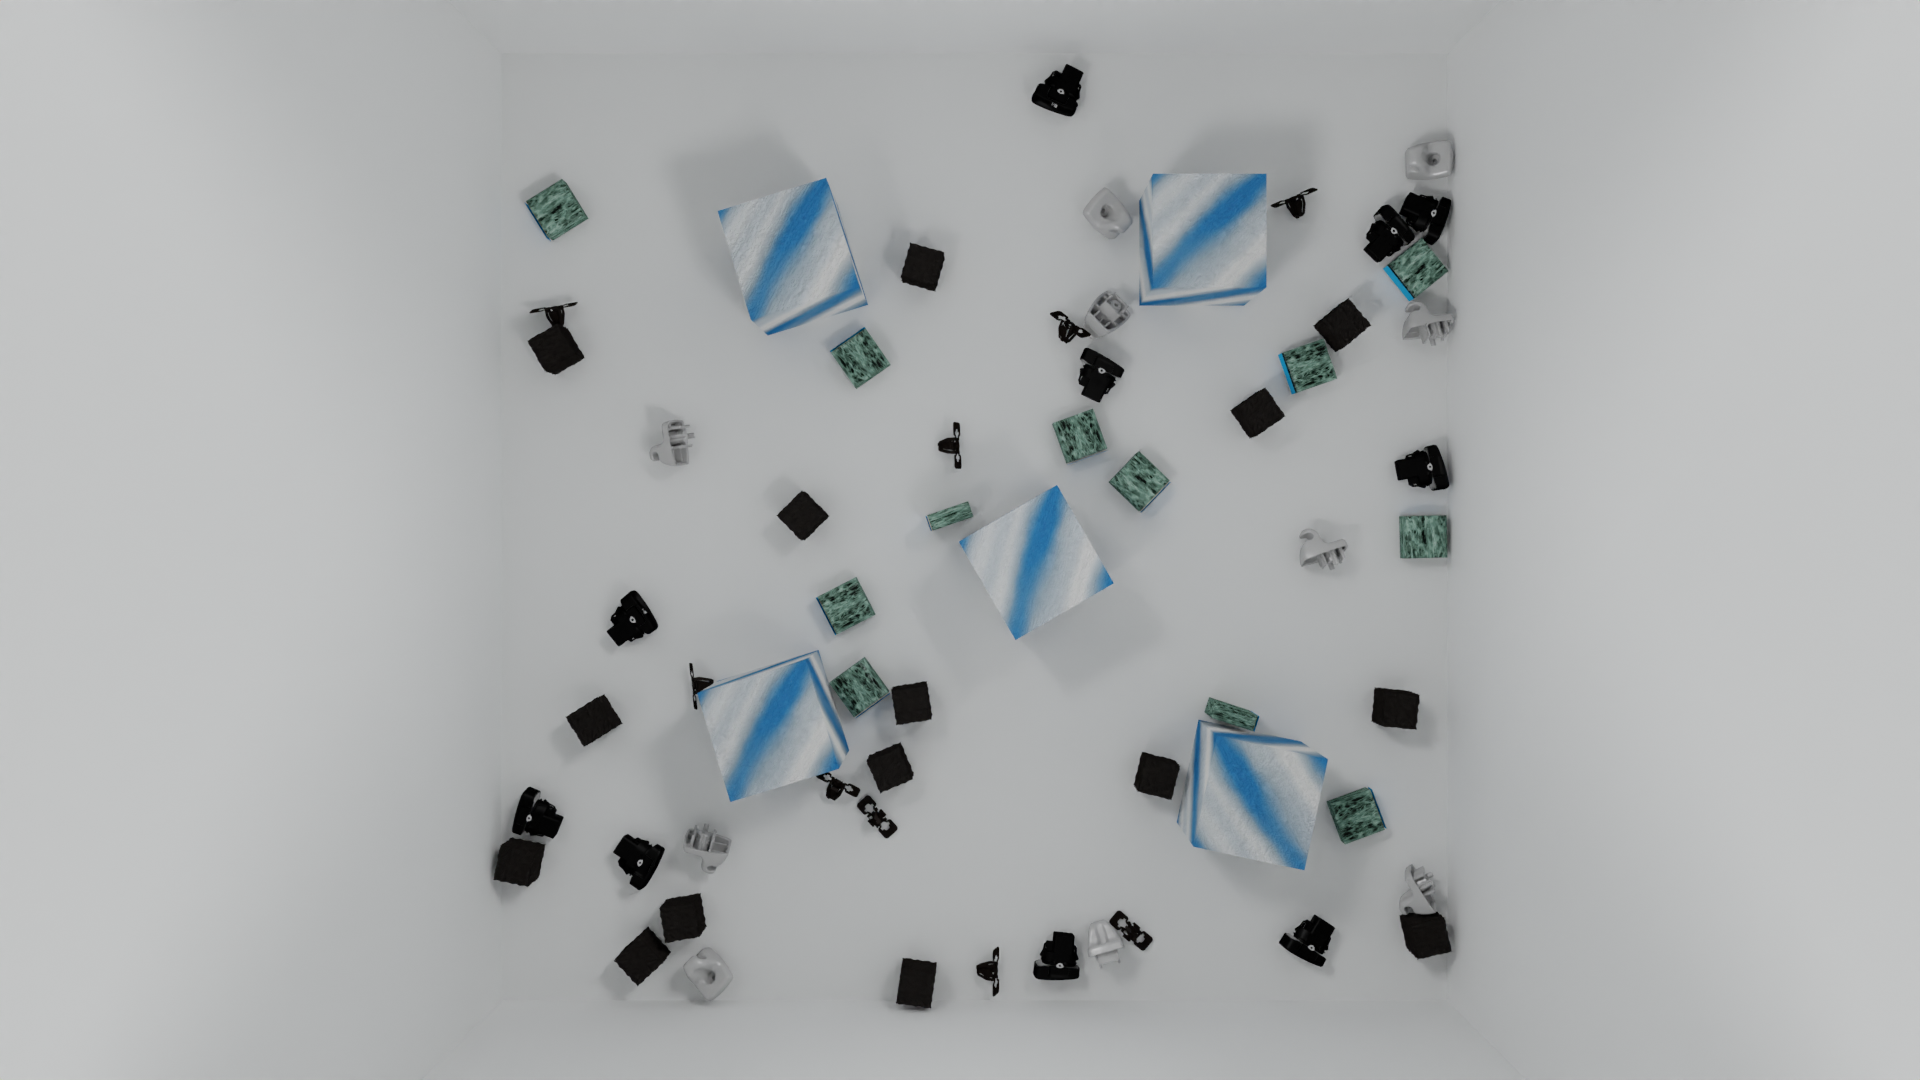
\includegraphics[width=\linewidth]{Dataset/Muestra_small_sintetica.png}
	\end{subfigure}
	\caption{Muestra de imágenes obtenidas mediante el generador de imágenes}
	\label{chap:Generación de un dataset fig:Muestras BlenderProc}

\end{figure}

Como se ha mencionado previamente, es importante entrenar modelos de redes neuronales con \textit{datasets} no sesgados. Esto implica que antes de entrenar un modelo se debe de analizar los datos para comprobar que se cumplen dichos requisitos. Para ello se han desarrollado una serie de \textit{scripts} en Python que permitirán mostrar el verdadero estado del \textit{dataset}.

Como para el desarrollo de este proyecto se deben de desarrollar tres modelos de redes neuronales, se debe de analizar los datos necesarios correspondiente a cada uno de estos modelos:

\begin{itemize}
\item \textit{YOLO}: se trata de la primera red neuronal empleada y desarrollada. Se encargará de detectar las piezas dentro de la zona de trabajo y se empleará como base para decidir que pieza se debe de recolectar. La salida de este modelo debe de ser las piezas presentes en la imagen y su posición. Por ello, para poder ser entrenada correctamente se debe de disponer de un número de instancias similares para cada pieza que se desea detectar.

\item \textit{Tiny YOLO}: una red neuronal menor y menos potente pero con una mayor especialización. Esta red se encargará de determinar regiones con posibles puntos de agarre dentro de las piezas (previamente identificadas por \textit{YOLO}). Esta segunda capa es especifica para cada pieza y solo se aplicará a aquellas piezas de elevado volumen. Es por ello que para el análisis de los datos de entrenamiento nos debemos de fijar de forma individual e independiente en cada pieza. En este caso nos vamos a centrar en las piezas G1 y G3 y en el número de instancias de cada zona de interés presente en estas.

\item Regresor: se trata de la última capa del sistema de visión artificial. Se basa en la salida del \textit{Tiny YOLO} y determina para cada una de las posibles regiones de interés el punto de agarre óptimo y su vector normal. Esta última capa es especifica para cada pieza y solo se aplicará a aquellas piezas de elevado volumen. Es por ello que para el análisis de los datos de entrenamiento nos debemos de fijar de forma individual e independiente en cada pieza. Además, al tratarse de un regresor es importante fijarse en la distribución de muestras con el fin de evitar emplear un \textit{dataset} sesgado. En este caso nos vamos a centrar en la pieza G1\_a.
\end{itemize}

\begin{figure}[ht]
	\ContinuedFloat
	\centering
	\begin{subfigure}[b]{0.9\linewidth}
		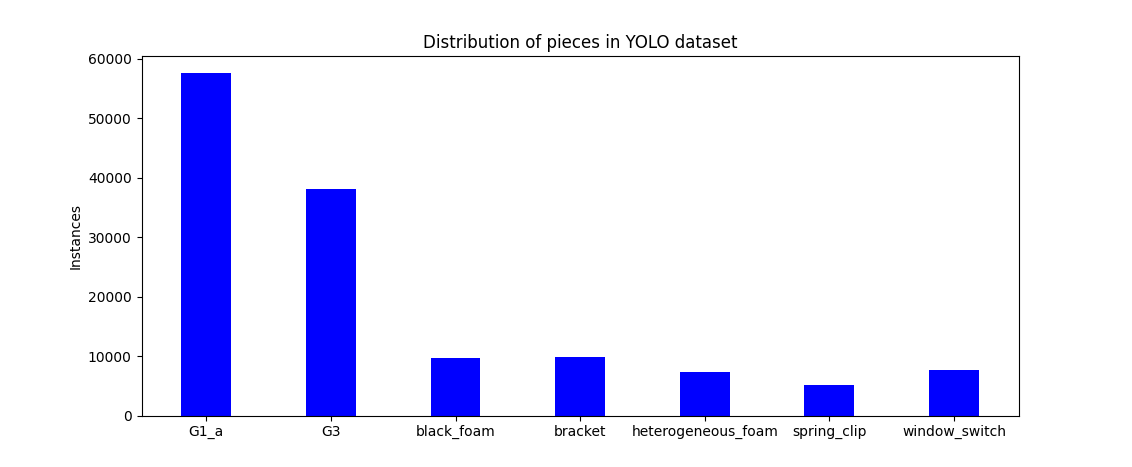
\includegraphics[width=\linewidth]{Dataset/instances_yolo.png}
	\end{subfigure}
	\caption{Instancias de cada pieza empleadas para entrenar el modelo basado en YOLO}
	\label{chap:Generación de un dataset fig:Instancias YOLO}
	
	\begin{subfigure}[b]{0.4\linewidth}
		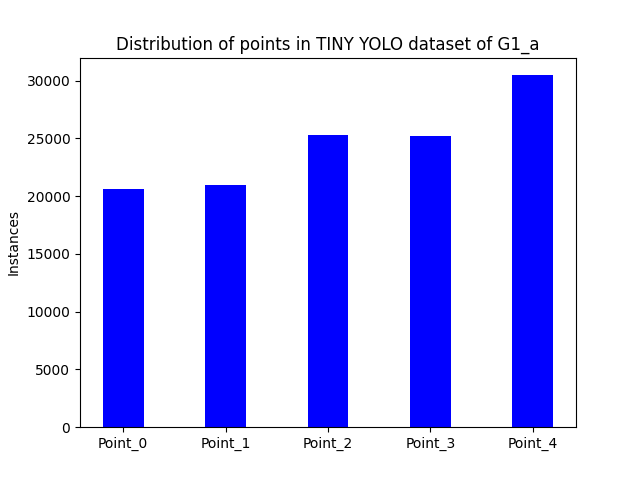
\includegraphics[width=\linewidth]{Dataset/instances_tiny_yolo_G1_a.png}
	\end{subfigure}
	\begin{subfigure}[b]{0.4\linewidth}
		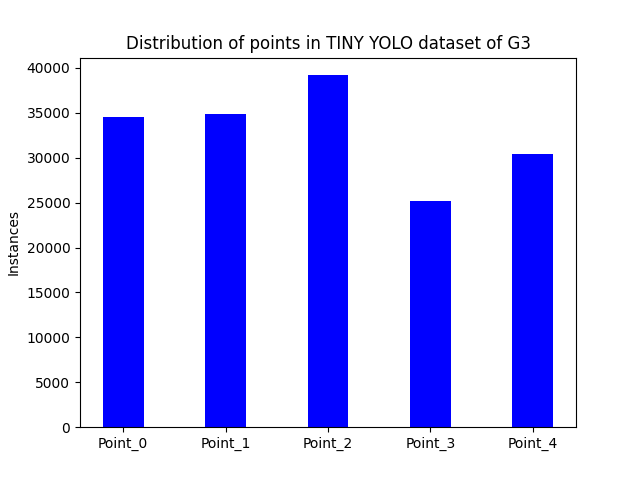
\includegraphics[width=\linewidth]{Dataset/instances_tiny_yolo_G3.png}
	\end{subfigure}
	\caption{Instancias de cada zona de interes empleadas para entrenar el modelo basado en Tiny YOLO}
	\label{chap:Generación de un dataset fig:Instancias Tiny YOLO}
	
	\begin{subfigure}[b]{0.9\linewidth}
		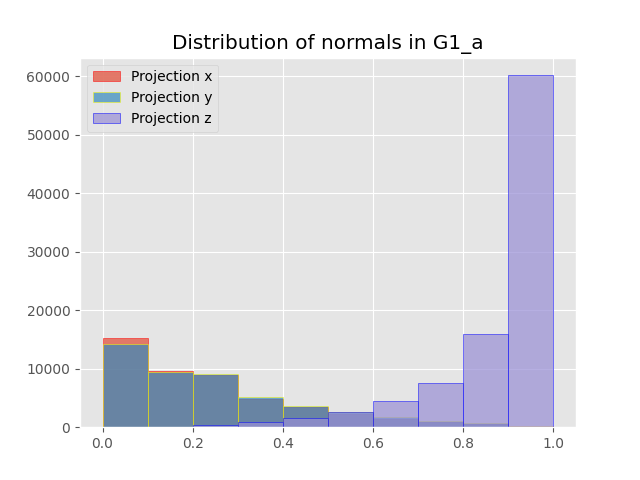
\includegraphics[width=\linewidth]{Dataset/normal_vector_projection_G1_a.png}
	\end{subfigure}
	\caption{Distribución de las proyecciones normales de los puntos de agarre de G1}
	\label{chap:Generación de un dataset fig:Sesgo G1}

\end{figure}


\section{Conclusiones y futuros desarrollos}
Gracias a los resultados mostrados en el capitulo anterior se puede observar el verdadero potencial del generador de imágenes, pero también se aprecia los fallos y puntos de mejora. El sistema ha demostrado ser una opción viable capaz de representar la realidad de forma fiel. Capaz de mantener una constante aleatoriedad a la vez que asegura la replicación. Y ha demostrado ser un sistema adaptable y escalable capaz de trabajar con cualquier tipo de pieza.

Pero a su vez ha mostrado varios fallos de diseño que se deben a error humano y no del sistema. Desgraciadamente el \textit{dataset} generado no es perfecto ya que presenta un elevado sesgo a pesar de representar en gran medida la realidad. A la hora de desarrollar el sistema se enfoco el proyecto en recrear la realidad en lugar de pensar en que tipo de \textit{dataset} se requiere para entrenar la red neuronal. Y debido a la naturaleza de las piezas la realidad es un escenario sesgado en donde la mayoría de las piezas se encuentran en una posición horizontal.

Para evitar este problema en futuros desarrollos se recomienda la introducción de nuevos escenarios con diferentes geometrías que permitan obtener instancias de las piezas con mayor riqueza y en diferentes posiciones. Este tipo de escenarios no deben de presentar un suelo plano sino que deberán de presentar diferentes elevaciones de forma que al apoyarse las piezas no queden en posición horizontal.

  \input{Sistema de visión artificial.tex}
  \chapter{Conclusiones y futuros desarrollos}
\label{chap:Conclusiones y futuros desarrollos}
El desarrollo de este proyecto se caracteriza por cumplir dos grandes objetivos/metas. En primer lugar, su desarrollo ha permitido la creación de un sistema basado en redes neuronales capaz de identificar piezas y sus puntos de agarre óptimos. Y en segundo lugar ha permitido comprobar las capacidades de aprendizaje de una red neuronal al emplear un \textit{dataset} sintético. Es por ello que se debe de analizar el sistema desde las dos perspectivas.

\section{Dataset sintético}
\label{chap:Conclusiones sec:Dataset sintético}
Para el desarrollo del sistema de identificación de puntos de agarre se ha tenido que desarrollar un \textit{dataset} sintético que refleje la realidad y permita aumentar el número de imágenes para el entrenamiento. Este \textit{dataset} se ha realizado con blender y con la ayuda de blenderproc de forma que se ha conseguido generar miles de imágenes fotorealistas que representan y reflejan la zona de trabajo sobre la que se implantará el sistema.

Durante el desarrollo de este sistema se presto especial atención en representar lo mejor posible la realidad y el entorno de trabajo. De esta forma varios de los escenarios y de las configuraciones usadas se limitan a representar los escenarios observados en la planta de ensamblaje. Esta decisión desgraciadamente ha conllevado la generación de un \textit{dataset} sesgado en donde la mayoría de las piezas se encuentran en una posición predefinida por el escenario. Esto ha conllevado a que la red neuronal tienda a asumir que las piezas se encuentran en una de esas posiciones predefinidas y empeore los resultados del sistema.

Es por ello por lo que se recomienda mejorar la aleatoriedad del sistema introduciendo mas escenarios que a pesar de que no reflejen la realidad si permitan la obtención de imágenes con mayor riqueza y eviten el sesgado del la red. Este tipo de escenarios se deben de caracterizar por no presentar un suelo plano sino un suelo con irregularidades que fuercen a las piezas a nuevas posiciones.

\section{Sistema de detección de puntos de agarre}
\label{chap:Conclusiones sec:Sistema de detección de puntos de agarre}
El objetivo final del proyecto es la identificación de puntos de agarre de forma que las piezas puedan ser manipuladas con un robot industrial con el fin de automatizar una linea de ensamblado. La linea de ensamblaje se caracteriza por emplear una elevado diversidad de piezas que presentan diferentes formas y tamaños. Es debido a esta elevada diversidad de piezas que se ha tenido que desarrollar un sistema modular capaz de adaptarse a las diferentes tipos de piezas. El nuevo sistema consta de diferentes módulos/redes que se activan u desactivan en función del tipo de pieza que se desee manipular.

Gracias a este sistema se ha conseguido obtener el punto de agarre óptimo para las piezas grandes y se ha asumido el centro de las piezas pequeñas como un buen punto de agarre. En base a los resultados obtenidos en la fase de validación, el sistema se muestra capaz con errores pequeños y pocos \textit{outliers}. Desgraciadamente el comportamiento de las redes solo se ha podido analizar frente a un \textit{dataset} sintético pero no frente a una situación real. Para determinar con precisión el alcance y la capacidad del sistema se requiere de un \textit{dataset} real.

Pero esta falta de un \textit{dataset} real no impide que se pueda analizar la estructura del sistema y se planteen puntos de mejora. La red presenta grandes puntos fuertes como su modularidad. La cual permite la inclusión de nuevas piezas sin afectar al rendimiento de las ya implementadas y sin la necesidad de entrenar toda la red frente a un \textit{dataset} con todas las piezas. Esto permite reducir los tiempos de entrenamiento de forma sustancial durante el proceso de inclusión de nuevas piezas. Pero a su vez afecta al rendimiento global del sistema ya que implica que se debe de analizar y extraer las características de la pieza varias veces durante su análisis. Por ello se plantea la posibilidad del desarrollo de una única red capaz de aprovechar la extracción de características durante todo el proceso. Este tipo de red aumenta la complejidad del sistema pero permitirá mejorar la eficiencia. Y las últimas capas del sistema deberán de ser intercambiadas dependiendo del tipo de pieza que se vaya a identificar. De esta forma se mantiene la modularidad del sistema pero sin perder la eficiencia propia de estos sistemas.


  \chapter{Objetivos de desarrollo sostenible}
\label{chap:OBS}
\Abstract{Análisis comparativo del proyecto frente a los objetivos de desarrollo sostenible. Desde un punto de visto social, ecológico y económico}
El 25 de septiembre de 2015, los líderes mundiales adoptaron un conjunto de objetivos globales para erradicar la pobreza, proteger el planeta y asegurar la prosperidad para todos como parte de una nueva agenda de desarrollo sostenible. Cada objetivo tiene metas específicas que deben alcanzarse en los próximos 15 años.

\begin{figure}[ht]  %OBS
	\centering
	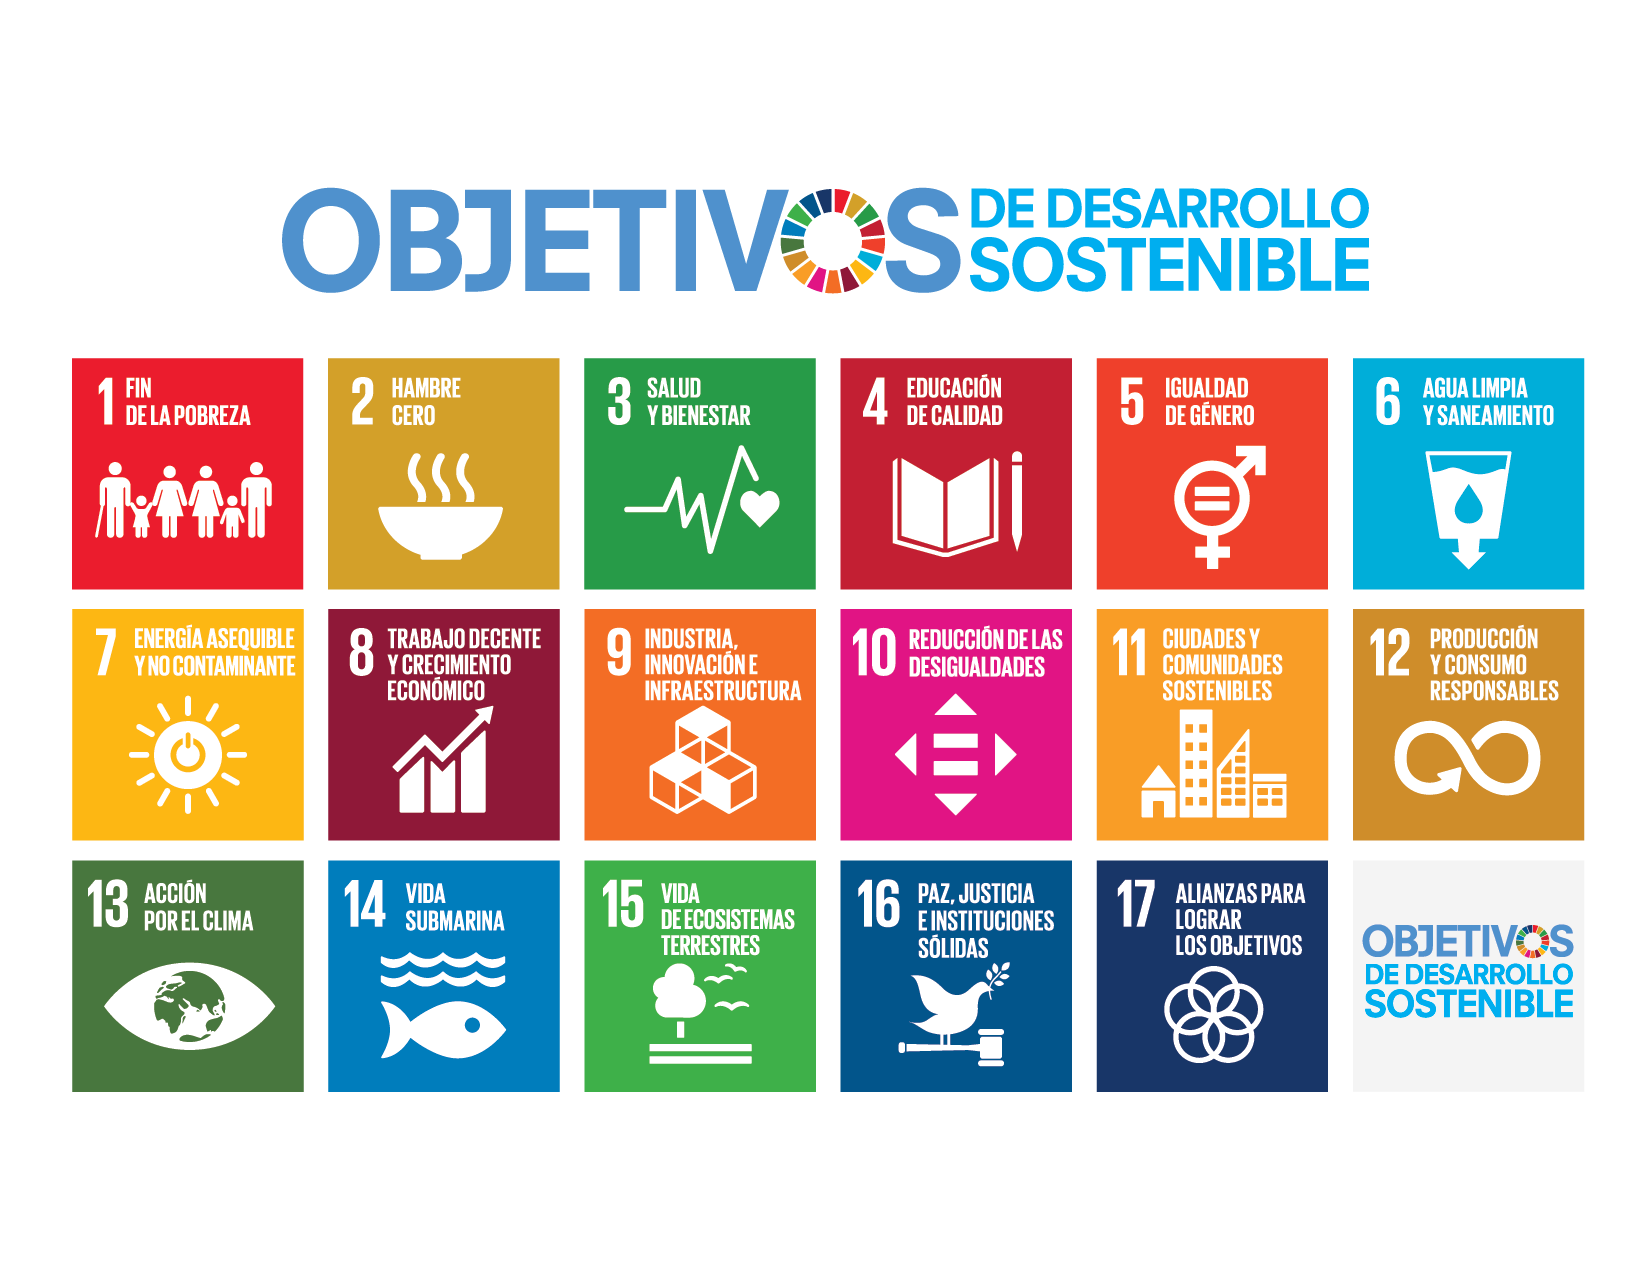
\includegraphics[width=0.8\textwidth]{OBS/esquema.png}
	\vspace{-5pt}
	\caption{Objetivos de desarrollo sostenible aprobados en 2015}
	\label{fig:obs}
\end{figure}

En total se han planteado 17 objetivos para llevar a cabo, este proyecto se enmarca dentro de tres de ellos y a continuación se van a desarrollar de forma individual.

\begin{itemize}
\item Objetivo 8 - Trabajo decente y crecimiento económico: El proceso de automatización de la industria supone la creación de nuevos puestos de trabajo más especializados y con mejores condiciones laborales. Implica un crecimiento de la producción sin un aumento notable de costes y por lo tanto implica un desarrollo económico. Pero par ello es importante controlar este desarrollo y evitar el sobre uso de estas máquinas y con ello el reemplazo del ser humano en el sector industrial.
\item Objetivo 9 - Industria, innovación e infraestructura: Gracias al empleo de las nuevas tecnologías para la automatización de los procesos industriales se ha logrado un crecimiento y desarrollo económico en la industria. Una de las metas de este objetivo es la globalización de estas tecnologías y el facilitar el acceso a estas para los países en vías de desarrollo. Con este proyecto se ha desmostado y creado un sistema reentrenable y usable en el proceso de automatización y esto sin suponer un gran coste de desarrollo. La tecnología desarrollada en este proyecto es de acceso público y modificable para implantar en diferentes sistemas.
\item Objetivo 12 - Producción y consumo responsable: Con la implantación de los robots en la industria no solo se obtiene un incremento en la producción. También, se obtiene una reducción en el número de errores cometidos durante el proceso de fabricación. Esto implica que menos recursos deben de ser usados en la producción. Además, los robots son capaces de desarrollar tareas imposibles para un ser humano y con diferentes materiales. Gracias a sus capacidades, se pueden desarrollar productos más complejos o innovadores centrados en mejorar la sostenibilidad y con un empleo más ecológico de los recursos.
\end{itemize}

Es por todo esto que se considera que este proyecto puede conllevar mejoras para la sociedad a nivel económico, ecológico y social. Siempre y cuando la implantación de estos sistemas se realice correctamente y teniendo en cuenta a la mano de obra humana ya existente. Estos sistemas no deben de reemplazar sino ayudar a este sector.

\appendix  % All chapters below this point will be treated as appendices
  \chapter{Estructura YOLOv5}
\label{apex:Estructura YOLOv5}
Debido al gran interés y las capacidades de YOLO, este ha sido desarrollado bastante en los últimos años. En la actualidad se han publicado cinco versiones de YOLO que mejoran su rendimiento y le dotan de más capacidades. Estas nuevas versiones han traído consigo cambios en la estructura de principal de YOLO para mejorar sus capacidades y rendimiento. A la vez se han desarrollado variantes de la red principal de diferentes tamaños con el fin de poder implantar estos sistemas en sistemas con capacidades computacionales menores. Para el desarrollo de este proyecto nos basaremos en la última versión disponible, la versión cinco que trae consigo un total de diez modelos de diferentes tamaños y resoluciones (ver \autoref{chap:Sistema de visión artificial tab:YOLO models}).

Esta nueva versión trae consigo grandes cambios en la arquitectura empleada la cual se puede dividir en tres secciones:
\begin{itemize}
\item Columna vertebral: Se basa en CSP-Darkent53. Una estructura diseñada con el objetivo de ser empleada para la detección de objetos. Y cuya principal característica es el uso de una estrategia de división y unión que permite mejorar el flujo del gradiente a lo largo de la red.
\item Cuello: Se emplea la nueva función SPPF en lugar de SPP la reduce los tiempos de ejecución a más de la mitad. Se ha desarrollado también un nuevo CSP-PAN.
\item Cabeza: Se vuelve a emplear la cabeza desarrollada en YOLOv3.
\end{itemize}

\begin{figure}[p]
	\centering
	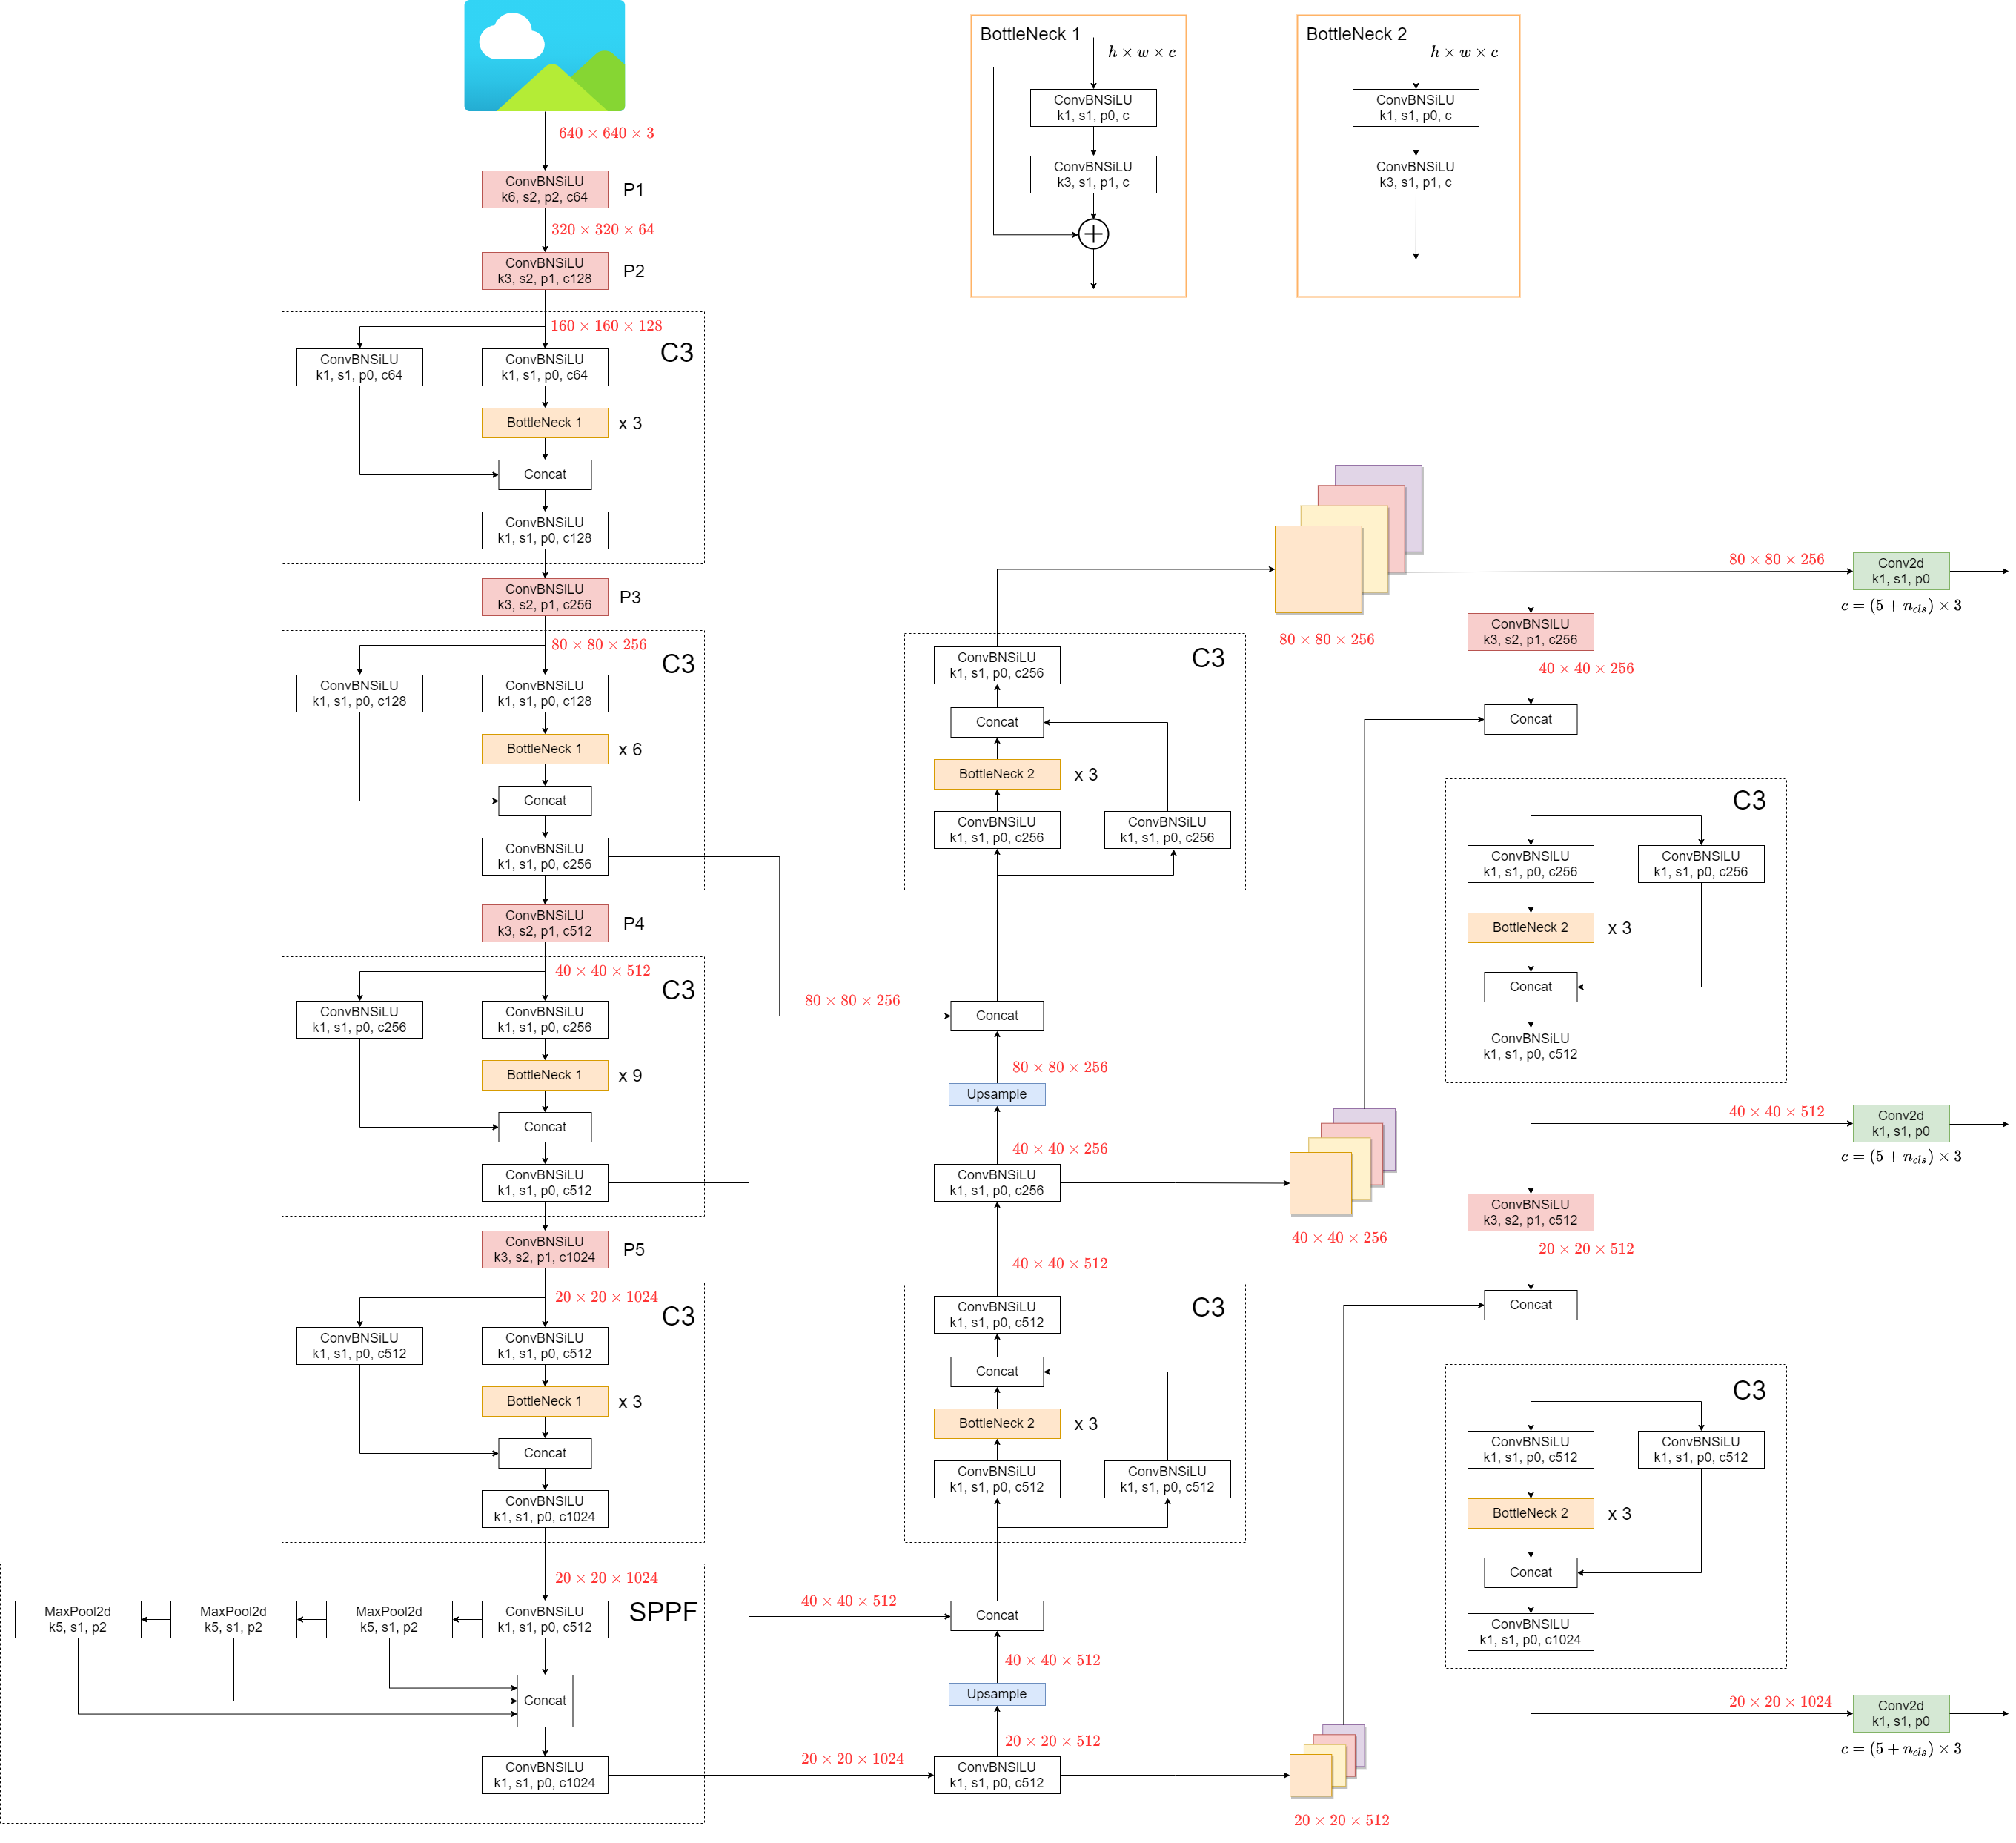
\includegraphics[width=1\textwidth]{Sistema de vision artificial/YOLO/arquitectura.png}
	\caption{Estructura de YOLOv5l}
	\label{chap:Sistema de visión artificial fig:Arquitectura YOLO}
\end{figure}
  \chapter{Camara RGBD}
\label{chap:Camara RGBD}
\Abstract{En este anexo se desarrollará la conexión con la cámara RGBD Intel realsense L515 y las funcionalidades del driver desarrollado.}
Para el desarrollo de este proyecto se ha decidido emplear la cámara Intel Realsense L515 \citep{IntelL515} ya que dispone de todos los sensores necesarios, buenas prestaciones y un reducido coste. Para controlar la cámara se ha desarrollado un \textit{driver} para permitir la conexión directa a través de Python y el \textit{wrapper} desarrollado por Intel.

\begin{figure}[ht]
	\centering
	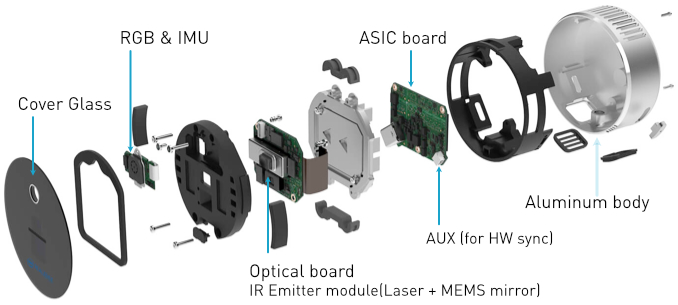
\includegraphics[width=0.95\textwidth]{Camara RGBD/l515_detailed.jpeg}
	\caption[Cámara Intel Realsense L515]{Cámara Intel Realsense L515 \citep{IntelL515}}
	\label{chap:Camara RGBD fig:camara}
\end{figure}

Para la conexión con la cámara se ha desarrollado una clase en Python de forma que el usuario pueda acceder a todas las funciones necesarias de forma cómoda y simple sin necesidad de entender como funciona internamente. La clase se encarga de establecer la conexión con la cámara y al crear nuestra clase en base al \textit{wrapper} desarrollado por Intel, nos permite tener acceso a todas las configuraciones y capacidades de la cámara y basarnos en estas para desarrollar una clase más simple e intuitiva de cara al usuario.

El \textit{driver} se ha desarrollado con varias funcionalidades en mente:
\begin{itemize}
\item Abstracción de la cámara: se desea que durante el desarrollo de las diferentes partes del proyecto no se deba de tener en cuenta la cámara y la configuración de la misma.
\item Independencia del \textit{hardware}: al emplear el mismo \textit{driver} en todas las partes del proyecto, se puede plantear en un futuro un cambio de cámara y el impacto en el proyecto será mínimo.
\item Calibración: el \textit{driver} debe de ser capaz de extraer todo el potencial de la cámara. Esto implica que se debe de añadir la funcionalidad de calibración tanto de las imágenes de color como de profundidad.
\item Alineación: La cámara L515 esta a su vez constituida por diferentes sensores con diferentes parámetros y configuraciones. Con el objetivo de poder relacionar las diferentes imágenes se debe de poder alinear correctamente todas las imágenes.
\end{itemize}

Uno de los puntos más importantes al desarrollar el \textit{driver} ha sido la capacidad de calibración. Al tratarse de diferentes sensores estos deben de estar bien calibrados con sus parámetros intrísecos bien definidos pero a su vez también se deben de definir la relación entre estos sensores con los parámetros extrínsicos. Para la calibración de la cámara de color se pueden emplear varios métodos pero e ha decidido optar por une de los más extendidos basado en la detección de patrones (tablero de ajedrez) con una distancia entre patrones predefinida. Por el contrario, la imagen de profundidad ha sido un mayor obstáculo debido al tipo de tecnología empleada. Al detectar distancias no es capaz de detectar el patrón y por lo tanto en una primera instancia no se puede emplear este método. Este obstáculo se ha conseguido solucionar empleando la imagen de infrarrojos. Esta se obtiene a través del mismo sensor (ambos emplean el sensor \textit{LiDAR}) y es capaz de distinguir el patrón.

\begin{figure}[ht]
  \subfloat{
	\begin{minipage}[c][1\width]{0.3\textwidth}
	   \centering
	   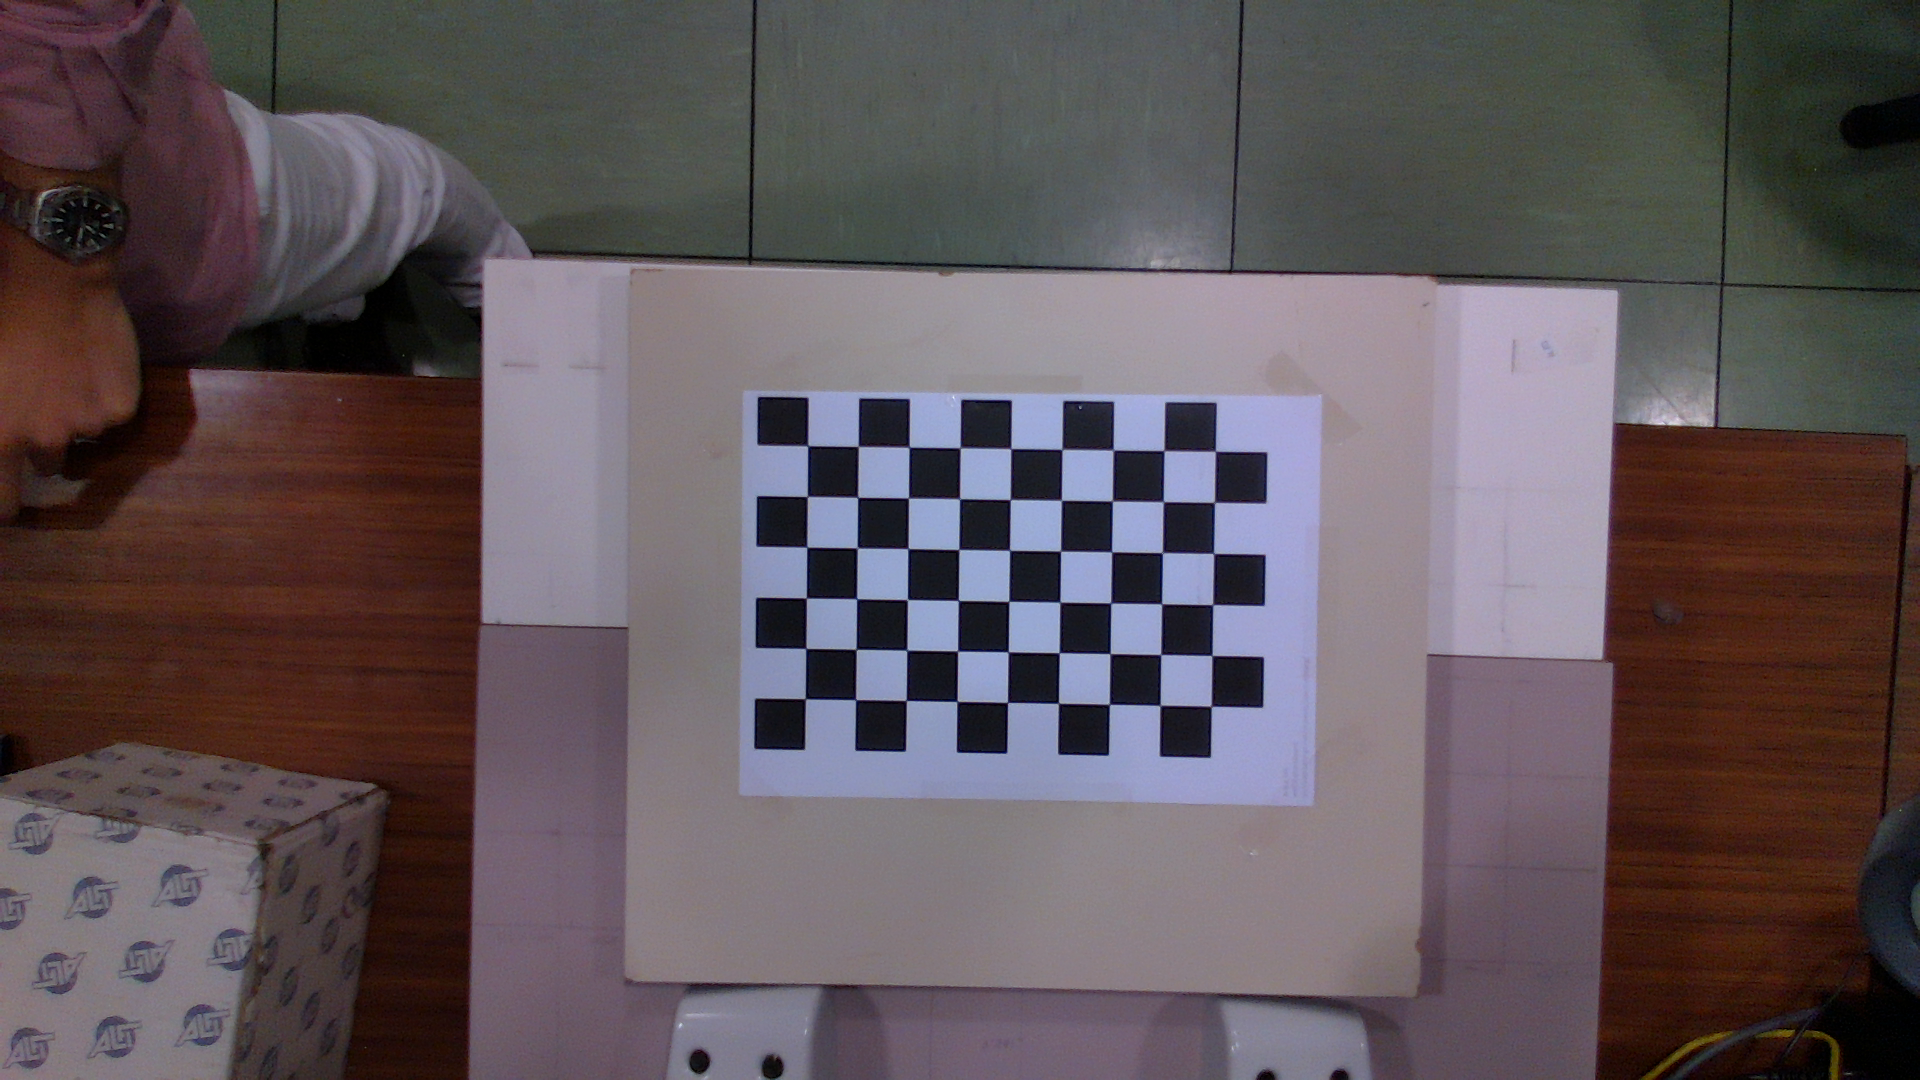
\includegraphics[width=1\textwidth]{Camara RGBD/0000_Colour.png}
	\end{minipage}}
  \hfill	
  \subfloat{
	\begin{minipage}[c][1\width]{0.3\textwidth}
	   \centering
	   \includegraphics[width=1\textwidth]{Camara RGBD/0000_IR.png}
	\end{minipage}}
  \hfill	
  \subfloat{
	\begin{minipage}[c][1\width]{0.3\textwidth}
	   \centering
	   \includegraphics[width=1\textwidth]{Camara RGBD/0000_Depth.png}
	\end{minipage}}
\caption{Comparativa de imágenes de color, infrarrojos y profundidad con Realsense L515}
\label{chap:Camara RGBD fig: Comparativa sensores}
\end{figure}

Tras solucionar los problemas de calibración se ha podido desarrollar el \textit{driver} que tomará el control de la cámara y permitirá abstraer el resto del proyecto del \textit{hardware}. A continuación se muestra la funcionalidad del \textit{driver} desarrollado:

\begin{itemize}
\item Constructor: Se ha desarrollado un constructor personalizado que permite establecer la conexión con la cámara y establecer las opciones de funcionamiento.
\item Destructor: El destructor se ha desarrollado para que durante el proceso de destrucción de la instancia primero se corte de forma gradual la conexión con la cámara. De esta forma se evita futuros errores al intentar reconectarse a la cámara. Si no se realiza una desconexión progresiva no se podrá volver a abrir una conexión con la cámara y será necesario desconectar la cámara o reiniciar el \textit{driver}.
\item setCalibration: Carga y aplica los parámetros definidos por el proceso de calibración.
\item getColour: función para la captura solo de la imagen de color. Devuelve la imagen de color con una resolución de 1920x1080x3 píxeles
\item getDepth: función para la captura solo de la imagen de profundidad. Devuelve la imagen de con o sin alineamiento con la de color y con una resolución de 1024x768 píxeles.
\item getIR: función para la captura solo de la imagen de infrarrojos. Devuelve la imagen de con o sin alineamiento con la de color y con una resolución de 1024x768 píxeles.
\item getImages: Combina las anteriores funciones para obtener la salida de todos los sensores con una sola llamada.
\item saveImages: captura y guarda las imágenes obtenidas por todos los sensores.
\item transformRGBToDepth: relaciona puntos de la imagen de color con la imagen de profundidad (imagen no alineada).
\item getPosition: relaciona un punto en pixeles con sus coordenadas en el mundo real.
\end{itemize}

\begin{figure}[ht]
  \subfloat{
	\begin{minipage}[c][1\width]{0.3\textwidth}
	   \centering
	   \includegraphics[width=1\textwidth]{Camara RGBD/color.png}
	\end{minipage}}
  \hfill	
  \subfloat{
	\begin{minipage}[c][1\width]{0.3\textwidth}
	   \centering
	   \includegraphics[width=1\textwidth]{Camara RGBD/con ajuste.png}
	\end{minipage}}
  \hfill	
  \subfloat{
	\begin{minipage}[c][1\width]{0.3\textwidth}
	   \centering
	   \includegraphics[width=1\textwidth]{Camara RGBD/sin ajuste.png}
	\end{minipage}}
\caption[Alineamiento de imágenes de color y profundidad]{Alineamiento de las imágenes de color y profundidad tomadas con la cámara Realsense L515}
\label{chap:Camara RGBD fig: Alineamiento}
\end{figure}

\backmatter 
  \begingroup
    \setlength\bibitemsep{7pt plus 2pt minus 2pt}
    \phantomsection 
    \addcontentsline{toc}{chapter}{Bibliografía} 
    \printbibliography[title = {Bibliografía}]
  \endgroup  
 
\end{document}